%%%%%%%%%%%%%%%%%%%%%%%%%%%%%%%%%%%%%%%%%%%%%%%%%%%%%%%%%%%%%%%%%%%
%                                                                 %
%   MINUIT - Reference Manual -- LaTeX Source                     %
%                                                                 %
%   Main driver file. Includes the various sources of the manual, %
%   generates the table of contents and includes the index file.  %
%                                                                 %
%   Files referenced: minfront.tex   front material               %
%                     minch1.tex to minch6.tex                    %
%                     minerror.tex                                %
%                     minmain.ind   index made with makeindex     %
%                     cnasbibl.bib   bibliography files (BibTeX)  %
%                                                                 %
%   To run, you need the CERN style cernman.sty                   %
%                                                                 %
%   Editor: Michel Goossens / CN-AS                               %
%   Last Mod.: 20 June 1995 21:00  mg                             %
%                                                                 %
%%%%%%%%%%%%%%%%%%%%%%%%%%%%%%%%%%%%%%%%%%%%%%%%%%%%%%%%%%%%%%%%%%%

\documentclass[11pt]{cernman}
\usepackage{html,alltt,array,color,graphicx,makeidx,verbatim,xspace}
\begin{htmlonly}
\renewcommand{\Cind}[2][]{\texttt{#2}\index{#2@{\ttfamily #2}}}
\renewcommand{\Rind}[2][]{\texttt{#2}\index{#2@{\ttfamily #2}}}
\renewcommand{\Sbox}[4][]{\Sboxni{#3}{#4}% #2 is label
  \label{#2}\index{#3@{\ttfamily #3}|textbf}%
}% ***** end of \newcommand{\Sbox}
\renewcommand{\Sboxni}[3][]{\par% margin note, highlight, parameters
        \begin{tabular}{|lp{15cm}|}\hline
             \quad\textbf{#2}  & \ttfamily #3\\\hline
        \end{tabular}\par
}% ***** end of \newcommand{Sboxni}
\end{htmlonly}
\makeindex
\begin{document}
%  ==================== Front material ============================
%%%%%%%%%%%%%%%%%%%%%%%%%%%%%%%%%%%%%%%%%%%%%%%%%%%%%%%%%%%%%%%%%%%
%                                                                 %
%   MINUIT - Reference Manual -- LaTeX Source                     %
%                                                                 %
%   Front Material: Title page,                                   %
%                   Copyright Notice                              %
%                   Preliminary Remarks                           %
%                   Table of Contents                             %
%   EPS file      : cern15.eps, cnastit.eps                       %
%                                                                 %
%   Editor: Michel Goossens / CN-AS                               %
%   Last Mod.:  18 Aug 1998                                       %
%                                                                 %
%%%%%%%%%%%%%%%%%%%%%%%%%%%%%%%%%%%%%%%%%%%%%%%%%%%%%%%%%%%%%%%%%%%

%%%%%%%%%%%%%%%%%%%%%%%%%%%%%%%%%%%%%%%%%%%%%%%%%%%%%%%%%%%%%%%%%%%%
%    Tile page                                                     %
%%%%%%%%%%%%%%%%%%%%%%%%%%%%%%%%%%%%%%%%%%%%%%%%%%%%%%%%%%%%%%%%%%%%
%begin{latexonly}
\def\Ptitle#1{\special{ps: /Printstring (#1) def}
                       \epsfbox{cnastit.eps}}
\begin{titlepage}
\vspace*{-23mm}
\includegraphics[height=30mm]{cern15.eps}%
\hfill
\raisebox{8mm}{\Large\bf CERN Program Library Long Writeup D506}
\hfill\mbox{}
\begin{center}
\mbox{}\\[10mm]
\mbox{\Ptitle{MINUIT}}\\[1cm]
{\Large Function Minimization and Error Analysis}\\[1cm]
{\LARGE Reference Manual}\\[2cm]
{\LARGE Version 94.1}\\[3cm]
{\Large F. James }\\[1cm]
{\Large Computing and Networks Division}\\[2cm]
\end{center}
\vfill
\begin{center}\Large CERN Geneva, Switzerland\end{center}
\end{titlepage}
%end{latexonly}
\begin{htmlonly}
\begin{center}{\Large\bf CERN Program Library Long Writeup D506}\\[5mm]
{\Huge MINUIT}\\[5mm]
{\Large Function Minimization and Error Analysis}\\[5mm]
{\LARGE Reference Manual}\\[5mm]
{\LARGE Version 94.1}\\[5mm]
{\Large F. James }\\[5mm]
{\Large Computing and Networks Division}\\[5mm]
{\Large CERN Geneva, Switzerland}\\[5mm]
\end{center}

\begin{rawhtml}
<HR>
<H3><A href="http://wwwinfo.cern.ch/asd/cernlib/minuit/minuit.ps">
PostScript version of this manual</A></H3>
<HR>
\end{rawhtml}
\end{htmlonly}



%%%%%%%%%%%%%%%%%%%%%%%%%%%%%%%%%%%%%%%%%%%%%%%%%%%%%%%%%%%%%%%%%%%%
%    Copyright  page                                               %
%%%%%%%%%%%%%%%%%%%%%%%%%%%%%%%%%%%%%%%%%%%%%%%%%%%%%%%%%%%%%%%%%%%%
\begin{htmlonly}
\chapter{Copyright Notice}
\end{htmlonly}
%begin{latexonly}
\thispagestyle{empty}
\framebox[\textwidth][t]{\hfill\begin{minipage}{0.96\textwidth}%
\vspace*{3mm}
\begin{center}Copyright Notice\end{center}
\parskip\baselineskip
%end{latexonly}
{\bf MINUIT -- Function Minimization and Error Analysis}
\par 
CERN Program Library entry {\bf D506}
\par
\copyright{} Copyright CERN, Geneva 1994--1998
\par
Copyright and any other appropriate legal protection of these
computer programs and associated documentation reserved in all
countries of the world.
\par
These programs or documentation may not be reproduced by any
method without prior written consent of the Director-General
of CERN or his delegate.
\par
Permission for the usage of any programs described herein is
granted apriori to those scientific institutes associated with
the CERN experimental program or with whom CERN has concluded
a scientific collaboration agreement.
\par
Requests for information should be addressed to:
%begin{latexonly}
\vspace*{-.5\baselineskip}
\begin{center}
\tt\begin{tabular}{l}
CERN Program Library Office              \\
CERN-IT Division                         \\
CH-1211 Geneva 23                        \\
Switzerland                              \\
Tel.      +41 22 767 4951                \\
Fax.      +41 22 767 8630                \\
Internet: cernlib@cern.ch                
\end{tabular}
\end{center}
\vspace*{2mm}
\end{minipage}\hfill}%end of minipage in framebox
\vspace{6mm}
%end{latexonly}
\begin{htmlonly}
\par
\begin{flushleft}
CERN Program Library Office              \\
CERN-IT Division                         \\
CH-1211 Geneva 23                        \\
Switzerland                              \\
Tel.: +41 22 767 4951                    \\
Fax.: +41 22 767 8630                    \\
Internet: \texttt{cernlib@cern.ch}                
\end{flushleft}
\par
\end{htmlonly}

%begin{latexonly}
{\bf Trademark notice: All trademarks appearing in this guide are acknowledged as such.}
\vfill
\begin{tabular}{l@{\quad}l@{\quad}>{\tt}l}
\emph{Contact Person}:           & Ian McLaren     /IT &(Ian.Mclaren\atsign cern.ch)\\[1mm]
\emph{Cocumentation consultant}: & Michel Goossens /CN &(goossens\atsign cern.ch)\\[1cm]
{\em Edition -- August 1998}
\end{tabular}
%end{latexonly}
\begin{htmlonly}
{\bf Trademark notice: All trademarks appearing in this guide are acknowledged as such.}

\begin{tabular}{lll}
\emph{Contact Person}:           & Ian McLaren /IT     & \texttt{Ian.Mclaren@cern.ch}\\
\emph{Documentation consultant}: & Michel Goossens /IT & \texttt{goossens@cern.ch}\\
\emph{Edition -- August 1998}
\end{tabular}
\end{htmlonly}
\newpage
 
%%%%%%%%%%%%%%%%%%%%%%%%%%%%%%%%%%%%%%%%%%%%%%%%%%%%%%%%%%%%%%%%%%%%
%    Introductory material                                         %
%%%%%%%%%%%%%%%%%%%%%%%%%%%%%%%%%%%%%%%%%%%%%%%%%%%%%%%%%%%%%%%%%%%%
%begin{latexonly}
\pagenumbering{roman}
\setcounter{page}{1}

\chapter*{Foreword}

\section*{What Minuit is intended to do.}
%end{latexonly}
\begin{htmlonly}
\chapter{Foreword}
\subsection*{What Minuit is intended to do.}
\end{htmlonly}
Minuit is conceived as a tool to find the minimum value of a
multi-parameter function and analyze the shape of the function around
the minimum. The principal application is foreseen for statistical
analysis, working on chisquare or log-likelihood functions, to compute
the best-fit parameter values and uncertainties, including
correlations between the parameters.  It is especially suited to
handle difficult problems, including those which may require guidance
in order to find the correct solution.
%begin{latexonly}
\section*{What Minuit is not intended to do.}
%end{latexonly}
\begin{htmlonly}
\subsection*{What Minuit is not intended to do.}
\end{htmlonly}

Although Minuit will of course solve easy problems faster than complicated
ones, it is not intended for the repeated solution of identically parametrized
problems (such as track fitting in a detector) where a specialized
program will in general be much more efficient.
 
%begin{latexonly}

\section*{Further remarks.}
 
In this manual examples are in {\tt monotype face} and strings to be
input by the user are {\tt\underline{underlined}}.  In the index the
page where a routine is defined is in {\bf bold}, page numbers where a
routine is referenced are in normal type.  In the description of the
routines a \texttt{*} following the name of a parameter indicates that
this is an {\bf output} parameter.  If another \texttt{*} precedes a
parameter in the calling sequence, the parameter in question is both
an {\bf input} and {\bf output} parameter.

This document has been produced using \LaTeX~\cite{bib-LATEX} with the
\texttt{cernman} style option, developed at CERN.  A compressed
PostScript file \texttt{minuit.ps.gz}, containing a complete printable
version of this manual, can be obtained from any CERN machine by
anonymous ftp as follows (commands to be typed by the user are
underlined):

\vspace*{3mm} 
\begin{alltt}\footnotesize
    \underline{ftp asis01.cern.ch}
    Trying 128.141.201.136...
    Connected to asis01.cern.ch.
    220 asis01 FTP server (Version 6.10 ...) ready.
    Name (asis01:username): \underline{anonymous}
    Password: \underline{your\_{}mailaddress}
    230 Guest login ok, access restrictions apply.
    ftp> \underline{cd cernlib/doc/ps.dir}
    ftp> \underline{get minuit.ps}
    ftp> \underline{quit}
\end{alltt}

%%%%%%%%%%%%%%%%%%%%%%%%%%%%%%%%%%%%%%%%%%%%%%%%%%%%%%%%%%%%%%%%%%%%
%    Tables of contents ...                                        %
%%%%%%%%%%%%%%%%%%%%%%%%%%%%%%%%%%%%%%%%%%%%%%%%%%%%%%%%%%%%%%%%%%%%

\newpage
\tableofcontents
%\newpage
\listoffigures
\listoftables
%end{latexonly}

%  ==================== Body of text ==============================
\pagenumbering{arabic}
\setcounter{page}{1}
%%\part{Minuit User's Guide}
%%%%%%%%%%%%%%%%%%%%%%%%%%%%%%%%%%%%%%%%%%%%%%%%%%%%%%%%%%%%%%%%%%%
%                                                                 %
%   MINUIT User Guide -- LaTeX Source                             %
%                                                                 %
%   Chapter 1                                                     %
%                                                                 %
%   The following external EPS files are referenced:              %
%                                                                 %
%   Editor: Michel Goossens / CN-AS                               %
%   Last Mod.: 17 Mar. 1992 10:00 mg                              %
%                                                                 %
%%%%%%%%%%%%%%%%%%%%%%%%%%%%%%%%%%%%%%%%%%%%%%%%%%%%%%%%%%%%%%%%%%%
 
\chapter{Minuit Basic Concepts}

\section{The Organization of Minuit.}
The Minuit package acts on a multiparameter Fortran function to which we
give the generic name \Rind{FCN}, although the actual name may be chosen by the user.
This function must be defined and supplied by the user (or by an intermediate
program such as HBOOK\cite{bib-HBOOK} or PAW\cite{bib-PAW}, 
in case Minuit is being used under the
control of such an intermediate program).
The value of \Rind{FCN} will in general depend on one or more variable parameters
whose meaning is defined by the user (or by the intermediate program),
but whose trial values are determined by Minuit according to what the user
requests should be done to \Rind{FCN} (usually minimize it).
 
To take a simple example, suppose the problem is to fit a polynomial through
a set of data points.
Then the user would write an \Rind{FCN} which calculates the chisquare between a
polynomial and the data; the variable parameters of \Rind{FCN} would be the
coefficients of the polynomials.  Using Minuit commands, the user would request
Minuit to minimize \Rind{FCN} with respect to the parameters, that is, find those
values of the coefficients which give the lowest value of chisquare.
 
The user must therefore supply, in addition to the function to be analyzed,
a set of commands to instruct Minuit what analysis is wanted.
The commands may be given in several different forms:

\begin{UL}
\item As a data file, corresponding to the traditional ``data cards'', for
      batch processing;
\item Typed in at execution time at a terminal, for interactive running;
\item Coded in Fortran in the calling program, which allows looping,
      conditional execution, and all the other possibilities of Fortran, but not
      interactivity, since it must be compiled before execution.
      This is sometimes known as running Minuit in ``slave mode''.
      HBOOK and PAW use Minuit in this way.
\end{UL}

It is also possible to mix any of the above forms, for example starting off
a fit with a standard command file, then turning it over to the interactive
user for the final command steps.

\section{Internal and External Parameters.}

\index{internal parameter}
\index{external parameter}
\index{parameters!external}
\index{parameters!internal}
Each of the parameters to \Rind{FCN} is defined by the user as belonging to
one of the following types:

\begin{DL}{Variable with limits:\ }
\item[Freely variable:]      allowed to take on any value.
\item[Variable with limits:] allowed to vary only between two limits specified by the user.
\item[Fixed:]                originally defined as variable, but now taking on only the
                             value the parameter had at the moment it was fixed, 
                             or a value later assigned by the user.
\item[Constant:]             taking on only one value as specified by the user.
\item[Undefined:]            never defined by user.
\end{DL}
 
The user, in \Rind{FCN}, must of course be able to ``see'' all types of
defined parameters,
and he therefore has access to what we call the
{\it external parameter list}, that is, the parameters as he
defined them.
On the other hand, the internal Minuit minimizing routines only want to ``see''
variable parameters without limits, and so they have access only to the
{\it internal parameter list} which is created from the external list
by the following transformation:

\begin{OL}
\item Squeeze out all parameters that are not variable.
\item Transform all variable parameters with limits, so that the transformed
      parameter can vary without limits.
      (See the next section for details concerning this transformation.)
      Because this transformation is non-linear, it is recommended to avoid
      putting limits on parameters where they are not needed.
\end{OL}

As an example, suppose that the user has defined the following parameters:
\begin{UL}
\item Parameter 1, constant.
\item Parameter 3, freely variable.
\item Parameter 10, variable with limits.
\item Parameter 11, constant.
\item Parameter 22, freely variable.
\item All others undefined.
\end{UL}
Then the internal parameter list would be as follows:
\begin{UL}
\item Internal parameter 1 = external parameter 3.
\item Internal parameter 2 = external parameter 10, transformed appropriately.
\item Internal parameter 3 = external parameter 22.
\end{UL}
\index{internal parameter}
\index{external parameter}
\index{parameters!external}
\index{parameters!internal}
In the above example, Minuit considers that the number of external parameters
is 22 (the highest external parameter number defined), and the number of
internal parameters is 3.  The latter number is passed as \texttt{NPAR} to \Rind{FCN}.
This is the number which determines, for example, the size of the error matrix
of the parameters, since only variable parameters have errors.
 
An important feature of Minuit is that parameters are allowed to change
types during a Minuit run. Several Minuit commands are available to make
variable parameters fixed and vice-versa; to impose, change, or remove limits
from variable parameters; and even to define completely new parameters at any
time during a run. In addition, some Minuit routines (notably the \Cind[MINOs]{MINOS} error
analysis) cause one or more variable parameters to be temporarily fixed during
the calculation.  Therefore, the correspondence between external and internal
parameter lists is in general a dynamic one, and the value of \texttt{NPAR} is not
necessarily constant.

\subsection{The transformation for parameters with limits.}

For variable parameters with limits, Minuit uses the following transformation:
$$
\begin{array}{l@{\hspace{3cm}}l}
P_{\mathrm{int}} = \arcsin
        \left( 2\: \frac{\Tstm P_{\mathrm{ext}}-a\Rule}{\Tstm b-a} - 1 \right)       &
P_{\mathrm{ext}} = a + \frac{\Tstm b - a}{\Tstm 2}
        \left( \sin P_{\mathrm{int}} + 1 \right)                  \\
\end{array}
$$
so that the internal value $P_{\mathrm{int}}$ can take on any value, while
the external value $P_{\mathrm{ext}}$ can take on values only between the lower
limit $a$ and the upper limit $b$.
Since the transformation is necessarily non-linear, it would transform a
nice linear problem into a nasty non-linear one, which is the reason why
limits should be avoided if not necessary. 
In addition, the transformation
does require some computer time, so it slows down the computation a little
bit, and more importantly, it introduces additional numerical inaccuracy into
the problem in addition to what is introduced in the numerical calculation
of the \texttt{FCN} value.  
The effects of non-linearity and numerical roundoff both
become more important as the external value gets closer to one of the limits
(expressed as the distance to nearest limit divided by distance between limits).
The user must therefore be aware of the fact that, for example,
if he puts limits of $(0,10^{10})$ on a parameter, then the values $0.0$ 
and $1.0$ will be indistinguishable to the accuracy of most machines.

The transformation also affects the parameter error matrix, of course,
so Minuit does a transformation of the error matrix (and the 
``parabolic'' parameter errors) when there are parameter limits.
Users should however realize that the transformation is only a linear
approximation, and that it cannot give a meaningful result if one or more
parameters is very close to a limit, where
$\partial P_{\mathrm{ext}} / \partial P_{\mathrm{int}} \approx 0$.
Therefore, it is recommended that:
\begin{UL}
\item Limits on variable parameters should be used only when needed in order
to prevent the parameter from taking on unphysical values.
\item When a satisfactory minimum has been found using limits, the limits
should then be removed if possible, in order to perform or re-perform the
error analysis without limits.
\end{UL}

Further discussion of the effects of parameter limits may be
found in the last chapter.

\section{Minuit Strategy.}

At many places in the analysis of the user function, Minuit must
decide whether to be ``safe'' and waste a few function calls in order
to know where it is, or to be ``fast'' and attempt to get the requested
results with the fewest possible calls at a certain risk of not
obtaining the precision desired by the user.
In order to allow the user to influence these decisions, there is an
internal Minuit parameter \texttt{ISTRAT} which can be set by the user
through the command \Cind{SET STRategy}.  
In the current release,
this parameter can take on three integer values (0, 1, 2), and the
default value is 1.  Value 0 indicates to Minuit that it should
economize function calls; it is intended for cases where there are
many variable parameters and/or the function takes a long time
to calculate and/or the user is not interested in very precise
values for parameter errors.  On the other hand, the value 2 indicates
that Minuit is allowed to waste function calls in order to be sure
that all values are precise; it is intended for cases where the function
is evaluated in a very short time and/or where the parameter errors
must be calculated reliably

\section{Parameter Errors.}

Minuit is usually used to find the ``best'' values of a set of parameters,
where ``best'' is defined as those values which minimize a given function, \Rind{FCN}.
The width of the function minimum, or more generally, the shape of the
function in some neighbourhood of the minimum, gives information about
the {\it uncertainty} in the best parameter values, often called by
physicists the {\it parameter errors}.
An important feature of Minuit is that it offers several tools to analyze
the parameter errors.
\subsection{FCN Normalization and the ERRor definition.}
Whatever method is used to calculate the parameter errors, they will depend
on the overall (multiplicative) normalization of \Rind{FCN}, in the sense that if
the value of \Rind{FCN} is everywhere multiplied by a constant $\beta$, then the errors
will be decreased by a factor $\sqrt{\beta}$.
Additive constants do not change the parameter
errors, but may imply a different goodness-of-fit confidence level.
 
Assuming that the user knows what the normalization of his \Rind{FCN} means, and
also that he is interested in parameter errors, the \Cind{SET ERRordef} command
allows him to define what he means by one ``error'', in terms of the
change in \Rind{FCN} value which should be caused by changing one parameter by
one ``error''.  
If the \Rind{FCN} is the usual chisquare function (defined below),
then \Cind[SET ERRordef]{ERRordef} should be set to 1.0 
(the default value anyway) if the user
wants the usual one-standard-deviation errors.
If \Rind{FCN} is a negative-log-likelihood
function, then the one-standard-deviation value for 
\Cind[SET ERRordef]{ERRORDEF} is 0.5.
If \Rind{FCN} is a chisquare, but the user wants two-standard-deviation errors, then
\Cind[SET ERRordef]{ERRORDEF} should be = 4.0, etc.
 
Note that in the usual case where Minuit is being used to perform a fit to
some experimental data, the parameter errors will be proportional to the
uncertainty in the data, and therefore meaningful parameter errors cannot
be obtained unless the measurement errors of the data are known.  In the common
case of a least-squares fit, \Rind{FCN} is usually defined as a chisquare:

\begin{equation}
\chi^2 (\alpha) = \sum_{i=1}^{n} \frac{f(x_i,\alpha) - e_i)^2}{\sigma_i^2}
\end{equation}

where $\alpha$ is the vector of free parameters being fitted, and
the $\sigma_i$ are the uncertainties in the individual measurements $e_i$.
If these uncertainties are not known, and are simply left out of the calculation,
then the fit may still have meaning, but not the quantitative values of the
resulting parameter errors.
(Only the relative errors of different parameters with
respect to each other may be meaningful.)
 
If the $\sigma_i$ are all overestimated by a factor $\beta$, then the resulting
parameter errors from the fit will be overestimated by the same factor $\beta$.

\subsection{The Error Matrix.}

The Minuit processors \Cind[MIGrad]{MIGRAD} and \Cind[HESse]{HESSE} 
normally produce an error matrix.
This matrix is the inverse of the matrix of second derivatives of \Rind{FCN},
transformed if necessary into external coordinate space%
\footnote{The {\it internal error matrix} maintained by Minuit is transformed
for the user into {\it external coordinates}, but the numbering
of rows and columns is of course still according to internal parameter
numbering, since one does not want rows and columns corresponding to
parameters which are not variable. The transformation therefore
affects only parameters with limits; if there are no limits, internal and
external error matrices are the same.},
and multiplied by the square root of \Cind[SET ERRordef]{ERRORDEF}.
Therefore, errors based on the Minuit error matrix take account of all the
parameter correlations, but not the non-linearities. That is, from the error
matrix alone, two-standard-deviation errors are always exactly twice as big
as one-standard-deviation errors.
 
When the error matrix has been calculated (for example by the successful
execution of a command \Cind{MIGrad} or \Cind{HESse}) then the parameter errors
printed by Minuit are the square roots of the diagonal elements of this
matrix. The commands \Cind{SHOw COVariance} and \Cind{SHOw CORrelations}
allow the user to see the off-diagonal elements as well.
The command \Cind{SHOw EIGenvalues} causes Minuit to calculate and print
out the eigenvalues of the error matrix, which should all be
positive if the matrix is positive-definite (see below on Migrad and
positive-definiteness).
 
The effect of correlations on the individual parameter errors can be
seen as follows. When parameter \texttt{N} is \Cind{FIX}ed, 
Minuit inverts the error
matrix, removes the row and column corresponding to parameter \texttt{N}, and
re-inverts the result. The effect on the errors of the other parameters
will in general be to make them smaller, since the component due to
the uncertainty in parameter \texttt{N} has now been removed. (In the limit
that a given parameter is uncorrelated with parameter \texttt{N}, its error will
not change when parameter \texttt{N} is fixed.)
However the procedure is not reversible, since Minuit forgets the
original error matrix, so if parameter \texttt{N} is then \Cind{RELease}d, 
the error matrix is considered as unknown and has to be recalculated with
appropriate commands.

\subsection{MINOS Errors.}
\index{errors}

The Minuit processor \Cind[MINOs]{MINOS} was probably the first, and may still be the only,
generally available program to calculate parameter errors taking into
account both parameter correlations and non-linearities.
The \Cind[MINOs]{MINOS} error intervals are in general assymmetric, and may be expensive
to calculate, especially if there are a lot of free parameters and the
problem is very non-linear.
 
\Cind[MINOs]{MINOS} can only operate after a good minimum has already been found, and
the error matrix has been calculated, so the \Cind[MINOs]{MINOS} command will
normally follow a \Cind[MIGrad]{MIGRAD} command.
The \Cind[MINOs]{MINOS} error for a given parameter is defined as the change in the
value of that parameter which causes $F'$ to increase by the amount \texttt{UP},
where $F'$ is the minimum of \Rind{FCN} with respect to all {\it other}
free parameters, and \texttt{UP} is the ERRordef value specified by the
user (default = 1.).
 
The algorithm for finding the positive and negative \Cind[MINOs]{MINOS} errors for
parameter \texttt{N} consists of varying parameter \texttt{N}, each time minimizing
\Rind{FCN} with respect to all the other \texttt{NPAR-1} variable parameters,
to find numerically the two values of parameter \texttt{N} for which the
minimum of \Rind{FCN} takes on the values \texttt{FMIN+UP}, where \texttt{FMIN} is the
minimum of \Rind{FCN} with respect to all \texttt{NPAR} parameters.
In order to make the procedure as fast as possible, \Cind[MINOs]{MINOS} uses the
error matrix to predict the values of all parameters at the
various sub-minima which it will have to find in the course of the
calculation, and in the limit that the problem is nearly linear,
the predictions of \Cind[MINOs]{MINOS} will be nearly exact, requiring very
few iterations.  On the other hand, when the problem is very
non-linear (i.e., \Rind{FCN} is far from a quadratic function of its
parameters), that is precisely the situation when \Cind[MINOs]{MINOS} is needed
in order to indicate the correct parameter errors.

\subsection{Contour Plotting}

Minuit currently offers two very different procedures for finding
\Rind{FCN} contours.  They will be identified by the corresponding
command names: \Cind{CONtour} and \Cind{MNContour}.
 
\subsubsection{CONtour}

This procedure is designed for a lineprinter or alphanumeric
terminal as output device, and gives a static picture of \Rind{FCN}
as function of the two parameters specified by the user, that is,
all the other variable parameters (if any) are considered as
temporarily fixed at their current values.  First a range is
chosen, by default two current standard deviations on either
side of the current best value of each of the two parameters,
and a grid size n is chosen, by default 25 by 25 positions
for the full range of each parameter.  Contour zero is defined
as the current best function value $\displaystyle F_{\mathrm{min}}$
(presumably the minimum), and then the $\displaystyle i^{\mathrm{th}}$
contour is defined as where \Rind{FCN} has the value
$\displaystyle F_{\mathrm{min}} + i^2 * \mbox{\tt UP}$.
The procedure then simply evaluates \Rind{FCN} at the four corners of
each of the $n^2$ grid positions (which makes $(n+1)^2$ evaluations)
to determine whether the $\displaystyle i^{\mathrm{th}}$ contour passes through
it. The method, although not very efficient or precise,
is very robust, and capable of revealing unexpected
multiple valleys.
 
\subsubsection{MNContour}

The contour calculated by \Cind{MNContour} is dynamic, in the sense
that it represents the minimum of \Rind{FCN} with respect to all the
other \texttt{NPAR-2} parameters (if any). In statistical terms, this
means that \Cind{MNContour} takes account of the correlations between
the two parameters being plotted, and all the other variable
parameters, using a procedure analogous to that of \Cind[MINOs]{MINOS}.
(If this feature is not wanted, then the other
parameters must be \Cind{FIX}ed before calling \Cind{MNContour}.)
\Cind{MNContour} provides the actual coordinates of the points around
the contour, suitable for plotting with a graphics routine or
by hand. The points are given in counter-clockwise order
around the contour.
Only one contour is calculated per command (or Fortran call),
and the level is $\displaystyle F_{\mathrm{min}} + \mbox{\tt UP}$.
where \texttt{UP} is the
\Cind[SET ERRordef]{ERRordef} specified by the user, or 1.0 by default.
The number of points to be calculated is chosen by
the user (Default is 20 for the data-driven mode.).
As a by-product, \Cind{MNContour} provides the \Cind[MINOs]{MINOS} errors of the
two parameters in question, since these are just the extreme
points of the contour (Use \Cind{SHOw MINos} to see them).
In command-driven mode, a rough (alphanumeric, not graphic)
plot of the points is given 
(if \Cind[SET PRIntout]{PRIntlevel$\geq0$}) 
and the numerical values of the coordinates are printed 
(if \Cind[SET PRIntout]{PRIntlevel$\geq1$}).
In Fortran-callable mode, the user gets Fortran
access to the vector of point coordinates through
\Rind[MNCONT]{SUBROUTINE MNCONT}.

%%%%%%%%%%%%%%%%%%%%%%%%%%%%%%%%%%%%%%%%%%%%%%%%%%%%%%%%%%%%%%%%%%%
%                                                                 %
%   MINUIT User Guide -- LaTeX Source                             %
%                                                                 %
%   Chapter 2                                                     %
%                                                                 %
%   The following external EPS files are referenced:              %
%                                                                 %
%   Editor: Michel Goossens / CN-AS                               %
%   Last Mod.:  1 Apr. 1992 10:10 mg                              %
%                                                                 %
%%%%%%%%%%%%%%%%%%%%%%%%%%%%%%%%%%%%%%%%%%%%%%%%%%%%%%%%%%%%%%%%%%%
 
\chapter{Minuit Installation.}

\section{Minuit Releases.}
 
Minuit has been extensively revised in 1989, but the usage is
largely compatible
with that of older versions which have been in use since before 1970.
Users familiar with older releases, who have not yet used releases
from 1989 or later, must however read this manual, in order to
adapt to the few changes as well as to discover the new features
and easier ways of using old features, such as free-field input.

\section{Minuit Versions.}

The program is entirely in standard portable Fortran 77,
and requires no external subroutines except those defined as part of
the Fortran 77 standard and one logical function \Rind{INTRAC}
\footnote{\Rind{INTRAC} is available from the CERN Program Library 
for all common
computers, and in the worst case can be replaced by a \Lit{LOGICAL FUNCTION}
returning a value of \Lit{.TRUE.} or \Lit{.FALSE.} depending on
whether or not Minuit is being used interactively.}.
The only difference between versions for different computers,
apart from \Rind{INTRAC}, is the floating point precision (see heading below).
 
As with previous releases, Minuit does not use a memory manager.
This makes it easy to install and independent of other programs,
but has the disadvantage that both the memory occupation and the
maximum problem size (number of parameters) are fixed at compilation
time.
The old solution to this problem, which consisted of providing
``long'' and ``short'' versions, has proved to be somewhat clumsy and
anyway insufficient for really exceptional users, so it has been
abandoned in favour of a single ``standard'' version.
 
\index{parameters!number of}
\index{version}
\index{variable}
The currently``standard'' version of Minuit
will handle functions of up to 100
parameters, of which not more than 50 can be variable at one time.
Because of the use of the \Lit{PARAMETER} statement in the Fortran source,
redimensioning for larger (or smaller) versions is very easy
(although it will help to have a source code manager or a good editor
to propagate the modified \Lit{PARAMETER} statement through all the
subroutines, and of course it implies recompilation).
The definition of what is ``standard'' may well change in the light of
experience (it was 35 instead of 50 variable parameters for
release 89.05),
and it is likely that different installations will wish
to define it differently according to their own applications.
In any case, the dimensions used at compilation time are printed
in the program header at execution time, and the program is of course
protected against the user trying to define too many parameters.
The user who finds that the version available to him is too small
(or too big) must try to convince his computer manager to change the
installation default or to provide an additional special version,
or else he must obtain the source and recompile his own version.
\section{Interference with Other Packages}
The new Minuit has been designed to interfere as little as possible
with other programs or packages which may be loaded at the same
time. Thus it uses no memory manager or other external subroutines
(except \Lit{LOGICAL FUNCTION INTRAC}), all its own subroutine names
start with the letters \Lit{MN}
(except Minuit and the user written routines),
all \Lit{COMMON} block names start with the characters \Lit{MN7},
and the user should not need to use explicitly any
Minuit \Lit{COMMON} blocks.
 
In addition, more than one different functions can be minimized in the
same execution module, provided the functions have different names,
and provided one minimization and error analysis is completely
finished before the next one begins.

\section{Floating-point Precision}

It is recommended for most applications to use 64-bit floating point
precision, or the nearest equivalent on any particular machine.
This means that the standard Minuit installed on Vax, IBM
and Unix workstations will normally be the \Lit{DOUBLE PRECISION} version, 
while on CDC and Cray it will be \Lit{SINGLE PRECISION}.
 
The arguments of the
user's \Rind{FCN} must of course correspond in type to the declarations
compiled into the Minuit version being used.
The same is true of course for all floating-point arguments
to any Minuit routines called directly by the user in
Fortran-callable mode.
Furthermore, Minuit detects at execution time the precision
with which it was compiled, and expects that the calculations inside
\Rind{FCN} will be performed approximately to the same accuracy.
(This accuracy is called \Lit{EPSMAC} and is printed in the header produced
by Minuit when it begins execution.)
If the user fools Minuit by using a double precision version but
making internal \Rind{FCN} or \Rind{FUTIL}
computations in single precision, Minuit will
interpret roundoff noise as significant and will usually either fail
to find a minimum, or give incorrect values for the parameter errors.
It is therefore recommended, when using
double precision (\Lit{REAL*8}) Minuit, to make sure all computations
in \Rind{FCN} and \Rind{FUTIL} (if used), as well as all subroutines called
by \Rind{FCN} and \Rind{FUTIL}, are \Lit{REAL*8},
by including the appropriate \Lit{IMPLICIT} declarations in \Rind{FCN}
and all user subroutines called by \Rind{FCN}.
If for some reason the computations cannot be done to a precision
comparable with that expected by Minuit, the user {\bf must} inform Minuit
of this situation with the \Cind[SET EPSmachine]{SET EPS} command.
 
Although 64-bit precision is recommended in general,
the new Minuit is so careful to use all available precision that in
many cases, 32 bits will in fact be enough.
It is therefore possible now to envisage in some situations
(for example on microcomputers or when memory is severely limited,
or if 64-bit arithmetic is very slow) the use of Minuit with
32- or 36-bit precision.
With reduced precision, the user may find that certain features
sensitive to first and second differences 
(\Cind{HESse}, \Cind{MINOs}, \Cind{MNContour})
do not work properly, in which case the calculations must be 
performed in higher precision.

%%%%%%%%%%%%%%%%%%%%%%%%%%%%%%%%%%%%%%%%%%%%%%%%%%%%%%%%%%%%%%%%%%%
%                                                                 %
%   MINUIT User Guide -- LaTeX Source                             %
%                                                                 %
%   Chapter 3                                                     %
%                                                                 %
%   The following external EPS files are referenced:              %
%                                                                 %
%   Editor: Michel Goossens / CN-AS                               %
%   Last Mod.:  1 June 1992 10:10 mg                              %
%                                                                 %
%%%%%%%%%%%%%%%%%%%%%%%%%%%%%%%%%%%%%%%%%%%%%%%%%%%%%%%%%%%%%%%%%%%
 
\chapter{How to Use Minuit}

\section{The Function FCN.}
The user must always supply a Fortran subroutine which calculates
the function value to be minimized or analyzed.
\medskip
\Shubr{FCN}{(NPAR,GRAD,FVAL,XVAL,IFLAG,FUTIL)}

\begin{DLtt}{1234567}
\item[{\rm\bf Input parameters}] \mbox{}
\item[NPAR]  number of currently variable parameters.
\item[XVAL]  vector of (constant and variable) parameters.
\item[IFLAG] Indicates what is to be calculated (see example below).
\item[FUTIL] Name of utilitary routine (if needed, it
             must be declared \Lit{EXTERNAL} and provided by the user).
\item[{\rm\bf Output parameters}] \mbox{}
\item[FVAL]  The calculated function value.
\item[GRAD]  The (optional) vector of first derivatives).
\end{DLtt}

Note that when Minuit is being used through an intermediate package such as
HBOOK or PAW, then the \Rind{FCN} may be supplied by the this package.

\begin{XMPt}{Example of \Lit{FCN} routine}
        SUBROUTINE FCN(NPAR,GRAD,FVAL,XVAL,IFLAG,FUTIL)
        IMPLICIT DOUBLE PRECISION (A-H,O-Z)  !  for 32-bit machines
        DIMENSION GRAD(*),XVAL(*)
        EXTERNAL FUTIL   !    (if needed and supplied by user)
C-
        IF (IFLAG .EQ. 1)  THEN
C           read input data,
C           calculate any necessary constants, etc.
        ENDIF
        IF (IFLAG .EQ. 2)  THEN
C           calculate GRAD, the first derivatives of FVAL
C           (this is optional)
        ENDIF
C             Always calculate the value of the function, FVAL,
C             which is usually a chisquare or log likelihood.
C                  Optionally, calculation of FVAL may involve
        FTHEO = FUTIL(....)
C                  It is responsability of user to pass
C                  any parameter values needed by FUTIL,
C                  either through arguments, or in a COMMON block
         IF (IFLAG .EQ. 3)  THEN
C            will come here only after the fit is finished.
C            Perform any final calculations, output fitted data, etc.
        ENDIF
        RETURN
        END
\end{XMPt}

The name of the subroutine may be chosen freely (in documentation we
give it the generic name \Rind{FCN}) and must be declared \Lit{EXTERNAL} in the
user's program which calls Minuit (in data-driven mode) or calls
Minuit subroutines (in Fortran-callable mode).
The meaning of the parameters \Lit{XVAL} is of course defined by
the user, who uses the values of those parameters to calculate his
function value.
The starting values must be specified by the user
(either by supplying parameter
definitions from a file, or typing them at the terminal,
in data-driven mode; or
by calling subroutine \Rind{MNPARM} in Fortran-callable mode),
and later values are determined by Minuit as it searches for the
minimum or performs whatever analysis is requested by the user.
\Rind{FUTIL} represents the name of a function or subroutine which may
be defined and supplied by the user and called from \Rind{FCN}.
If the user does not use the \Rind{FUTIL} feature, the last argument
may be given as zero, but if used, the name of \Rind{FUTIL} must
be declared \Lit{EXTERNAL} and a subprogram of that name must be
supplied at loading time.
 
It is possible, by giving them different names, to analyze several
different \Rind{FCN}s in one job.
However, one analysis must be completed before the next is started.
In order to avoid interference between the analyses of two different
\Rind{FCN}s, the user should call Minuit (in data-driven mode) or \Rind{MNINIT}
(in Fortran-callable mode) each time a new \Rind{FCN} is to be studied.

\section{Running Minuit in Data-driven Mode.}

Minuit can be run in two different modes:
{\bf Data-driven mode}
\index{data driven mode}
\index{mode!data driven}
means that the user drives Minuit with data, either typed
interactively from a terminal or from a data file in batch; and
\index{Fortran-callable mode}
\index{mode!Fortran-callable}
{\bf Fortran-callable mode}
means that Minuit is driven directly from Fortran subroutine
calls, without data.
To some extent, the two modes may also be mixed.
This section describes the first mode, and is valid for both
interactive and batch running.
The differences between interactive and batch are described in
a separate subsection below.
 
\index{data driven mode}
\index{mode!data driven}
In {\bf data-driven mode}, the user must supply,
in addition to the subroutine \Rind{FCN}, a
{\bf main program} which includes the following
statements (the statements in upper case are required, those
given in lower case are optional):

\begin{XMPt}{Example of main program when using Minuit in data driven mode}
      EXTERNAL FCN
      external futil
      call mintio(ird,iwr,isav)
      CALL MINUIT(FCN,futil)
\end{XMPt}

The name of \Rind{FCN} may be chosen freely, and is communicated
to Minuit as its first argument.
\Rind{FUTIL} is the generic name of a function or subroutine which the
user may optionally call from \Rind{FCN}, and if he does call such
a routine, he must declare it external and communicate its
name to Minuit as well.  If \Rind{FUTIL} is not used, then the second
argument may be put equal to \Lit{0}, 
and need not be declared \Lit{EXTERNAL}; if \Rind{FUTIL} is
declared \Lit{EXTERNAL}, it must be supplied in the loading process.

\newpage

\Shubr{MINTIO}{(IREAD,IWRITE,ISAVE)}

\medskip\Action
The purpose of \Rind{MINTIO} is to communicate to Minuit the I/O units.

\begin{DLtt}{1234567}
\item[{\rm\bf Input parameters}] \mbox{}
\item[IREAD]  Fortran unit number for reading (default 5).
\item[IWRITE] Fortran unit number for writing (default 6).
\item[Isave]  Fortran unit number for saving (default 7).
\end{DLtt}

\index{input/output units}

If the default values are acceptable, then it is not necessary to
call \Rind{MINTIO}.
It is the user's responsibility that the I/O units are properly
opened for the appropriate operations.
 
\subsection*{Note}
 
In data-driven mode, that is with \Lit{CALL}~\Rind{MINUIT}, you should
{\bf not call \Rind{MNINIT}}, since Minuit takes care of all
initialization. 
To change unit numbers, call \Rind{MINTIO} 
{\bf before calling \Rind{MINUIT}}.
 
In order that control returns to the user program after
\Lit{CALL MINUIT}, the last command in the corresponding Data Block
should be \Cind[RETurn]{RETURN}.  
If the last command is \Cind{EXIT} or \Cind{STOP},
then Minuit will execute a Fortran \Lit{STOP}, and if the last
command is \Cind{END}, Minuit will read a new Data Block from the current
input unit.
 
\Subsection{10cm}{Data to drive Minuit}
 
In data-driven mode, either interactively or in batch,
Minuit reads the following data provided by the user:

\begin{UL}
\item {\bf Title:} (a string of 50 characters or less)
      which can be chosen freely by the user, to help identify the job.
\item {\bf Parameter definitions:} for each parameter one record giving:
      \begin{OL}
      \item {\bf The parameter number.}
            This is the index in the array \Lit{XVAL} by which the
            user function \Rind{FCN} will access the value of the parameter.
      \item {\bf The parameter name.}
            A string of ten characters to help the user in
            reading the Minuit output.
      \item {\bf The starting value} of the parameter.
      \item {\bf The starting step size,}
             or expected uncertainty in this parameter,
             if it is to be a variable parameter. Otherwise blank or zero if the
             value is to be constant.
      \item [Optional] The {\bf lower bound}
            (limit) below which the parameter value must not vary.
      \item [Optional] The {\bf upper bound}
            (limit) above which the parameter value must not vary.
      \end{OL}
      Normally the user should {\bf not} specify limits on the parameters, that is
      both should be left blank. If one limit is specified, then BOTH must
      be specified. The properties of limits are explained elsewhere
      in this document.
 
      The format of the parameter definitions may be either
      fixed-field (each item in a field of width ten columns),
      or in free-field format.
      In the free-field format, items are separated by blanks or one comma,
      and the parameter name must be given between single quotes.
      The program assumes free-field format if it finds two single
      quotes in the line.
      Parameter names will be blank-padded or truncated to be
      ten characters long.
\item {\bf A blank record:} indicates the end of parameter definitions.
\item If the user \Rind{FCN} reads input data from the same input stream as the
       Minuit data (the default stream is \Lit{UNIT 5}),
       then the \Lit{FCN} data should appear here.
\item {\bf Minuit commands:} these specify actions which should be performed by Minuit.
       Commands must not contain leading or embedded blanks, but may be
       truncated to three characters, and may be given in upper or lower case.
       Some commands have numerical arguments, and these may be given in
       free-field format, separated by blank(s) or one comma\footnote{%
       In older versions of Minuit, there was a special format for the \Cind{MINOs}
       command, when specifying a list of parameters; the new Minuit reads
       the \Cind{MINOs} command with the same free-field format as the other
       commands, so if parameter numbers are specified, they must now
       be separated by a blank or comma.}.
       The list of recognized commands is given and explained below.
       The command \Cind{HELP} causes Minuit to write to the output stream a list
       of currently recognized commands.
       The command \Cind{HELP SHOw} lists the available \Cind{SET} 
       and \Cind{SHOw} commands.
\end{UL}

Any or all of the above data read by Minuit
can reside on one or more different files,
and Minuit can be instructed
to switch to reading a different file with the \Cind[SET INPut]{SET INPUT} command.
Optionally, the {\bf title} record may be preceeded by a record
beginning with the characters \Cind[SET TITle]{SET TITLE}, and the
{\bf parameter definitions} may be preceeded by a record
beginning with the characters \Cind[PARameters]{PARAMETERS}.
It is in fact recommended always to include these optional
records when preparing a data file, since the file can then be
read at any time (not just at the beginning of a Minuit run)
and will always be interpreted correctly by Minuit.
 
\begin{XMPt}{Example of a typical Minuit data set}
SET TITLE
Fit to time distribution of K decays, Expt NA94
PARAMETERS
1 'Real(X)'  0.  .1
2 'Imag(X)'  0.  .1
5 'Delta M'  .535   .01
10 'K Short LT'  .892
11 'K Long LT'   518.3
 
fix 5
migrad
set print 0
minos
restore
migrad
minos
fix 5
set param  5   0.535
contour 1 2
stop
\end{XMPt}

\subsection{Batch and interactive running.}

\index{batch run}
\index{interactive session}
In its initialization phase, Minuit attempts to determine whether
or not it is running interactively, by calling the logical function
\Rind{INTRAC}, a routine in the CERN Program Library which can
be provided for all commonly used computers.
For our purposes, we define ``running interactively'' as meaning that
input is coming from a terminal under the control of an intelligent
being, able to make decisions based on the output he receives at
the terminal. It is not always easy for \Rind{INTRAC} to know whether this
is the case, so, depending on your operating system, Minuit can be
fooled in certain cases. When this happens, the user can always override
the beliefs of \Rind{INTRAC} with the commands \Cind{SET BATch} and
\Cind{SET INTeractive}. 
The command \Cind{SHOw INTeractive} informs the user of the current mode.
 
According to whether or not it believes it is running interactively,
Minuit behaves differently in the following ways:

\begin{UL}
\item If interactive, the user is prompted before each data record is read.
\item If interactive, Minuit recovers from many error conditions
      and prompts the user to enter correct data or to specify
      additional required input.
      If the same error conditions occur in batch mode, the program either
      exits (if no corrective action seems possible) or ignores the incorrect
      data (for example, a command it cannot interpret) and continues.
\item The default page size for output is a typical terminal dimension
      (80 by 24) if interactive, and a typical printed page size (120 by 56)
      if batch, but these can be overridden with the commands 
      \Cind[SET WIDthpage]{SET WIDth} and \Cind[SET LINesperpage]{SET LINes}.
\end{UL}

When an interactive user requests Minuit to read
further input from an external file (the \Cind{SET INPut} command),
then further input is considered to be temporarily
in batch mode, until input reverts to the primary input stream.

\Section{5cm}{Running Minuit in Fortran-callable mode.}

The following Minuit subroutines are provided in order to allow
the user to communicate with Minuit and perform all Minuit
functions (define parameters, execute commands, etc.) directly
from Fortran through subroutine calls.
In the following list of subroutines, output arguments are indicated
by appending a star \Lit{*} to its name.
It should also be noted that for the Double Precision version of
Minuit (recommended for all 32-bit machines such as IBM, Vax,
Unix workstations, etc.), all the \Lit{REAL} arguments given below must be
declared \Lit{DOUBLE PRECISION}.

\Subsection{4cm}{Initialize Minuit}
 
\Shubr{MNINIT}{(IRD,IWR,ISAV)}
 
\begin{DLtt}{123456}
\item[{\rm\bf Input parameters:}]
\item[IRD]  Unit number for input to Minuit.
\item[IWR]  Unit number for output from Minuit.
\item[ISAV] Unit number for use of the SAVE command.
\end{DLtt}
 
\Subsection{4cm}{Specify a title for a problem}
 
\Shubr{MNSETI}{(CTITLE)}
 
\begin{DLtt}{123456}
\item[{\rm\bf Input parameter:}]
\item[CTITLE] Character string of up to 50 characters containing
              an identification text for the present job or fit.
\end{DLtt}
 
\Subsection{4cm}{Define a parameter}
 
\Shubr{MNPARM}{(NUM,CHNAM,STVAL,STEP,BND1,BND2,IERFLG*)}
 
\begin{DLtt}{123456}
\item[{\rm\bf Input parameters:}]
\item[NUM]    Parameter number as referenced by user in \Rind{FCN}.
\item[CHNAM]  Character string of up to 10 characters containing
              the name which the user assigned to the given parameter.
\item[STVAL]  Starting value
\item[STEP]   Starting step size or approximate parameter error.
\item[BND1]   Lower bound (limit) on parameter value, if any (see below).
\item[BND2]   Upper bound (limit) on parameter value, if any (see below).
\item[{\rm\bf Output parameter:}]
\item[IERFLG] Error return code: \Lit{0} if no error, \Lit{>0} if request failed.
\end{DLtt}
 
If \Lit{BND1=BND2=0.}, then the parameter is considered unbounded, which
is recommended unless limits are needed to make things behave well.
 
\Subsection{4cm}{Execute a Minuit command}
 
\Shubr{MNEXCM}{(FCN,CHCOM,ARGLIS,NARG,IERFLG,FUTIL)}
 
\begin{DLtt}{123456}
\item[{\rm\bf Input parameters:}]
\item[FCN]    Name fo the function being analyzed (to be declared \Lit{EXTERNAL})
\item[CHCOM]  Character string containing the name of the Minuit
              command to be executed (see below).
\item[ARGLIS] Array of dimension \Lit{MAXARG}, containing the numeric arguments 
              to the command (if any),
\item[NARG]   Number of arguments specified (\Lit{NARG}$\leq${MAXARG}),
\item[FUTIL]  Name fo a function called by \Rind{FCN} (or \Lit{=0} if not used).
              If used this function must be declared \Lit{EXTERNAL}.
\item[{\rm\bf Output parameter:}]
\item[IERFLG] Error return code: \Lit{0} if the command was executed normally, 
              \Lit{>0} otherwise.
\end{DLtt}
 
Executing a command by calling \Rind{MNEXCM} has exactly the same
effect as reading the same command in data-driven mode, except that
a few commands would make no sense and are not available in
Fortran-callable mode (e.g. \Cind[SET INPut]{SET INPUT}).
The other difference is that {\bf control always returns to the
calling routine from \Rind{MNEXCM}}, even after commands \Cind{END},
\Cind{EXIT}, and \Cind{STOP}.
 
\Subsection{4cm}{Get the current value of a parameter}

This routine is the inverse of \Rind{MNPARM} and
can for instance be used after a fit.

\Shubr{MNPOUT}{(NUM,CHNAM*,VAL*,ERROR*,BND1*,BND2*,IVARBL*)}
 
\begin{DLtt}{123456}
\item[{\rm\bf Input parameter:}]
\item[NUM]    Parameter number as referenced by user in \Rind{FCN} and
              about which information is required.
\item[{\rm\bf Output parameters:}]
\item[CHNAM]  Character string of up to 10 characters containing
              the name which the user assigned to the given parameter.
\item[VAL]    Current parameter value (fitted value if fit has converged),
\item[ERROR]  Current estimate of parameter uncertainty (or zero if constant)
\item[BND1]   Lower limit on parameter value, if any (otherwise zero).
\item[BND2]   Upper limit on parameter value, if any (otherwise zero).
\item[IVARBL] Internal parameter number if parameter is variable, or
              zero if parameter is constant, or negative if parameter is undefined.
\end{DLtt}
 
\Subsection{4cm}{Get the current status of minimization}

\Shubr{MNSTAT}{(FMIN*,FEDM*,ERRDEF*,NPARI*,NPARX*,ISTAT*)}
 
\begin{DLtt}{123456}
\item[{\rm\bf Output parameters:}]
\item[FMIN]   The best function value found so far
\item[FEDM]   The estimated vertical distance remaining to minimum
\item[ERRDEF] The value of \Lit{UP} defining parameter uncertainties
\item[NPARI]  The number of currently variable parameters
\item[NPARX]  The highest (external) parameter number defined by user
\item[ISTAT]  A status integer indicating how good is the covariance matrix:
              \begin{DLtt}{1}
                \item[0] Not calculated at all
                \item[1] Diagonal approximation only, not accurate
                \item[2] Full matrix, but forced positive-definite
                \item[3] Full accurate covariance matrix (After \Cind[MIGrad]{MIGRAD}, 
                         this is the indication of normal convergence.)
              \end{DLtt}
\end{DLtt}
 
\Subsection{4cm}{Get the current value of the covariance matrix}

\Shubr{MNEMAT}{(EMAT*,NDIM)}
 
\begin{DLtt}{123456}
\item[{\rm\bf Input parameter:}]
\item[NDIM]   Integer variable specifying the number of rows and columns
              the suer has reserved in \Lit{EMAT} to store the matrix elements.
              \Lit{NDIM} should be at least as large as the number of parameters 
              variable at the time of the call, otherwise the user will get
              only part of the full matrix.
\item[{\rm\bf Output parameter:}]
\item[EMAT]   Array declared as \Lit{DIMENSION EMAT(NDIM,NDIM)} which
              is to be filled with the (external) covariance matrix.
\end{DLtt}
 
\Subsection{4cm}{Access current parameter errors}

\Shubr{MNERRS}{(NUM,EPLUS*,EMINUS*,EPARAB*,GLOBCC*)}
 
\begin{DLtt}{123456}
\item[{\rm\bf Input parameter:}]
\item[NUM]    Parameter number. 
              If \Lit{NUM>0}, this is taken to be an external parameter number; 
              if \Lit{NUM<0}, it is the negative of an internal parameter number.
\item[{\rm\bf Output parameters:}]
\item[EPLUS]  The positive \Cind[MINOs]{MINOS} error of parameter \Lit{NUM}.
\item[EMINUS] The negative \Cind[MINOs]{MINOS} error (a negative number).
\item[EPARAB] The ``parabolic'' parameter error, from the error matrix.
\item[GLOBCC] The global correlation coefficient for parameter \Lit{NUM}.
              This is a number between zero and one which gives the correlation
              between parameter \Lit{NUM} and that linear combination of all other
              parameters which is most strongly correlated with \Lit{NUM}.
\end{DLtt}
 
Note that this call does not cause the errors to be
calculated, it merely returns the current existing values.
If any of the requested values has not been calculated, or has
been destroyed (for example, by a redefinition of parameter values)
\Rind{MNERRS} returns a value of zero for that argument.
Thus the call to \Rind{MNERRS} will normally follow the execution of
commands \Cind[MIGrad]{MIGRAD}, \Cind[HESse]{HESSE}, 
\Cind{MNContour}, and/or \Rind[MINOs]{MINOS}.
 
\Subsection{4cm}{Find a function contour with the MNContour method}

\Shubr{MNCONT}{(FCN,NUM1,NUM2,NPT,XPT*,YPT*,NFOUND*,FUTIL)}
 
\begin{DLtt}{123456}
\item[{\rm\bf Input parameters:}]
\item[FCN]    Name of the function being treated (to be declared \Lit{EXTERNAL})
\item[NUM1/2] Parameter numbers with respect to which the contour
              is to be determined (external).
\item[NPT]    The number of points required on the contour (\Lit{>4}).
\item[FUTIL]  Name of a function called by \Rind{FCN} (or =0 if not used).
              If used this function must be declared \Lit{EXTERNAL}.
\item[{\rm\bf Output parameters:}]
\item[XPT]    Array of x-coordinates of contour points with 
              values for parameter \Lit{NUM1}.
              It must be declared with a \Lit{DIMENSION XPT(NPT)}.
\item[YPT]    Array of y-coordinates of contour points with
              values for parameter \Lit{NUM2}.
              It must be declared with a \Lit{DIMENSION YPT(NPT)}.
\item[NFOUND] The number of points actually found on the contour.
              If all goes well, this will be equal to \Lit{NPT}, but it can be
              negative (if the input arguments are not valid), or zero if
              less than four points have been found, or less than \Lit{NPT} if the
              program could not find \Lit{NPT} points.
\end{DLtt}
 
Note that alternatively \Cind{MNContour} can be calculated
by calling \Rind{MNEXCM} to issue the \Cind{MNContour} command,
but then the user does not have Fortran access to the actual
point coordinates \Lit{XPT} and \Lit{YPT}.
 
\Subsection{4cm}{Switch to command-reading mode}

This facility can be useful when one wants to continue interactively.

\Shubr{MNINTR}{(FCN,FUTIL)}
 
\begin{DLtt}{123456}
\item[{\rm\bf Input parameters:}]
\item[FCN]    Name of the function being treated (to be declared \Lit{EXTERNAL})
\item[FUTIL]  Name of a function called by \Rind{FCN} (or \Lit{=0} if not used).
              If used this function must be declared \Lit{EXTERNAL}.
\end{DLtt}
 
The call to \Rind{MNINTR} will cause Minuit to read commands from
the unit \Lit{IRD} (originally specified by the user in his call to \Rind{MNINIT},
\Lit{IRD} is usually 5 by default,
which in turn is usually the terminal by default).
Minuit then reads and executes commands until it encounters
a command \Cind{END}, \Cind{EXIT}, \Cind{RETurn}, or \Cind{STOP}, 
or an end-of-file on input
(or an unrecoverable error condition while reading
or trying to execute a command), in which case control returns
to the program which called \Rind{MNINTR}.

%%%%%%%%%%%%%%%%%%%%%%%%%%%%%%%%%%%%%%%%%%%%%%%%%%%%%%%%%%%%%%%%%%%
%                                                                 %
%   MINUIT User Guide -- LaTeX Source                             %
%                                                                 %
%   Chapter 4                                                     %
%                                                                 %
%   The following external EPS files are referenced:              %
%                                                                 %
%   Editor: Michel Goossens / CN-AS                               %
%   Last Mod.:  1 Apr. 1994                                       %
%                                                                 %
%%%%%%%%%%%%%%%%%%%%%%%%%%%%%%%%%%%%%%%%%%%%%%%%%%%%%%%%%%%%%%%%%%%
 
\chapter{Minuit Commands}

In data-driven mode, Minuit accepts commands in the following
format:
 
\Sboxni{command}{<arg1>   [arg2]  etc.}
 
\begin{DLtt}{MMMMM}
\item[command] One of the commands listed below,
\item[<argi>]           Numerical values of {\bf required} arguments, if any.
\item[\lsb{}argi\rsb]]  Numerical values of {\bf optional} arguments, if any.
\end{DLtt}

The arguments (if any) are separated from each other and from the
command by one or more blanks or a comma.
Commands may be given in upper or lower case, and may be abbreviated,
usually to three characters. The shortest recognized abbreviations
are indicated by the capitalized part of the commands listed below.
Examples of valid commands are:

\begin{alltt}\footnotesize
SET INPUT  21
migrad
mig  500
SET LIMITS  14  -1.0,1.0
contours  1  2
MINOS  500  1,3,5,21,22                            
\end{alltt}
 
In Fortran-callable mode, all the same commands (with a few
obvious exceptions as indicated) can be executed by passing the
command-string and arguments to Minuit in a \texttt{CALL}~\Rind{MNEXCM} statement.
 
\section*{List of Minuit commands}

\Sbox{CALL}{CALl}{<iflag>}

Instructs Minuit to call subroutine \Rind{FCN} with the value of
\texttt{IFLAG=<iflag>}.
(The actual name of the subroutine called is that given by the user
in his call to Minuit or \Rind{MNEXCM};
the name given in this command is not used.)
If \texttt{<iflag> > 5}, Minuit assumes that a new problem is being
redefined, and it forgets the previous best value of the function,
covariance matrix, etc.
This command can be used to instruct the user function to read new
input data, recalculate constants, or otherwise modify the calculation
of the function.

\Sbox{CLEAR}{CLEar}{ }

Resets all parameter names and values to undefined. Must normally be
followed by a \Cind{PARameters} command or equivalent, in order to define
parameter values.

\Sbox{CONTOUR}{CONtour}{<par1>  <par2>  [devs]  [ngrid]}

Instructs Minuit to trace contour lines of the user function with
respect to the two parameters whose external numbers are \texttt{<par1>}
and \texttt{<par2>}.
Other variable parameters of the function, if any, will have their
values fixed at the current values during the contour tracing.
The optional parameter \texttt{[devs]} (default value 2.) gives the number of
standard deviations in each parameter which should lie entirely within
the plotting area. 
Optional parameter \texttt{[ngrid]} (default value 25 unless
page size is too small) determines the resolution of the plot, i.e.
the number of rows and columns of the grid at which the function
will be evaluated. [See also \Cind{MNContour}.]

\Sbox{END}{END}{ }

Signals the end of a data block (i.e., the end of a fit), and implies that
execution should continue, because another Data Block follows.  
A Data Block is a set of Minuit data
consisting of (1) A Title, (2) One or more Parameter Definitions,
(3) A blank line, and (4) A set of Minuit Commands.
The \Cind{END} command is used when more than one Data Block is to be used
with the same \Rind{FCN} function.
\texttt{CALL}~\Rind{FCN}The \Cind{END} command first causes Minuit to issue a \texttt{CALL}~\Rind{FCN}
with \texttt{IFLAG=3},
in order to allow \Rind{FCN} to perform any calculations associated with
the final fitted parameter values,
unless a \texttt{CALL FCN 3} command has already been executed
at the current \Rind{FCN} value.
The obsolete command \Cind[END RETURN (obsolete)]{END RETurn}
is the same as the \Cind[RETurn]{RETURN} command.

\Sbox{EXIT}{EXIT}{ }

Signals the end of execution.
The \Cind{EXIT} command first causes Minuit to issue a
\texttt{CALL}~\Rind{FCN} with \texttt{IFLAG=3},
in order to allow \Rind{FCN} to perform any calculations associated with
the final fitted parameter values,
unless a \texttt{CALL FCN 3} command has already been executed
at the current \Rind{FCN} value.
Then it executes a Fortran \texttt{STOP}.

\Sbox{FIX}{FIX}{<parno> [parno] ... [parno]}

Causes parameter(s) \texttt{<parno>} to be removed from the list of variable
parameters, and their value(s) will remain constant
during subsequent minimizations, etc., until another command changes
their value(s) or status.

\Sbox{HELP}{HELP}{[SET] [SHOw] [command]}

If there are no arguments, causes Minuit to list the available commands. 
If argument SET or SHOW is specified, the list of recognized
\Cind{SET} and \Cind{SHOw} commands is displayed.
If a command name is specified as argument, a short explanation of the
command syntax is given.

\Sbox{HESSE}{HESse}{[maxcalls]}

Instructs Minuit to calculate, by finite differences, the Hessian or
error matrix. That is, it calculates the full matrix of second
derivatives of the function with respect to the currently variable
parameters, and inverts it, printing out the resulting error matrix.
The optional argument \texttt{[maxcalls]} specifies the (approximate) maximum
number of function calls after which the calculation will be stopped.

\Sbox{IMPROVE}{IMProve}{[maxcalls]}

If a previous minimization has converged, and the current values
of the parameters therefore correspond to a local minimum of the function,
this command requests a search for additional distinct local minima.
The optional argument \texttt{[maxcalls]} specifies the (approximate) maximum
number of function calls after which the calculation will be stopped.

\Sbox{MIGRAD}{MIGrad}{[maxcalls]  [tolerance]}

Causes minimization of the function by the method of Migrad, the most
efficient and complete single method, recommended for general functions
(see also \Cind{MINImize}).
The minimization produces as a by-product the error matrix
of the parameters, which is usually reliable unless warning messages
are produced.
The optional argument \texttt{[maxcalls]} specifies the (approximate) maximum
number of function calls after which the calculation will be stopped
even if it has not yet converged.
The optional argument \texttt{[tolerance]} specifies required tolerance on the
function value at the minimum.  The default tolerance is \texttt{0.1}, and the
minimization will stop when the estimated vertical distance to
the minimum (\texttt{EDM}) is less than \texttt{0.001*[tolerance]*UP} 
(see \Cind[SET ERRordef]{SET ERR}).

\Sbox{MINIMIZE}{MINImize}{[maxcalls] [tolerance]}

Causes minimization of the function by the method of Migrad,
as does the \Cind{MIGrad} command, but switches to the \Cind{SIMplex} method
if Migrad fails to converge. Arguments are as for \Cind{MIGrad}.
Note that command requires four characters to be unambiguous with \Cind{MINOs}.

\Sbox{MINOS}{MINOs}{[maxcalls]  [parno] [parno] ...}

Causes a Minos error analysis to be performed on the parameters whose
numbers \texttt{[parno]} are specified.  If none are specified, Minos errors
are calculated for all variable parameters.
Minos errors may be expensive to calculate, but are very reliable since
they take account of non-linearities in the problem as well as
parameter correlations, and are in general asymmetric.
The optional argument \texttt{[maxcalls]} specifies the (approximate) maximum
number of function calls {\bf per parameter requested},
after which the calculation will be stopped for that parameter.

\Sbox{MNCONTOUR}{MNContour}{<par1> <par2> [npts]}

Calculates one function contour of \Rind{FCN} with respect to parameters
\texttt{par1} and \texttt{par2}, with \Rind{FCN} 
minimized always with respect to all other
\texttt{NPAR-2} variable parameters (if any). 
Minuit will try to find \texttt{npts} points on the contour (default 20).  
If only two parameters are variable
at the time, it is not necessary to specify their numbers. 
To calculate
more than one contour, it is necessary to \Cind[SET ERRordef]{SET ERR} 
to the appropriate
value and issue the \Cind{MNContour} command for each contour desired.

\Sbox{RELEASE}{RELease}{<parno> [parno] ... [parno]}

If \texttt{<parno>} is the number of a previously variable parameter which has
been fixed by a command:
\Cind{FIX}~\texttt{<parno>}, then that parameter will
return to variable status.  Otherwise a warning message is printed
and the command is ignored.
Note that this command operates only on parameters which were at one time
variable and have been \Cind{FIX}ed.
It cannot make constant parameters variable;
that must be done by redefining the parameter with a \Cind{PARameters} command.

\Sbox{RESTORE}{REStore}{[code]}

If no \texttt{[code]} is specified, this command restores all previously 
\Cind{FIX}ed parameters to variable status. 
If \texttt{[code]=1}, then only the last parameter
\Cind{FIX}ed is restored to variable status.  
If code is neither zero nor one, the command is ignored.

\Sbox{RETURN}{RETurn}{ }

Signals the end of a data block, and instructs Minuit to
return to the program which called it.
The \Cind{RETurn} command first causes Minuit to \texttt{CALL FCN} 
with \texttt{IFLAG=3},
in order to allow \Rind{FCN} to perform any calculations associated with
the final fitted parameter values,
unless a \texttt{CALL FCN 3} command has already been executed
at the current \Rind{FCN} value.
Then it executes a Fortran \texttt{RETURN}.

\Sbox{SAVE}{SAVe}{ }

Causes the current parameter values to be saved on a file in such a
format that they can be read in again as Minuit parameter definitions.
If the covariance matrix exists, it is also output in such a format.
The unit number is by default 7, or that specified by the user in
his call to \Rind{MINTIO} or \Rind{MNINIT}.
The user is responsible for opening the file previous to
issuing the \Cind[SAVe]{SAVE} command 
(except where this can be done interactively).

\Sbox{SCAN}{SCAn}{[parno]  [numpts] [from]  [to]}

Scans the value of the user function by varying parameter number
\texttt{[parno]}, leaving all other parameters fixed at the current value.
If \texttt{[parno]} is not specified, all variable parameters are scanned in
sequence. The number of points \texttt{[numpts]} in the scan is 40 by default,
and cannot exceed 100.
The range of the scan is by default 2 standard deviations on each side
of the current best value, but can be specified as from 
\texttt{[from]} to \texttt{[to]}.
After each scan, if a new minimum is found, the best parameter values
are retained as start values for future scans or minimizations.
The curve resulting from each scan is plotted on the output unit
in order to show the approximate behaviour of the function.
This command is not intended for minimization, but is sometimes useful
for debugging the user function or finding a reasonable starting point.

\Sbox{SEEK}{SEEk}{[maxcalls]  [devs]}

Causes a Monte Carlo minimization of the function, by choosing
random values of the variable parameters, chosen uniformly over a
hypercube centered at the current best value.  The region size is by
default 3 standard deviations on each side, but can be changed by
specifying the value of \texttt{[devs]}.

\Sbox{SETBAT}{SET BATch}{ }

Informs Minuit that it is running in batch mode.

\Sbox{SETEPS}{SET EPSmachine}{<accuracy>}

Informs Minuit that the relative floating point arithmetic
precision is \texttt{<accuracy>}.
Minuit determines the nominal precision itself, but the \Cind[SET EPSmachine]{SET EPS} command
can be used to override Minuit's own determination, when the user
knows that the \Rind{FCN} function value is not calculated to the nominal
machine accuracy. Typical values of \texttt{<accuracy>} are between
$10^{-5}$ and $10^{-14}$.

\Sbox{SETERR}{SET ERRordef}{<up>}

Sets the value of \texttt{UP} (default value= 1.), defining parameter errors.
Minuit defines parameter errors as the change in parameter value
required to change the function value by \texttt{UP}.  
Normally, for chisquared
fits \texttt{UP=1}, and for negative log likelihood, \texttt{UP=0.5}.

\Sbox{SETGRA}{SET GRAdient}{[force]}

Informs Minuit that the user function is prepared to calculate
its own first derivatives and return their values in the array
\texttt{GRAD} when \texttt{IFLAG=2} 
(see specification of the function \Rind{FCN}).
If \texttt{[force]} is not specified, Minuit will calculate the \Rind{FCN}
derivatives by finite differences at the current point and
compare with the user's calculation at that point,
accepting the user's values only if they agree.
If \texttt{[force]=1}, Minuit does not do its own derivative calculation,
and uses the derivatives calculated in \Rind{FCN}.

\Sbox{SETINP}{SET INPut}{[unitno]  [filename]}

Causes Minuit, in data-driven mode only, to read subsequent
commands (or parameter definitions or title) from a different input file.
If no \texttt{[unitno]} is specified, reading reverts to the previous input
file, assuming that there was one.  If \texttt{[unitno]} is specified, and that
unit has not been opened, then Minuit attempts to open the file
\texttt{[filename]} if a name is specified. If running in interactive mode and
\texttt{[filename]} is not specified and \texttt{[unitno]} is not opened,
Minuit prompts the user to enter a file name.
If the word \Cind{REWIND} is added to the command (note:
{\bf no blanks} between \texttt{INPUT} and \texttt{REWIND}),
the file is rewound before reading.
{\em Note that this command is implemented in standard Fortran 77
and the results may depend on the operating system; for example,
if a filename is given under VM/CMS, it must be preceeded by a slash.}

\Sbox{SETINT}{SET INTeractive}{ }

Informs Minuit that it is running interactively.

\Sbox{SETLIM}{SET LIMits}{[parno]  [lolim]  [uplim]}

Allows the user to change the limits on one or all parameters.
If no arguments are specified, all limits are removed from all parameters.
If \texttt{[parno]} alone is specified, limits are removed from parameter 
\texttt{[parno]}.
If all arguments are specified, then parameter \texttt{[parno]} will be bounded
between \texttt{[lolim]} and \texttt{[uplim]}. 
Limits can be specified in either order,
Minuit will take the smaller as \texttt{[lolim]} and the larger as \texttt{[uplim]}.
However, if \texttt{[lolim]} is equal to \texttt{[uplim]}, an error condition results.

\Sbox{SETLIN}{SET LINesperpage}{ }

Sets the number of lines that Minuit thinks will fit on
one page of output.
The default value is 24 for interactive mode and 56 for batch.

\Sbox{SETNOG}{SET NOGradient}{ }

The inverse of \Cind{SET GRAdient}, instructs Minuit not to use the
first derivatives calculated by the user in \Rind{FCN}.

\Sbox{SETNOW}{SET NOWarnings}{ }

Supresses Minuit warning messages. \Cind{SET WARnings} is the default.

\Sbox{SETOUT}{SET OUTputfile}{<unitno>}

Instructs Minuit to write further output to unit \texttt{<unitno>}.

\Sbox{SETPAG}{SET PAGethrow}{<integer>}

Sets the carriage control character for ``new page'' to \texttt{<integer>}.
Thus the value 1 produces a new page, and 0 produces a blank line,
on some output devices (see \Cind{TOPofpage} command).

\Sbox{SETPAR}{SET PARameter}{<parno>  <value>}

Sets the value of parameter \texttt{<parno>} to \texttt{<value>}.  
The parameter
in question may be variable, fixed, or constant, but must be defined.

\Sbox{SETPRI}{SET PRIntout}{<level>}

Sets the print level, determining how much output
Minuit will produce.
The allowed values and their meanings are displayed
after a \Cind{SHOw PRInt} command, and are currently \texttt{<level>=}:

\begin{DLtt}{12}
\item[-1]            no output except from \Cind[SHOw]{SHOW} commands
\item[\phantom{-}0]  minimum output (no starting values or intermediate results)
\item[\phantom{-}1]  default value, normal output
\item[\phantom{-}2]  additional output giving intermediate results.
\item[\phantom{-}3]  maximum output, showing progress of minimizations.
\end{DLtt}
 
Note: See also the \Cind{SET WARnings} command.

\Sbox{SETRAM}{SET RANdomgenerator}{<seed>}

Sets the seed of the random number generator used in \Cind{SEEk}.  
This can be any integer between 10~000 and 900~000~000, for example
one which was output from a \Cind{SHOw RANdom} command of a previous run.

\Sbox{SETSTR}{SET STRategy}{<level>}

Sets the strategy to be used in calculating first and second derivatives
and in certain minimization methods. In general, low values of \texttt{<level>}
mean fewer function calls and high values mean more reliable minimization.
Currently allowed values are 0, 1 (default), and 2.

\Sbox{SETTIT}{SET TITle}{ }

Informs Minuit that the next input line is to be considered the (new)
title for this task or sub-task.  This is for the convenience of
the user in reading his output. This command is available only in data-driven
mode; in Fortran-callable mode use \texttt{CALL}~\Rind{MNSETI}.

\Sbox{SETWAR}{SET WARnings}{ }

Instructs Minuit to output warning messages when suspicious conditions
arise which may indicate unreliable results.
This is the default.
\Sbox{SETWID}{SET WIDthpage}{ }

Informs Minuit of the output page width. Default values are 80 for
interactive jobs and 120 for batch.

\Sbox{SHOXXXX}{SHOw XXXX}{ }

All \Cind{SET XXXX} commands have a corresponding \Cind{SHOw XXXX} command.
In addition, the \texttt{SHOw} commands listed starting here have no corresponding
\texttt{SET} command for obvious reasons.  The full list of \texttt{SHOw} commands
is printed in response to the command \Cind{HELP}~\texttt{SHOw}.

\Sbox{SHOCOR}{SHOw CORrelations}{ }

Calculates and prints the parameter correlations from the error matrix.

\Sbox{SHOCOV}{SHOw COVariance}{ }

Prints the (external) covariance (error) matrix.

\Sbox{SHOEIG}{SHOw EIGenvalues}{ }

Calculates and prints the eigenvalues of the covariance matrix.

\Sbox{SHOFCN}{SHOw FCNvalue}{ }

Prints the current value of \Rind{FCN}.

\Sbox{SIM}{SIMplex}{[maxcalls]  [tolerance]}

Performs a function minimization using the simplex method of Nelder and
Mead. Minimization terminates either when the function has been called
(approximately) \texttt{[maxcalls]} times, or when the estimated vertical
distance to minimum (\texttt{EDM}) is less than \texttt{[tolerance]}. 
The default value of \texttt{[tolerance]} is \texttt{0.1*UP} 
(see \Cind[SET ERRordef]{SET ERR}).

\Sbox{STA}{STAndard}{ }

Causes Minuit to execute the Fortran instruction \texttt{CALL STAND}
where \texttt{STAND} is a subroutine supplied by the user.

\Sbox{STOP}{STOP}{ }

Same as \Cind{EXIT}.

\Sbox{TOP}{TOPofpage}{ }

Causes Minuit to write the character specified in a
\Cind{SET PAGethrow} command (default = 1) to column 1 of the
output file, which may or may not position your output medium
to the top of a page depending on the device and system.
This command can be expected to work properly only for printed
output, unfortunately it does not solve the IBM terminal problem.

%%%%%%%%%%%%%%%%%%%%%%%%%%%%%%%%%%%%%%%%%%%%%%%%%%%%%%%%%%%%%%%%%%%
%                                                                 %
%   MINUIT User Guide -- LaTeX Source                             %
%                                                                 %
%   Chapter 5                                                     %
%                                                                 %
%   The following external EPS files are referenced:              %
%                                                                 %
%   Editor: Michel Goossens / CN-AS                               %
%   Last Mod.: 17 Mar. 1992 10.20 mg                              %
%                                                                 %
%%%%%%%%%%%%%%%%%%%%%%%%%%%%%%%%%%%%%%%%%%%%%%%%%%%%%%%%%%%%%%%%%%%
 
\chapter{How to get the right answer from Minuit.}

The goal of Minuit --- to be able to minimize and analyze parameter
errors for all possible user functions with any number of variable
parameters --- is of course impossible to realise, even in principle,
in a finite amount of time. In practice, some assumptions must be made
about the behaviour of the function in order to avoid evaluating it
at all possible points.
In this chapter we give some hints on how the user can help Minuit
to make the right assumptions.

\section{Which Minimizer to Use.}

One of the historically interesting advantages of Minuit is that it
was probably the first minimization program to offer the user a choice
of several minimization algorithms.
This could be taken as a reflection of the fact that none of the
algorithms known at that time were good enough to be universal, so
users were encouraged to find the one that worked best for them.
Since then, algorithms have improved considerably, but Minuit still
offers several, mostly so that old users will not feel cheated, but also to
help the occasional user who does manage to defeat the best algorithms.
Minuit currently offers five commands which can be used to find a
smaller function value, in addition to a few others,
like \Cind[MINOs]{MINOS} and \Cind[IMProve]{IMPROVE},
which will retain a smaller function value if they stumble on one
unexpectedly (or, in the case of \Cind[IMProve]{IMPROVE}, hopefully).
The commands which can be used to minimize are:

\subsection{MIGRAD}

This is the best minimizer for nearly all functions. It is a
variable-metric method with inexact line search, a stable
metric updating scheme, and checks for positive-definiteness.
It will run faster if you \Cind[SET STRategy]{SET STRATEGY 0}
and will be more reliable if you \Cind[SET STRategy]{SET STRATEGY 2}
(although the latter option may not help much).
Its main weakness is that it depends heavily on knowledge of the
first derivatives, and fails miserably if they are very inaccurate.
If first derivatives are a problem, they can be
calculated analytically inside \Rind{FCN} (see elsewhere in this writeup) or
if this is not feasible, the user can try to improve the accuracy of
Minuit's numerical approximation by adjusting values using the
\Cind[SET EPSmachine]{SET EPS} and/or \Cind[SET STRategy]{SET STRATEGY} commands
(see Floating Point Precision and \Cind[SET STRategy]{SET STRATEGY}).

\subsection{MINIMIZE}

This is equivalent to \Cind[MIGrad]{MIGRAD}, 
except that if \Cind[MIGrad]{MIGRAD} fails,
it reverts to \Cind[SIMplex]{SIMPLEX} and then calls 
\Cind[MIGrad]{MIGRAD} again.
This is what the old \Cind[MIGrad]{MIGRAD} command used to do, 
but it was removed from
the \Cind[MIGrad]{MIGRAD} command so that users would have a choice, 
and because it is
seldom of any use to call \Cind[SIMplex]{SIMPLEX} when 
\Cind[MIGrad]{MIGRAD} has failed (there are of course exceptions).

\subsection{SCAN}

This is not intended to minimize, and just scans the function, one
parameter at a time.
It does however retain the best value after each scan,
so it does some sort of highly primitive minimization.

\subsection{SEEK}

We have retained this Monte Carlo search mainly for sentimental
reasons, even though the limited experience with it is
less than spectacular.
\index{metropilis algorithm}
\index{Monte Carlo}
The method now incorporates a Metropolis algorithm which always
moves the search region to be centred at a new minimum,
and has probability 
$ e ^{(-F/F_{\mathrm{min}})}$
of moving the search region to a higher point with function value $F$.
This gives it the theoretical ability to jump
through function barriers like a multidimensional
quantum mechanical tunneler in search of isolated minima, but it is
widely believed by at least half of the authors of Minuit that this
is unlikely to work in practice (counterexamples are welcome)
since it seems to depend critically on choosing
the right average step size for the random jumps,
and if you knew that, you wouldn't need Minuit.

\subsection{SIMPLEX}

\index{minimization!multidimensional}
\index{multidimensional minimization}
This genuine multidimensional minimization routine is usually much
slower than \Cind[MIGrad]{MIGRAD}, but it does not use first derivatives,
so it should not be so sensitive to the precision of the \Rind{FCN}
calculations, and is even rather robust with respect to
gross fluctuations in the function value.
However, it gives no reliable information about parameter errors,
no information whatsoever about parameter correlations,
and worst of all cannot be expected to converge accurately
to the minimum in a finite time.
Its estimate of \texttt{EDM} is largely fantasy, so it would not even
know if it did converge.

\section{Floating point Precision}

Minuit figures out at execution time the precision with which it was
compiled, and assumes that \Rind{FCN} provides about the same precision.
That means not just the length of the numbers used and returned
by \Rind{FCN}, but the actual mathematical accuracy of the calculations.
The section on Floating point Precision in Chapter One describes
what to do if this is not the case.

\section{Parameter Limits}

Putting limits (absolute bounds) on the allowed values for
a given parameter, causes Minuit to make a non-linear
transformation of its own internal parameter values to obtain the
(external) parameter values passed to \Rind{FCN}.
To understand the adverse effects of limits, see ``The Transformation
for Parameters with Limits'' in Chapter 1.
Basically, the use of limits should be avoided unless needed to
keep the parameter inside a desired range.
 
If parameter limits are needed, in spite of the effects described
in Chapter One, then the user should be aware of the following
techniques to alleviate problems caused by limits:

\subsection{Getting the Right Minimum with Limits.}

If \Cind[MIGrad]{MIGRAD} converges normally to a point where no parameter is
near one of its limits, then the existence of limits has
probably not prevented Minuit from finding the right minimum.
On the other hand, if one or more parameters is near its limit
at the minimum, this may be because the true minimum is indeed
at a limit, or it may be because the minimizer has become 
``blocked'' at a limit.  
This may normally happen only if the parameter
is so close to a limit (internal value at an odd multiple
of $\pm \frac{\Tstm \pi}{\Tstm 2}$ that Minuit prints a warning to this effect
when it prints the parameter values.

The minimizer can become blocked at a limit, because at a limit
the derivative seen by the minimizer 
$\partial F / \partial P_{\mathrm{int}}$
is zero no matter what the real derivative
$\partial F / \partial P_{\mathrm{ext}}$ is.

\[
\frac{\partial F}{\partial P_{\mathrm{int}}}                =
\frac{\partial F}{\partial P_{\mathrm{ext}}}
\frac{\partial P_{\mathrm{ext}}}{\partial P_{\mathrm{int}}} =
\frac{\partial F}{\partial P_{\mathrm{ext}}}                = 0
\]

For a stepping method (like \Cind[SIMplex]{SIMPLEX}) 
this seldom poses any problem,
but a method based on derivatives (\Cind[MIGrad]{MIGRAD}) may become blocked
at such a value.
If this happens, it may be necessary to move the value of the
parameter in question a significant distance from the
limit (with \Cind[SET PARameter]{SET PARam}) and restart the minimization, perhaps
with that parameter fixed temporarily.
We are investigating ways to induce Minuit to extricate itself from
such situations automatically, but it is not so obvious as it seems,
and for the moment must sometimes be done by hand.

\subsection{Getting the right parameter errors with limits.}
\label{sec:right-errors}

In the best case, where the minimum is far from any limits,
Minuit will correctly transform the error matrix, and the
parameter errors it reports should be accurate and very
close to those you would have got without limits.
In other cases (which should be more common, since
otherwise you wouldn't need limits), the very meaning of
parameter errors becomes problematic.  Mathematically, since
the limit is an absolute constraint on the parameter, a parameter
at its limit has no error, at least in one direction.
The error matrix, which can assign only symmetric errors, then
becomes essentially meaningless.
On the other hand, the \Cind[MINOs]{MINOS} analysis is still meaningful,
at least in principle, as long as \Cind[MIGrad]{MIGRAD} (which is called
internally by \Cind[MINOs]{MINOS}) does not get blocked at a limit.
Unfortunately, the user has no control over this aspect of
the \Cind[MINOs]{MINOS} calculation, although it is possible to get enough
printout from the \Cind[MINOs]{MINOS} command to be able to determine whether
the results are reliable or not.

\section{Fixing and Releasing Parameters}

When Minuit needs to be guided to the ``right'' minimum,
often the best way to do this is with the \Cind{FIX} 
and \Cind[RELease]{RELEASE} commands.
That is, suppose you have a problem with ten free parameters,
and when you minimize with respect to all at once, Minuit goes to
an unphysical solution characterized by an unphysical or unwanted
value of parameter number four.
One way to avoid this is to \Cind{FIX} parameter four at a ``good'' value
(not necessarily the best, since you presumably don't know that yet),
and minimize with respect to the others. 
Then \Cind[RELease]{RELEASE 4} and minimize again. 
If the problem admits a ``good'' physical solution, you will
normally find it this way.  
If it doesn't work,
you may see what is wrong by the following sequence
(where \texttt{xxx} is the expected physical value for parameter four):
\begin{alltt}\footnotesize
SET PARAM 4 xxx
FIX 4
MIGRAD
RELEASE 4
SCAN 4
\end{alltt}
where the \Cind[SCAn]{SCAN} command gives you a picture of \Rind{FCN} as a 
function of parameter four alone,
the others being fixed at their current best values.
If you suspect the difficulty is due to parameter five,
then add the command
\begin{alltt}\footnotesize
CONTOUR  4  5
\end{alltt}
to see a two-dimensional picture.

\section{Interpretation of Parameter Errors}

There are two kinds of problems that can arise:
The {\bf reliability} of Minuit's error estimates, and their
{\bf statistical interpretation}, assuming they are accurate.

\subsection{Statistical Interpretation.}

For discussuion of basic concepts, such as the meaning of the elements
of the error matrix, parabolic versus \Cind[MINOs]{MINOS} errors,
the appropriate value for \texttt{UP} 
(see \Cind[SET ERRordef]{SET ERRdef}), and setting of exact
confidence levels, see (in order of increasing complexity and completeness):

\begin{UL}            
\item {\em ``Interpretation of the Errors on Parameters'',}
      see Part 3 of this write-up.
\item {\em ``Determining the Statistical Significance of Experimental
      Results''}\cite{bib-MIN81}.
\item {\em ``Statistical Methods in Experimental Physics''}\cite{bib-EADIE}.
\end{UL}

\subsection{The Reliability of Minuit Error Estimates.}

Minuit always carries around its own current estimates of the
parameter errors, which it will print out on request, no matter how
accurate they are at any given point in the execution.
For example, at initialization, these estimates are just the starting
step sizes as specified by the user.  
After a \Cind[MIGrad]{MIGRAD} or \Cind[HESse]{HESSE} step,
the errors are usually quite accurate, unless there has been a problem.
Minuit, when it prints out error values,
also gives some indication of how reliable it thinks they are.
For example, those marked \texttt{'CURRENT GUESS ERROR'} are only working values
not to be believed, and \texttt{'APPROXIMATE ERROR'} means that they have been
calculated but there is reason to believe that they may not be accurate.
If no mitigating adjective is given, then at least Minuit believes
the errors are accurate, although there is always a small chance
that Minuit has been fooled.
Some visible signs that Minuit may have been fooled are:

\begin{UL}
\item Warning messages produced during the minimization or error analysis.
\item Failure to find new minimum.
\item Value of \texttt{EDM} too big. For a ``normal'' minimization, 
      after \Cind[MIGrad]{MIGRAD}, the value of \texttt{EDM} is usually more 
      than three orders of magnitude smaller than \texttt{UP} 
      (the \Cind{SET ERRordef}), unless a looser tolerance has been specified.
\item Correlation coefficients exactly equal to zero, unless some parameters
      are known to be uncorrelated with the others.
\item Correlation coefficients very close to one (greater than 0.99).
      This indicates both an exceptionally difficult problem, and one
      which has been badly parametrized so that individual errors are not
      very meaningful because they are so highly correlated.
\item Parameter at limit. This condition, signalled by a Minuit warning
      message, may make both the function minimum and parameter errors
      unreliable. See section \ref{sec:right-errors},
      {\em Getting the right parameter errors with limits.}
\end{UL}

The best way to be absolutely sure of the errors, is to use
``independent'' calculations and compare them, or compare the calculated
errors with a picture of the function if possible.
For example, if there is only one free parameter, the command \Cind[SCAn]{SCAN}
allows the user to verify approximately the function curvature.
Similarly, if there are only two free parameters, use \Cind[CONtour]{CONTOUR}.
To verify a full error matrix, compare the results of \Cind[MIGrad]{MIGRAD}
with those (calculated afterward) by \Cind[HESse]{HESSE}, 
which uses a different method.
And of course the most reliable and most expensive technique,
which must be used if asymmetric errors are required, is \Cind[MINOs]{MINOS}.

\section{Convergence in MIGRAD, and Positive-definiteness.}

\Cind[MIGrad]{MIGRAD} uses its current estimate of the covariance matrix of the
function to determine the current search direction, since this is
the optimal strategy for quadratic functions and ``physical'' functions
should be quadratic in the neighbourhood of the minimum at least.
The search directions determined by \Cind[MIGrad]{MIGRAD} are guaranteed to be
downhill only if the covariance matrix is positive-definite,
so in case this is not true, it makes a positive-definite
approximation by adding an appropriate constant along the diagonal
as determined by the eigenvalues of the matrix.
Theoretically, the covariance matrix for a ``physical'' function must be
positive-definite at the minimum, although it may not be so
for all points far away from the minimum, even for a well-determined
physical problem. 
Therefore, if \Cind[MIGrad]{MIGRAD} reports that it has found a
non-positive-definite covariance matrix, this may be
a sign of one or more of the following:

\begin{UL}
\item {\bf A non-physical region.}
      On its way to the minimum, \Cind[MIGrad]{MIGRAD}
      may have traversed a region which has
      unphysical behaviour, which is of course not a serious problem as long
      as it recovers and leaves such a region.
\item {\bf An underdetermined problem.}
      If the matrix is not positive-definite even at the minimum,
      this may mean that the solution is not well-defined, for example
      that there are more unknowns than there are data points, or that the
      parametrization of the fit contains a linear dependence.
      If this is the case, then Minuit (or any other program) cannot solve
      your problem uniquely, and the error matrix will necessarily be
      largely meaningless, so the user must remove the underdeterminedness
      by reformulating the parametrization. Minuit cannot do this itself,
      but it can provide some hints (contours, global correlation coefficients,
      eigenvalues) which can help the clever user to find out what is wrong.
\item {\bf Numerical inaccuracies.}
      It is possible that the apparent lack of positive-definiteness
      is in fact only due to excessive roundoff errors in numerical
      calculations, either in \Rind{FCN} or in Minuit.
      This is unlikely in general, but becomes more likely if the number of
      free parameters is very large, or if the parameters are badly scaled
      (not all of the same order of magnitude), and correlations are
      also large.
      In any  case, whether the non-positive-definiteness is
      real or only numerical is largely irrelevant, since in both cases the
      error matrix will be unreliable and the minimum suspicious.
\end{UL}

\section{Additional Trouble-shooting}

When Minuit just doesn't work, some of the more common causes are:

\begin{UL}
\item {\bf Precision mismatch.}
      Make sure your \Rind{FCN} has been compiled with the same precision as the
      version of Minuit you are using.
      When using \texttt{DOUBLE PRECISION}, it is safest to use the \texttt{IMPLICIT}
      declaration to make sure that everything is \texttt{DOUBLE PRECISION}, not
      just the arguments of \Rind{FCN} but also the internal variables.
      Note that depending on the computer system used, floating-point
      constants may be passed as single precision in subroutine arguments,
      even if there is an \texttt{IMPLICIT DOUBLE PRECISION} statement
      (which is strictly speaking correct since the \texttt{IMPLICIT} statement
      refers only to variables, not constants).
      Therefore, if constants are used as arguments in subroutine calls,
      they must be explicitly of the right precision (for example, on Apollo,
      even 0. is not equal to \texttt{0.D0}).
       
      If the problem is only one of precision, and not of word length mismatch,
      an appropriate \Cind[SET EPSmachine]{SET EPS} command may fix it.
\item {\bf Trivial bugs in \Rind{FCN}.}
      The possibilities for Fortran bugs are numerous. Probably the most
      common among physicists inexperienced in Fortran is the confusion
      between \texttt{REAL} and \texttt{INTEGER} types, 
      which you can sometimes get away with, but not always.
      [For example, if \texttt{A} and \texttt{B} are \texttt{REAL} variables, 
      the Fortran statement \texttt{A = 2*B}   is not good programming, 
      but happens to do what the user
      probably intended, whereas the statement   \texttt{A = B + 2/3}   almost
      certainly will not do what the user intended.]
      Minuit can spot some trivial bugs itself, and issues
      a warning when it detects an unusual \Rind{FCN} behaviour.  Such a warning
      should be taken seriously.
       
      Minuit also offers some tools (especially \Cind[SCAn]{SCAN}) 
      which can help the user to find trivial bugs.
\item {\bf Overwriting in a user routine.}
      Overwriting most often occurs when setting the values of a local
      array or an array in \texttt{COMMON}, and elements outside the
      dimensions of the array are addressed.
      Most computer systems do not detect this error unless you attempt to
      write into a protected area of memory, and of course Minuit is also
      helpless, especially if Minuit itself is being overwritten.
      The symptoms of user overwriting may be almost anything,
      including unusual behaviour of Minuit itself.
      The effects depend critically on where instructions and data are
      loaded in memory, so they may change completely if the same
      program is recompiled with different compiler options or reloaded
      in a different sequence, even though the compiler and loader
      are not at fault.
\item {\bf Changing the values of input arguments.}
      In subroutine \Rind{FCN}, for example, the arguments \texttt{NPAR} and \texttt{IFLAG},
      as well as the values of the parameters themselves, are only
      input to \Rind{FCN} and their values should not be changed inside \Rind{FCN}.
      Minuit is now protected against this in principle, since
      the user only gets a copy of the value, not the actual address
      of the internal Minuit variable, but still this is a symptom of
      misunderstanding by the user.
       
      If you really want to change the number of variable parameters,
      this must be done with commands like \Cind{FIX} and \Cind[RELease]{RELEASE}, 
      by redefining parameters using command \Cind[PARameters]{PARAMETER}
      or \Cind[CLEar]{CLEAR}.
       
      Similarly, if a parameter takes on an unwanted value, it will do no good
      to change its value inside \Rind{FCN}: In the best case, 
      Minuit won't see your
      improved value, and in the worst case, it will produce unpredictable
      results. To set a parameter to a certain value, use the command
      \Cind[SET PARameter]{SET PARam}, and to keep it within certain bounds, use the command
      \Cind{SET LIMits}.  If the parameter must obey more complicated constraints,
      you must find a trick such as adding a penalty value to \Rind{FCN} outside
      of the physical region, to force it back to where you want it.
\item {\bf An ill-posed problem.}
      For questions of parameter dependence, see the discussion above
      on postive-definiteness.
      Other mathematical problems which can arise are:
      {\bf excessive numerical roundoff} ---
      be especially careful of exponential and factorial functions
      which get big very quickly and lose accuracy;
      {\bf starting too far from the solution} ---
      the function may have unphysical local minima, especially
      at infinity in some variables;
      {\bf incorrect normalization} ---
      in likelihood functions, the probability distributions must
      be normalized or at least have an integral which is independent
      of the values of the variable parameters.
\item {\bf A bug in Minuit.}
      This is extremely unlikely, but it did happen once. If a bug is suspected, and
      all other possible causes can be eliminated, please try to save a copy of the
      input and output files, listing of \Rind{FCN}, and other information that may be
      relevant, and send them to \texttt{Fred.James@cern.ch}.
\end{UL}





%%%%%%%%%%%%%%%%%%%%%%%%%%%%%%%%%%%%%%%%%%%%%%%%%%%%%%%%%%%%%%%%%%%
%                                                                 %
%   MINUIT User Guide -- LaTeX Source                             %
%                                                                 %
%   Chapter 6                                                     %
%                                                                 %
%   The following external EPS files are referenced:              %
%                                                                 %
%   Editor: Michel Goossens / CN-AS                               %
%   Last Mod.: 16 Mar. 1992 16:20 mg                              %
%                                                                 %
%%%%%%%%%%%%%%%%%%%%%%%%%%%%%%%%%%%%%%%%%%%%%%%%%%%%%%%%%%%%%%%%%%%
 
\chapter{A complete example}
 
We give here one full example of a real fit, performed first in batch
data-driven mode, then the same fit performed by Fortran calls.

\section{A data-driven fit}

The example job given here is set up for batch processing.
The \Lit{OPEN} statements assign the input and output files, and are
somewhat computer-dependent (those given here are for a Vax).
On many systems, it may be more convenient (or necessary)
to perform the file assignments in JCL rather than from the Fortran,
but whatever the user decides,
the files must be opened and the unit numbers
communicated to Minuit before the call to \Rind{MINUIT}.
 
The same job could be run interactively, in which case the input
and output files would be assigned to the terminal,
and the ``user's data'' listed below, instead of coming from a file,
would be typed in directly to the terminal.

\begin{XMPt}{The User's main program}
      PROGRAM DSDQ
      EXTERNAL FCNK0
      OPEN (UNIT=5,FILE='DSDQ.DAT',STATUS='OLD')
      OPEN (UNIT=6,FILE='DSDQ.OUT',STATUS='NEW',FORM='FORMATTED')
CC      CALL MINTIO(5,6,7)   ! Not needed, default values
      CALL MINUIT(FCNK0,0)   ! User routine is called FCNK0
      STOP
      END
\end{XMPt}
\medskip
\begin{XMPt}{The User's FCN}
      SUBROUTINE FCNK0(NPAR,GIN,F,X,IFLAG)
      IMPLICIT DOUBLE PRECISION (A-H,O-Z)
      REAL THPLUI, THMINI
      DIMENSION X(*),GIN(*)
      PARAMETER (MXBIN=50)
      DIMENSION THPLU(MXBIN),THMIN(MXBIN),T(MXBIN),
     +    EVTP(MXBIN),EVTM(MXBIN)
      DATA  NBINS,NEVTOT/ 30,250/
      DATA (EVTP(IGOD),IGOD=1,30)
     +         /11.,  9., 13., 13., 17.,  9.,  1.,  7.,  8.,  9.,
     +           6.,  4.,  6.,  3.,  7.,  4.,  7.,  3.,  8.,  4.,
     +           6.,  5.,  7.,  2.,  7.,  1.,  4.,  1.,  4.,  5./
      DATA (EVTM(IGOD),IGOD=1,30)
     +         / 0.,  0.,  0.,  0.,  0.,  0.,  0.,  0.,  1.,  1.,
     +           0.,  2.,  1.,  4.,  4.,  2.,  4.,  2.,  2.,  0.,
     +           2.,  3.,  7.,  2.,  3.,  6.,  2.,  4.,  1.,  5./
C
      XRE = X(1)
      XIM = X(2)
      DM = X(5)
      GAMS = 1.0/X(10)
      GAML = 1.0/X(11)
      GAMLS = 0.5*(GAML+GAMS)
      IF (IFLAG .NE. 1)  GO TO 300
C                        generate random data
      STHPLU = 0.
      STHMIN = 0.
      DO 200 I= 1, NBINS
      T(I) = 0.1*REAL(I)
      TI = T(I)
      EHALF = EXP(-TI*GAMLS)
      TH =      ((1.0-XRE)**2 + XIM**2) * EXP(-TI*GAML)
      TH = TH + ((1.0+XRE)**2 + XIM**2) * EXP(-TI*GAMS)
      TH = TH -               4.0*XIM*SIN(DM*TI) * EHALF
      STERM = 2.0*(1.0-XRE**2-XIM**2)*COS(DM*TI) * EHALF
      THPLU(I) = TH + STERM
      THMIN(I) = TH - STERM
      STHPLU = STHPLU + THPLU(I)
      STHMIN = STHMIN + THMIN(I)
  200 CONTINUE
      NEVPLU = REAL(NEVTOT)*(STHPLU/(STHPLU+STHMIN))
      NEVMIN = REAL(NEVTOT)*(STHMIN/(STHPLU+STHMIN))
      WRITE (6,'(A)') '  LEPTONIC K ZERO DECAYS'
      WRITE (6,'(A,3I10)') ' PLUS, MINUS, TOTAL=',NEVPLU,NEVMIN,NEVTOT
      WRITE (6,'(A)')
     +  '0    TIME        THEOR+      EXPTL+     THEOR-      EXPTL-'
      SEVTP = 0.
      SEVTM = 0.
      DO 250 I= 1, NBINS
      THPLU(I) = THPLU(I)*REAL(NEVPLU) / STHPLU
      THMIN(I) = THMIN(I)*REAL(NEVMIN) / STHMIN
      THPLUI = THPLU(I)
CCCCC       remove the CCC to generate random data
CCC      CALL POISSN(THPLUI,NP,IERROR)
CCC      EVTP(I) = NP
      SEVTP = SEVTP + EVTP(I)
      THMINI = THMIN(I)
CCC      CALL POISSN(THMINI,NM,IERROR)
CCC      EVTM(I) = NM
      SEVTM = SEVTM + EVTM(I)
      IF (IFLAG .NE. 4)
     + WRITE (6,'(1X,5G12.4)') T(I),THPLU(I),EVTP(I),THMIN(I),EVTM(I)
  250 CONTINUE
      WRITE (6, '(A,2F10.2)') ' DATA EVTS PLUS, MINUS=', SEVTP,SEVTM
C                      calculate chisquare
  300 CONTINUE
      CHISQ = 0.
      STHPLU = 0.
      STHMIN = 0.
      DO 400 I= 1, NBINS
      TI = T(I)
      EHALF = EXP(-TI*GAMLS)
      TH =      ((1.0-XRE)**2 + XIM**2) * EXP(-TI*GAML)
      TH = TH + ((1.0+XRE)**2 + XIM**2) * EXP(-TI*GAMS)
      TH = TH -               4.0*XIM*SIN(DM*TI) * EHALF
      STERM = 2.0*(1.0-XRE**2-XIM**2)*COS(DM*TI) * EHALF
      THPLU(I) = TH + STERM
      THMIN(I) = TH - STERM
      STHPLU = STHPLU + THPLU(I)
      STHMIN = STHMIN + THMIN(I)
  400 CONTINUE
      THP = 0.
      THM = 0.
      EVP = 0.
      EVM = 0.
      IF (IFLAG .NE. 4) WRITE (6,'(1H0,10X,A,20X,A)')
     +  'POSITIVE LEPTONS','NEGATIVE LEPTONS'
      IF (IFLAG .NE. 4) WRITE (6,'(A,3X,A)')
     +    '      TIME    THEOR    EXPTL    CHISQ',
     +    '      TIME    THEOR    EXPTL    CHISQ'
C
      DO 450 I= 1, NBINS
      THPLU(I) = THPLU(I)*SEVTP / STHPLU
      THMIN(I) = THMIN(I)*SEVTM / STHMIN
      THP = THP + THPLU(I)
      THM = THM + THMIN(I)
      EVP = EVP + EVTP(I)
      EVM = EVM + EVTM(I)
C  Sum over bins until at least four events found
      IF (EVP .GT. 3.)  THEN
         CHI1 = (EVP-THP)**2/EVP
         CHISQ = CHISQ + CHI1
         IF (IFLAG .NE. 4)
     +      WRITE (6,'(1X,4F9.3)') T(I),THP,EVP,CHI1
         THP = 0.
         EVP = 0.
      ENDIF
      IF (EVM .GT. 3)  THEN
         CHI2 = (EVM-THM)**2/EVM
         CHISQ = CHISQ + CHI2
         IF (IFLAG .NE. 4)
     +      WRITE (6,'(42X,4F9.3)') T(I),THM,EVM,CHI2
         THM = 0.
         EVM = 0.
      ENDIF
  450 CONTINUE
      F = CHISQ
      RETURN
      END
\end{XMPt}

\begin{XMPt}{The user's data to drive Minuit.}
set title
FIT DELTA S/ DELTA Q RULE TO LEPTONIC K ZERO DECAYS
parameters
1 'Real(X)' 0. .1
2 'Imag(X)' 0. .1
5 'Delta M'  .535 .01
10 'K Short LT' .892
11 'K Long LT'   518.3
 
fix 5
migr
print 0
set print 0
minos
restore
migrad
minos
set param 5 0.535
fix 5
contour 1 2
stop
\end{XMPt}

\Section{6cm}{The same example in Fortran-callable mode.}

The program below takes the place of
the data in the above example.

\begin{XMPt}{The User's main program and subroutine}
      PROGRAM DSDQ
C             Minuit test case.  Fortran-callable.
C             Fit randomly-generated leptonic K0 decays to the
C       time distribution expected for interfering K1 and K2,
C       with free parameters Re(X), Im(X), DeltaM, and GammaS.
      IMPLICIT DOUBLE PRECISION (A-H,O-Z)
      EXTERNAL FCNK0
CC    OPEN (UNIT=6,FILE='DSDQ.OUT',STATUS='NEW',FORM='FORMATTED')
      DIMENSION NPRM(5),VSTRT(5),STP(5),ARGLIS(10)
      CHARACTER*10 PNAM(5)
      DATA NPRM /   1   ,    2   ,     5    ,   10     ,  11    /
      DATA PNAM /'Re(X)', 'Im(X)', 'Delta M','T Kshort','T Klong'/
      DATA VSTRT/   0.  ,    0.  ,    .535  ,   .892   ,  518.3 /
      DATA STP  /   0.1 ,    0.1 ,     0.1  ,     0.   ,   0.   /
C        Initialize Minuit, define I/O unit numbers
      CALL MNINIT(5,6,7)
C        Define parameters, set initial values
      ZERO = 0.
      DO 11  I= 1, 5
       CALL MNPARM(NPRM(I),PNAM(I),VSTRT(I),STP(I),ZERO,ZERO,IERFLG)
       IF (IERFLG .NE. 0)  THEN
          WRITE (6,'(A,I)')  ' UNABLE TO DEFINE PARAMETER NO.',I
          STOP
       ENDIF
   11 CONTINUE
C
      CALL MNSETI('Time Distribution of Leptonic K0 Decays')
C       Request FCN to read in (or generate random) data (IFLAG=1)
           ARGLIS(1) = 1.
      CALL MNEXCM(FCNK0, 'CALL FCN', ARGLIS ,1,IERFLG)
C
         ARGLIS(1) = 5.
      CALL MNEXCM(FCNK0,'FIX', ARGLIS ,1,IERFLG)
         ARGLIS(1) = 0.
      CALL MNEXCM(FCNK0,'SET PRINT', ARGLIS ,1,IERFLG)
      CALL MNEXCM(FCNK0,'MIGRAD', ARGLIS ,0,IERFLG)
      CALL MNEXCM(FCNK0,'MINOS', ARGLIS ,0,IERFLG)
         CALL PRTERR
         ARGLIS(1) = 5.
      CALL MNEXCM(FCNK0,'RELEASE', ARGLIS ,1,IERFLG)
      CALL MNEXCM(FCNK0,'MIGRAD', ARGLIS ,0,IERFLG)
      CALL MNEXCM(FCNK0,'MINOS', ARGLIS ,0,IERFLG)
         ARGLIS(1) = 3.
      CALL MNEXCM(FCNK0,'CALL FCN', ARGLIS , 1,IERFLG)
         CALL PRTERR
      CALL MNEXCM(FCNK0,'STOP ', 0,0,IERFLG)
      STOP
      END
 
      SUBROUTINE PRTERR
C   a little hand-made routine to print out parameter errors
      IMPLICIT DOUBLE PRECISION (A-H,O-Z)
C  find out how many variable parameters there are
      CALL MNSTAT(FMIN,FEDM,ERRDEF,NPARI,NPARX,ISTAT)
C   and their errors
      DO 50 I= 1, NPARI
      CALL MNERRS(-I,EPLUS,EMINUS,EPARAB,GLOBCC)
      WRITE (6,45) I,EPLUS,EMINUS,EPARAB,GLOBCC
   45 FORMAT (5X,I5,4F12.6)
   50 CONTINUE
      RETURN
      END
\end{XMPt}

The FCN is exactly the same in Fortran-callable mode as in
data-driven mode.

%  ==================== Part 2        =============================
%%\part[Tutorial Section]{Tutorial Section\\[1cm]
%%\Large         FUNCTION MINIMIZATION \\[5mm]
%%        Reprinted from the Proceedings of the \\[5mm]
%%  1972 CERN Computing and Data Processing School, \\[4mm]
%% Pertisau, Austria, 10-24 September, 1972 (CERN 72-21)}
%%%%%%%%%%%%%%%%%%%%%%%%%%%%%%%%%%%%%%%%%%%%%%%%%%%%%%%%%%%%%%%%%%%%%
%                                                                 %
%   MINUIT User Guide -- LaTeX Source                             %
%                                                                 %
%   Part 2: Tutorial Section                                      %
%                                                                 %
%   The following external EPS files are referenced:              %
%      mi1.eps, mi23.eps, mi4.eps through mi14.eps                %
%                                                                 %
%   Editor: Michel Goossens / CN-AS                               %
%   Last Mod.:  2 jun. 1992 10:00 mg                              %
%                                                                 %
%%%%%%%%%%%%%%%%%%%%%%%%%%%%%%%%%%%%%%%%%%%%%%%%%%%%%%%%%%%%%%%%%%%

%               FUNCTION MINIMIZATION
%        Reprinted from the Proceedings of the
%  1972 CERN Computing and Data Processing School,
% Pertisau, Austria, 10-24 September, 1972 (CERN 72-21)
\def\UTG{\lower.8ex\hbox{$\sim$}\kern-.8em\raise.25ex\hbox{$G$}\;}
\def\UTI{\lower.8ex\hbox{$\sim$}\kern-.8em\raise.25ex\hbox{$I$}\;}
\def\UTV{\lower.8ex\hbox{$\sim$}\kern-.7em\raise.25ex\hbox{$V$}\;}
\def\UTA{\lower.8ex\hbox{$\sim$}\kern-.8em\raise.25ex\hbox{$A$}\;}
\def\UTI{\lower.8ex\hbox{$\sim$}\kern-.6em\raise.25ex\hbox{$I$}\;}
\def\UTd{\lower.8ex\hbox{$\sim$}\kern-.8em\raise.25ex\hbox{$d$}\;}
\def\UTf{\lower.8ex\hbox{$\sim$}\kern-.7em\raise.40ex\hbox{$f$}\;}
\def\UTT{\lower.8ex\hbox{$\sim$}\kern-.8em\raise.25ex\hbox{$T$}\;}
\def\UTD{\lower.8ex\hbox{$\sim$}\kern-.8em\raise.25ex\hbox{$D$}\;}
\chapter{Introduction}
\section{The motivation}
 
A large class of problems in many different fields of research can
be reduced to the problem of finding the smallest value taken on by a
function of one or more variable parameters.  Examples come from fields
as far apart as industrial processing (minimization of production costs
and general relativity (determination of geodesics by minimizing the
path length between two points in curved space-time).  But the classic
example which occurs so often in scientific research is the estimation of
unknown parameters in a theory by minimizing the difference (chi-square)
between theory and experimental data.  In all these examples, the function
to be minimized is of course determined by considerations proper to
the particular field being investigated, which will  not concern us in these lectures.
Our aim is to study the mathematical problem of minimization.
 
\section{Minimization, maximization, and optimization}
 
Although traditionally one speaks of function {\em minimization}, some
authors refer to {\em maximization}.  Of course the two are entirely equivalent
since one can be converted to the other by changing the sign of the function.
Thus the problems of minimizing chi-square, maximizing likelihood,
minimizing cost, or maximizing efficiency can all be considered as
minimization (or maximization).  To avoid committing oneself, it is now 
fashionable to speak of {\em optimization}, to cover both cases.  This
unfortunately causes confusion with optimization in control theory where
the principal techniques are analytical (calculus of variations) and
hence bear little relationship to the numerical methods used in function
minimization as treated here.
 
To add to the confusion there is the term `programming', which is
also used to mean minimization (usually specified as {\em linear programming,
non-linear programming,} or {\em mathematical programming}), a historical usage
dating from the time when programmers in the modern sense did not exist,
and computer users were not programming but coding.
 
Other terms used for minimization are {\em extremization} and
{\em hill-climbing}.  Since these can also be used to mean other things, the
general conclusion is that in this field you can not tell a book from
its title.  While waiting for general agreement as to what the subject
should be called, we will stick to function minimization.
 
\section{Definition of the problem}
 
      Given a function $F(x)$, the general problem is to find the value of
the variable or variables $x$ for which the function $F(x)$ takes on its
smallest value.  [As pointed out above, this is entirely equivalent to
finding the $x$ for which the function $-F(x)$ takes on its largest value,
but for consistency we will always consider only minimization.]  The
rules of the game are the following:
 
  i) The function $F(x)$ is assumed not to be known analytically, but is
     specified by giving its value at any point $x$.
 
 ii) The allowed values of the variable or variables $x$ may be restricted
     to a certain range, 
     in which case one speaks of constrained
     minimization.  In these lectures we limit ourselves to the
     unconstrained problem.
 
iii) In some cases additional information about the function $F$ may be
     available, such as the numerical values of the
      derivatives $\partial F/\partial x$ at any point $x$.
     Such knowledge cannot in general be assumed, but
     should be used when possible.
 
 iv) The function $F(x)$ is repeatedly evaluated at different points $x$
     until its minimum value is attained.\\ \noindent
 The method which finds the minimum (within a given tolerance) after the
fewest function evaluations is the best.  Occasionally other considerations
may be important, such as the amount of storage required by the
method  or the amount of computation required to implement the method,
but normally the dominating factor will be the time spent in evaluating
the function.
 
 
\section{Definition of a minimum}
 
     The theorems of elementary calculus tell us that the function
$F(x)$ must take on its smallest value at a point where either:
 
  i) all derivatives $\partial F/\partial x = 0$ (a {\em stationary point)}, or\\ \indent
 ii) some derivative $\partial F/\partial x$ does not exist (a {\em cusp}), or\\ \indent
iii) the point $x$ is on the boundary of the allowed region (an {\em edge point}).
 
     Although we will sometimes find it useful to consider points
satisfying the above properties, this approach of considering essentially
the analytic properties of the function is clearly not well adapted to
the rules of the game as outlined above.  Indeed, when one considers that
there may be any number of stationary points, cusps, and edge points,
all of which may be arbitrarily hard to find by simply sampling the
function value, the whole problem begins to appear hopeless unless some
simplifying assumptions are made.
 
     The usual simplification consists in abandoning the attempt to find
the {\em global minimum} and being satisfied with a {\em local minimum}.  A local
minimum may be defined as a point $x_0$, where for all points $x$ in some
neighbourhood around $x_0$ we have $F(x) > F(x_0)$.
 
     Now the situation looks much brighter since the very definition of
a local minimum suggests a general strategy for finding one:  we vary $x$
by small steps in a direction which causes $F$ to decrease, and continue
until $F$ increases in all allowed directions from some point $x_0$.
This
does not yet tell us how to vary $x$, but at least it suggests that a solution
can be found.
 
In the lectures we will consider only unconstrained local minimization, unless otherwise stated.
The problem of global minimization will be treated in Section~6.
 
 
\section{The shape of the function -- Taylor's series}
 
     With a view to making an intelligent minimizing method, it is of
interest to consider what we might reasonably expect about the behaviour
of $F$.
If $F$ represents a physically meaningful function, we would certainly
expect all the derivatives of $F$ to exist everywhere in the region of
interest.  Under these conditions we can write down the {\em Taylor's series}
expansion for $F$ about some point $x_1$, assuming for the moment that $x$
represents just one variable:
 
$$\left .F(x)~=~F(x_1)~+~{\partial F\over \partial x}\right
|_{x_{1}}~(x~-~x_{1})~+~{1\over 2}~\left .{\partial^{2}F\over \partial x^2}\right
|_{x_{1}}~(x~-~x_{1})^{2}~+~\ldots~.$$
 Although we do not know anything {\em a priori} about the domain of convergence
of this series, we do know that as the distance $(x - x_1)$ becomes smaller,
the higher order terms become less important, so that we would expect
that predictions based on the low-order terms should not be very wrong,
at least for small steps.  Before considering these terms in more detail
let us generalize the variable $x$ to a vector of n variables $x$.  Then we
have
 
$$F({\underline{x}})~=~F({\underline{x}}_1)~+~{\underline{g}}^T({\underline{x}}
~-~{\underline{x}}_1)~+~{1\over 2}~({\underline{x}}~-~{\underline{x}}_1)^T~\UTV({\underline{x}}
 - {\underline{x}}_1)
+~\ldots~,$$
where the matrix $\UTV$ is defined by $G_{ij} = \partial^2 F/\partial x_i
\partial x_{j}$ and
          the gradient vector ${\underline{g}}$ is $g_i = \partial F/\partial x_i$, all
derivatives
          being evaluated at ${\underline{x}}_1$.  The $T$ denotes transposition
          which turns a column vector into a row vector.  Note
          the difference between $x_i$ (the $i^{th}$ variable) and ${\underline{x}}_i$
          (the position vector at the point $i$).
 
Now the first term of the above series is constant, so it will not tell
us much about where to look for a minimum.  The second term is
proportional to the gradient  ${\underline{g}}$
and tells us in which direction the function is
decreasing the fastest, but since it is linear in ${\underline{g}}$, it does not predict
a minimum and therefore does not tell us what step size to take.
Moreover, as we approach the minimum ${\underline{g}}~\to~0$ (if it exists)
so we will have to
go further and consider the next term.  The third, or quadratic term
describes a parabolic behaviour and is therefore the lowest term to
predict a minimum.  Unlike ${\underline{g}}$ we can expect $\UTV$ to be roughly constant over
small regions, since it would be exactly constant if higher-order terms
were zero.
 
     We mention, in passing, one class of problems in which the above
analysis would not hold at all.  This is in the field known as linear
programming, which limits itself to minimizing functions which are linear
in the parameters, subject to constraints which are also linear.  A
linear function can not have a minimum in the sense described above (a
stationary point) but must take on its minimum at a constraint boundary
(edge point).  For such problems the description of the constraints therefore
takes on greater importance than the analysis of the function
itself, and will not be considered in these lectures.
 
 
\section{Non-existence of optimum in general}
 
     Although we will be studying and comparing
different minimization algorithms (recipes), the reader should be warned
at the outset that in the strict sense of the rules of the game as stated
in Section 1.3 above, we will not be able to show any algorithm to be
superior to any other for all functions.  In principle at least, no
matter how bad one algorithm is, or how good another, we can always find
a function which will be minimized faster by the bad method than by the
good one.  We should keep such essentially theoretical considerations in
mind, but should not be overly discouraged by them.  In particular,
certain objective criteria will emerge for comparing methods even though
the principal criterion---minimization speed---depends on the function.
In the past there has in my opinion been an overemphasis on such objective
criteria in an attempt to find the ideal universal minimization
algorithm.  More recently, the tendency is to adapt the algorithm to
the function, even to the point of introducing a super-algorithm which
would
choose a sub-algorithm appropriate to the function at hand. Such questions
of global strategy will be considered later.
 
     The reader should also be warned that in presenting particular
algorithms I will often omit details which are unimportant to an
understanding of the algorithm although they may be crucial in actually
making it work.  The original references should therefore be consulted
before programming such algorithms.
 
 
\section{The role of the computer}
 
     While our subject is essentially a mathematical one, it has been so
profoundly influenced by the existence of high-speed electronic computers
that it would certainly be unfair  not to mention them here.  Indeed,
real progress in the solving of large-scale practical problems has come
only since the 1960's, although much of the basic theory dates
back to Newton's time or even earlier.  This is, of course, because of
the renewed interest in numerical minimization techniques for use on
computers.  As it is no longer even thinkable to use these techniques
for hand calculations, it is best to place ourselves immediately in the
computer context and to conceive of our function $F(x)$ rather as a
subroutine which returns a value of $F$
(and perhaps some other information
such as numerical values of derivatives) for given input values of the
arguments $x$.
 
     One unpleasant consequence of the computer-oriented approach is that
we will often have to worry about rounding-off errors in the
function value due to the finite word length of digital
computers.  
In addition there may be problems of overflow or underflow. In a real program for minimization or
analysis general functions, all numerical operations must be protected against such numerical
exceptions, and this typically represents more than half of the computer code, sometimes nearly
all of it.
 
 
\chapter{One-dimensional Minimization}
 
\section{Usefulness in $n$-dimensional problems}
     We will first consider functions of just one variable, since some
general problems can be seen more easily in this simplest case and also
because some n-variable algorithms contain steps which require
one-dimensional minimization.  The one-variable problem is therefore both
instructive and useful even though our prime consideration will be that
of more complex problems.
 
 
\section{Grid search}
 
     The most elementary search technique consists in choosing $k$ equally
spaced points within the range of the parameter $x$, evaluating the
function at each of the points, and retaining the lowest value found. If
the spacing between points is $\Delta x$, one of the points is sure to be
within
$\Delta x/2$ of the true minimum, although in principle it may not be the point
corresponding to the lowest value.  Still, if the function does not vary
too wildly over the distances of the order of $\Delta x$, one generally assumes
that this method gives the minimum within a range of about $\Delta x$.
 
     Of course the grid search method has some difficulties. It is not
directly applicable to the usual case where the range of $x$ is infinite. But 
in this case a simple remedy is to choose a reasonable range in the
middle of the allowed range, and later to shift the sampling range if the
minimum comes out at an end point.
 
     The most serious objection to the grid method is its inefficiecy. Given 
the assumption that $F$ does not vary too much over a distance
of $\Delta x$,
many of the function evaluations are certainly unnecessary, namely those
that are in regions where the function value is known to be large. In
other words, the algorithm takes no account of what it has learned 
about the function.  
  This inefficiency becomes more striking, in fact
prohibitive, when extended to many variables.
 
     On the other hand, this method has the prized virtues of extreme
simplicity and absolute stability.  It always converges within the
desired tolerance in a known number of steps and is quite insensitive
to the detailed behaviour of the function.
 
     The efficiency of the grid method may be greatly improved by
proceeding in several stages, using a smaller range and smaller step
size in each succeeding stage.  In this way each stage takes account of
the least value found in the preceding stage, and the method can be said
to converge in the usual sense of increasing accuracy due to decreasing
step size.  In the next section we consider optimum ways to arrange
staging in order to obtain the fastest decrease in step size.
 
 
\section{Fibonacci and golden section searches}
 
     In order to optimize the grid search, we want to minimize the
number of function evaluations per stage, compatible with maintaining
a constant reduction of a factor $t$ in the step sizes at each stage.
This will yield the fastest reduction in step size.  One function evalution
tells us nothing about the possible location of a minimum, but as
long as we restrict ourselves to local minima in a given range of $x$, two
points are sufficient as shown in fig. 1. If $F(x_1) < F(x_2)$,
\begin{figure}
\begin{center}\mbox{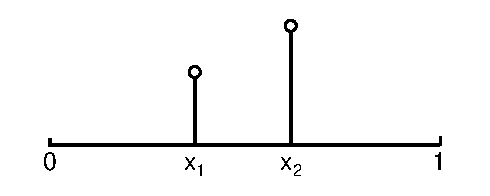
\epsfig{file=mi1.eps}}\end{center}
 
\begin{center}
Fig. 1
\end{center}
 \end{figure}
then there must be at least one local minimum somewhere in the
 range $0 < x < x_2$. Now in this new range, we already have one
 point $(x_1)$, so that a further  reduction in range is possible                                     
 with only one new function evaluation,                                     
  and the procedure can now be continued
with only one new evaluation per stage.
It remains to be shown that this can be continued indefinitely
with a constant reduction in step size, and to calculate what that
reduction will be. Clearly we would get the maximum reduction on the
first step if $x_1$ and $x_2$
were very close together, but we must not forget that
$x_1$ (or $x_2)$ will then be used for the next stage and should therefore be
close to the middle of this new interval as well.  The situation is
illustrated in the figs. 2 and 3, where the distances indicated are
imposed by the symmetry of the intervals and the condition that the
reduction in range must be a factor of $t$ in each stage.  The new range
after evaluation of $F(x_3)$ will be $x_3 < x < x_2$ and
its length must be~$t^{2}$.
 
\begin{figure}
\begin{center}\mbox{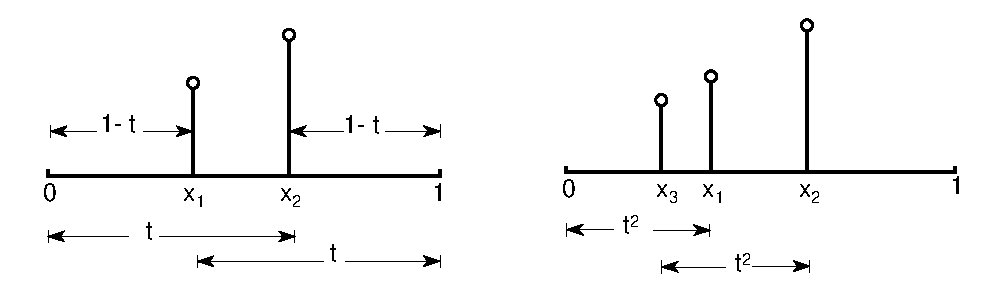
\epsfig{file=mi23.eps,width=.99\textwidth}}\end{center}
 
\begin{center}
Fig. 2\hskip68mm Fig. 3
\end{center}
 \end{figure}
 
This will be possible since there is a real root to the equation:
\begin{eqnarray}
t^2&=&1~-~t\nonumber\\
t&=&{\sqrt{5}~-~1\over
2}~\approx~0.616~.\nonumber
\end{eqnarray}                                  
 
 
Since this ratio $t$ is known as the {\em golden section}, the minimization
technique is called a golden section search.
If the number of stages
to be taken is known in advance, it is possible to improve very slightly
on this technique by using a {\em Fibonacci search}, as described for example
in Kowalik and Osborne \cite{Kowa}.  Although Fibonacci can be shown to be optimal
(in a sense described below), the slight improvement is probably not
worth the added complication.  The golden section search is optimal
among algorithms where the stopping point is not decided in advance.
 
     The above techniques are optimal only in the {\em minimax} sense, that is
they minimize the maximum number of function evaluations necessary to
obtain a given accuracy.  It might be called the pessimist's optimality, 
since in game theory it is the best strategy against an intelligent
opponent who is trying to make you lose.  It should therefore be
effective
in minimizing pathological functions, but in more normal cases we should
expect other methods to be better.  Such methods are described in the
following sections.
 
 
\section{Quadratic interpolation and extrapolation}
 
     A more optimistic approach consists in studying the expected
behaviour of the function and then hoping that the deviations of the
real function from this behaviour are not too great.  From the Taylor's
series analysis of Section 1.5, it would be reasonable to proceed by
assuming that the function is nearly quadratic.
 
     Since a parabola is determined by three points, this method requires
the function to have been evaluated for three different values $x_1, x_2$
and $x_3$. It then predicts the minimum to be at the minimum of the
parabola passing through these points.  If the three function values are
$F_1, F_2,$ and $F_3$, the predicted minimum is at $x_4$ given by
 $$x_4~=~\frac%
      {{\Tstm (x_2~+~x_3)F_1\over\Tstm (x_1~-~x_2)~(x_1~-~x_3)}
  ~+~  {\Tstm (x_1~+~x_3)F_2\over\Tstm (x_2~-~x_1)~(x_2~-~x_3)}
  ~+~  {\Tstm (x_1~+~x_2)F_3\over\Tstm (x_3~-~x_1)~(x_3~-~x_2)}}%
  {2~\left[    {\Tstm F1 \over \Tstm (x_1~+~x_2)~(x_1~-~x_3)}
           ~+~ {\Tstm F_2\over \Tstm (x_2~+~x_3)~(x_2~-~x_3)}
           ~+~ {\Tstm F_3\over \Tstm (x_3~+~x_1)~(x_3~-~x_2)}
    \right]}~. $$ 
Considerable simplification results when the three points are equally
spaced, a distance $d$ apart, in which case:
$$x_4~=~x_2~+~{d\over 2}~{(F_1~-~F_2)\over
(F_1~+~F_3~-~2F_2)}~.$$  
 The function is then evaluated at $x_4$, this point replaces one of the
first three, and a new point is predicted, again by quadratic
interpolation using the new set of three points.
The method terminates when the
predicted function value at some new point agrees with the actual value
within a specified tolerance.
 
     This algorithm usually performs quite well when applied to easy
(nearly quadratic) functions, but suffers from a number of instabilities
which can be quite serious, as follows:
 
  i) At any step the three points may determine a parabola with a maximum
     rather than a minimum, in which case the method diverges.
 
 ii) If the three points lie nearly in a straight line, the algorithm
     takes an enormous step which may cause numerical difficulties as
     well as diverging.
 
iii) After each step there is a choice of which two of the three previous
     points to retain for the next step.  It is usually more convenient
     and logical to retain the most recent points, but this may also lead
     to instabilities by throwing away the best points.
 
 iv) Even without any of the above difficulties, the method may oscillate
     about the minimum instead of converging toward it.
 
     All the problems can be fixed by including checks and safeguards in
the algorithm, but the remedies always involve abandoning, at least
temporarily, the quadratic interpolation step.
The best remedy is probably
to reserve the method for well-behaved functions and to abandon it
entirely as soon as trouble arises.  It is most often used as the last
step in algorithms which depend principally on other methods, since
physical functions are usually quite parabolic in the immediate
vicinity of the minimum.
 
     When derivatives of the function are available, variations of
quadratic interpolation are possible, using instead of three points to
determine the parabola, either two function values and one first
derivative, or the function value and the first two derivatives at one
point. These
variations tend to be even more unstable than the basic method, since
they use information from fewer points.
 
 
\Section{8cm}{The success-failure method}
 
     A good compromise between the stability of the grid search and the
rapid convergence of quadratic interpolation is found with the
success-failure
 technique of Rosenbrock \cite{Rose}.  A start point $x_0$ and initial step size
$d$ are required, and the function is evaluated at $x_0$ and $x_0 + d$.  The first
step is termed a success if $F(x_0 + d)< F(x_0)$, otherwise it is a failure. 
If it is a failure, $d$ is replaced by $-\beta d$, where $\beta$ is a contraction
factor less than one, and the test is repeated.  If it is a success, $x_0$ is
replaced by $x_{0} + d$, $d$ is replaced by $\alpha d$, where  $\alpha$ is an expansion factor
greater than one, and the test is repeated.  The process continues in
this way until the function values change by less than a specified amount,
The numerical values usually used for the expansion and contraction
parameters are $\alpha~\approx~3.0$ and $\beta~\approx~0.4.$
 
     An interesting feature of this method is that a local minimum is
always bracketed whenever a success is followed by a failure.  When this
happens, the middle one of the last three points is always lower than
the outer two, so that one is in a favourable position for trying a
quadratic
interpolation step.  The success-failure method, with one quadratic
interpolation step each time a success is followed by a failure, is
probably
the most effective one-dimensional technique for use on general functions
although in special cases other methods may be superior.
 
\chapter{Stepping Methods in many Variables}
\section{Grid searches and random searches}
 
   An excellent illustration of the enormous increase in complexity in
going to spaces of high dimensionality is afforded by the grid search
technique in many variables. In order to localize a minimum to 1\% of
the range of one variable by this technique requires 100 function
evaluations; in ten variables the number of points required is $10^{20}$.
Clearly we can forget about this method when more than one or
two parameters are involved.
 
In fact it is a general rule in function minimization, as in
function integration, that one should not expect good one-dimensional
techniques to be good when extended to higher dimensionality. Experience
with integration suggests that a {\em Monte Carlo search} is more efficient
than a grid search in many dimensions. The Monte Carlo technique
consists in
choosing points randomly according to some distribution
   (usually uniform or normal).
 
        But even when these methods are refined by using variable search
   ranges, they prove far too slow for general use and we must turn to more
   efficient techniques.
 
 \section{Single-parameter variation}
 
        Since the condition for a minimum which is a stationary point in
  $ n$ variables $x_i$ is the vanishing of all $n$ first derivatives
$\partial F/\partial x_i$, it is
   natural to try to make each derivative vanish separately, one after the
   other.  This is the old method of single
   parameter variation, where one seeks a
   minimum with respect to one\break\hfill
\begin{figure}[t]
\begin{minipage}[b]{.49\textwidth}
\begin{center}\mbox{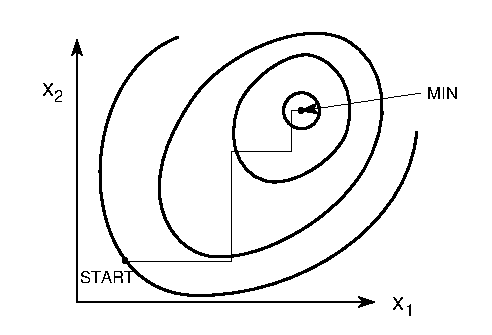
\epsfig{file=mi4.eps,width=.96\textwidth}}\\
Fig. 4
\end{center}
\end{minipage}  \hfill
\begin{minipage}[b]{.49\textwidth}
\begin{center}\mbox{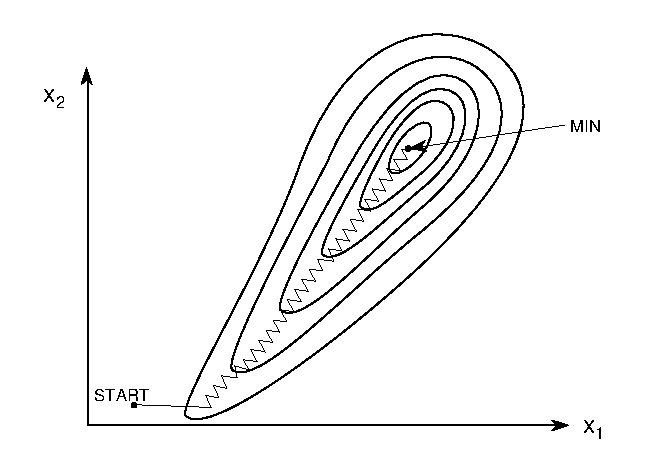
\epsfig{file=mi5.eps,width=.96\textwidth}}\\
Fig. 5
\end{center}
\end{minipage}
\end{figure}
\noindent
 variable at a time using one of the techniques described
 earlier.  Of course when you have finished
 minimizing with respect to $x_2$ you may no
longer be at a minimum with respect to $x_1$,
  so you generally have to start all over
 again, but the process usually does
 converge, as illustrated for two variables in
 fig. 4. Here the curves represent
contours of equal function value, and the straight lines show the steps
taken in minimizing $F$ with respect to $x_1$, then $x_2$, then $x_1$, etc.  In
this case the method converges nicely after only four single-parameter
minimizations.
 
     Consider now the function represented by the contours shown in fig. 5.
Here the method proceeds much more slowly because of the narrow valley. It still converges, but as
the valley becomes narrower, the convergence becomes arbitrarily slow.
 
Such behaviour in many dimensions causes this method to be generally
considered as unacceptably slow.
 
     Two of the more successful improvements aimed at avoiding such
behaviour are due to Hooke and Jeeves \cite{Hook} and Rosenbrock \cite{Rose}.  We discuss
the latter below.
 
 
\section{Rosenbrock's method}
 
     Rosenbrock's algorithm \cite{Rose} starts by performing single-parameter
minimizations as above.  Then when one full cycle of all parameters has
been completed, a new set of orthogonal axes is defined with one axis
taken as the vector from the start point to end point of the cycle.
This vector points in the direction of previous over-all improvement and
is expected to be a good direction for future improvement.  In the case
of the narrow valley seen above, it should point more or less along the
valley and avoid the zig-zag behaviour.  The next cycle of single-variable
 minimizations is performed using multiples of the newly defined
axes as variables.
 
     The Rosenbrock method generally performs well, being quite stable
and capable of following narrow valleys, but as the number of variables
increases, the efficiency drops, probably because the new axis defined
by past improvement is the only `intelligent direction' used in the next cycle. All the other
minimization directions are simply chosen orthogonal to the first one. Also, its terminal
convergence is slow compared with the more `quadratic' methods described in Section 4.
 
 
     Another technique, that of Davies, Swann, and Campey \cite{Dixo} (unpublished,
see Ref. 4) is similar to Rosenbrock's and will not be described here.
 
 
\section{The simplex method}
 
     One of the most successful stepping methods in many variables is
that of Nelder and Mead \cite{Neld}, based on the simplex.  A simplex is an 
$n$-dimensional figure specified by giving its $n$ + 1 vertices.  It is a
triangle in two dimensions, a tetrahedron in three, etc.  The algorithm
takes the name simplex because at each step the information it carries
about the function consists of its values at $n$ + 1 points.  One can
easily visualize how the method works by considering the
two-dimensional
case as in fig. 6.  The three starting simplex points are
somehow  chosen (perhaps randomly) and the function is evaluated at each
point.  Let the point $P_H$ be that at which the function value is highest
(worst) and $P_L$ that at which it is lowest. Let $\bar{P}$ be the centre-of-mass
of all points in the simplex except $P_H$;  that is:
 
 $$\bar{P}~=~{1\over n}\left\{\sum^{n+1}_{i=1}~P_i~-~P_H\right\}~.$$ 
\begin{figure}[t]
\begin{center}\mbox{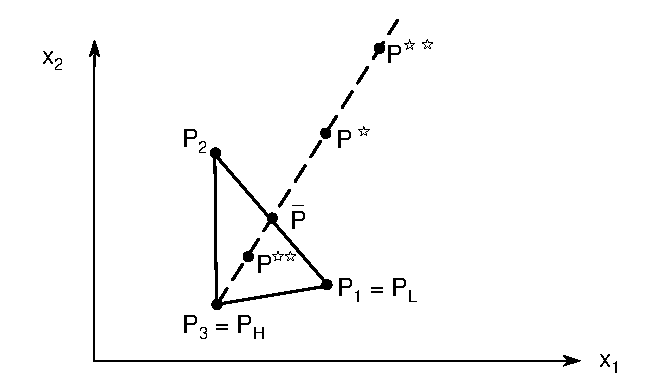
\epsfig{file=mi6.eps}}\end{center}
 
\begin{center}
Fig. 6
\end{center}
\end{figure}
\noindent
From the original simplex, a new simplex is formed by replacing $P_H$ by
a better point if possible.  The first attempt to find a better point is
made by reflecting $P_H$ with respect to $\bar{P}$, producing
$P^* = \bar{P} + (\bar{P} - P_H)$.
If $F(P^*) < F(P_L)$, a new point is tried at $P^{**} = \bar{P} + 2(\bar{P} - P_H)$.  If
$F(P^*) > F(P_H)$, a new point is tried at $P^{**} = \bar{P} - 1/2(\bar{P} - P_H)$.  The best of
the new points then replaces $P_H$ in the simplex for the next step, unless
none of them is better than $P_H$. In the latter case, a whole new simplex
is formed around $P_L$, with dimensions reduced by a factor of 0.5.
 
     Variations on the method are possible by using different contraction
or expansion factors when searching along the line from $P_H$ through $\bar{P}$
(dotted in diagram).  Another interesting possibility is to attempt a
quadratic interpolation step along the dotted line whenever three points
have been determined $(P_H, P^*, P^{**})$.  However, one must be careful not to
accept a point too close to $\bar{P}$, for then the simplex collapses into a line
(or in general a hyperplane of $n - 1$ dimensions) from which it can never
recover.
 
     The simplex algorithm, being designed always to take as big steps
as possible, is rather insensitive to shallow local minima or fine
structure in the function caused by rounding errors, statistical errors
(Monte Carlo output), etc.  Another of its virtues is that of requiring
few function evaluations, usually one or two per iteration.  In addition,
each search is in an `intelligent' direction, pointing from the highest
value to the average of the lowest values.  Compare this with Rosenbrock's
method, where really only the principal axis is an `intelligent' direction,
and all other searches are for exploring along orthogonal axes to
determine a new principal axis.
 
     A convenient convergence criterion for the simplex method is based
on the difference $F(P_H) - F(P_L)$.  The iterations are stopped when this
difference is less than a preset value.  As a final step, the function is
evaluated at $\bar{P}$, which is often slightly better than $F(P_L)$.
 
     In view of the danger mentioned above---of the simplex collapsing
into a hyperplane of dimension $n~-~1$---it has been suggested to use $n~+~2$
or more points rather than $n$ + 1 at each step.  I have tested this idea,
which is equivalent to introducing a dummy parameter of which the
function is independent, and have always found the efficiency of the
algorithm to decrease under these conditions.
 
\section{Conjugate directions method}
 
This method does not require information about the derivatives of the function, 
but the
exploration requires the material
developed in Chapter~\ref{sec:gradmeth}, so it is discussed in 
Section~\ref{sec:conjdir2}.
 
\chapter{Gradient Methods}
\label{sec:gradmeth}
 
\section{Calculating derivatives}
 
     I will call a {\em gradient method} any technique which uses information
from a very small range of the variables (i.e. essentially derivatives)
to predict good trial points relatively far away. This does not necessarily
 mean that they follow the gradient, but only that the gradient, and
perhaps higher derivatives, are used or estimated.
 
     It is of course possible in most cases to calculate analytically the
numerical values of the derivatives of a function, just as it is possible
to calculate the value of the function itseif.  However, it is often
inconvenient and dangerous if the algebra is complicated, so that very
often we are faced with minimizing a function for which no derivatives
are provided. Since the most powerful algorithms discussed below require
derivatives, a general minimization program must be able to estimate the
derivatives of the function by finite differences.
 
     A first derivative may be estimated from
$$\left .{\partial F\over \partial x}\right|_{x_{0}}~\approx~{F(x_0~+~d)~-~F(x_{0})\over
d}~,$$ where $d$ is a `small' displacement.  The error will be, to lowest
order in the Taylor's expansion,
$$\left .\delta~\approx~{d\over 2} \cdot {\partial^{2}F\over \partial x^{2}}\right|_{x_{0}}~.$$
 It is therefore advantageous to make $d$ as small as possible, but still
large enough so that the rounding error in the computation of $F$ does not
become larger than the error introduced by $\delta$. Since the second derivatives may not be known,
it may not be possible to find an optimum step-size $d$, so we may just have to close our eyes and
guess.
 
     A much safer method would be to use points chosen symmetrically
on either side of $x_0$ giving
 $$\left .{\partial F\over \partial x}\right|_{x_{0}}~\approx~{F(x_0~+~d)~-~F(x_0~-~d)\over
2d}~,$$ for in this case the error  $\delta$ vanishes to second order and the lowest
order term is proportional to the third derivative. A disadvantage of
this method is that it requires $2n$ function calls to estimate the $n$ first
derivatives, whereas the asymmetric steps require only $n$ + 1 [or only $n$ if
$F(x_0)$ has to be evaluated anyway].  An advantage of the symmetric steps
method, however, is that it gives the second derivatives as a
by-product [assuming $F(x_0)$ known]:
 
 $${\partial^{2} F\over \partial x^{2}}~\approx~{F(x_0~-~d)~+~F(x_0~+~d)~-~2F(x_{0})\over d^{2}}~,$$
and from the relationship for the error $\delta$ in the asymmetric method,
 a conservative upper limit of the uncertainty in the first derivative
results assuming at least that the symmetric formula gives a smaller
error than the asymmetric one.  A complete treatment of step sizes is
beyond the scope of these lectures but can be found in a paper by
Stewart \cite{Stew}.
 
     The numerical evaluation of second derivatives is facilitated by
the fact that they should be approximately constant over small regions,
so that symmetrical steps are usually not necessary.  Unfortunately,
however, there are a lot of second derivatives to evaluate;  since they
form a symmetric $n~\times~n$ matrix, there are $n(n + 1)/2$ independent
components, requiring at least $n(n - 1)/2$ points  in addition to those
 required for the symmetric derivatives.
\begin{figure}
\begin{minipage}[b]{.49\textwidth}
\begin{center}\mbox{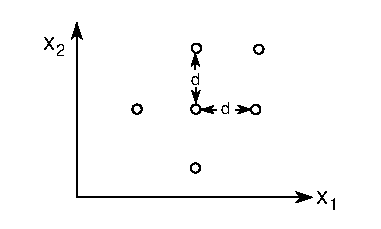
\epsfig{file=mi7.eps}}\\
Fig. 7
\end{center}
\end{minipage} \hfill
\begin{minipage}[b]{.49\textwidth}
\begin{center}\mbox{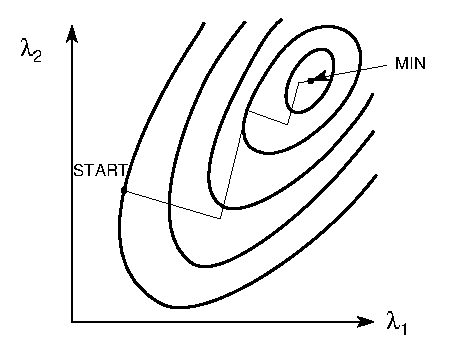
\epsfig{file=mi8.eps}}\\
Fig. 8
\end{center}
\end{minipage} \hfill
\end{figure}
 For two parameters, a minimum
  point pattern is shown fig. 7. The odd point (for
 the mixed second derivative) could
 have been chosen in any corner. The
 two-dimensional diagram is somewhat
 misleading since for large $n$, the
number of `odd points' is $n$ times
  larger than the number of `symmetric' points.
 
\section{Steepest descent}
 
     As soon as the function's first derivatives are known, it is natural
to follow the direction of the negative gradient vector in seeking a
minimum, since this is the direction in which the function is decreasing
the fastest.  Such a technique was used by Cauchy more than a century
ago, and is the basis of what is now known as the method of steepest
descent.
 
     This method consists of a series of one dimensional minimizations,
each one along the direction of local steepest descent (gradient) at the
point where each search begins.  Of course the direction of the gradient
is not constant along a line even for a general quadratic function, so
we expect many iterations to be necessary, but the method can be shown
to converge for a quadratic function. 
 Let us follow its progress
 for a typical function whose contours are shown
 in fig. 8.
   We immediately see an unfortunate
 property of the successive search
 directions: if each linear minimization is exact,
 successive searches must be in orthogonal
directions.  In two dimensions,
this yields steps which look just
like the single parameter variation method (fig. 5) with the axes rotated to
line up with the gradient at the start point.  In many dimensions the
situation is not quite so bad, but successive directions are still
orthogonal and the algorithm cannot be considered acceptable.
\begin{figure}
\begin{center}\mbox{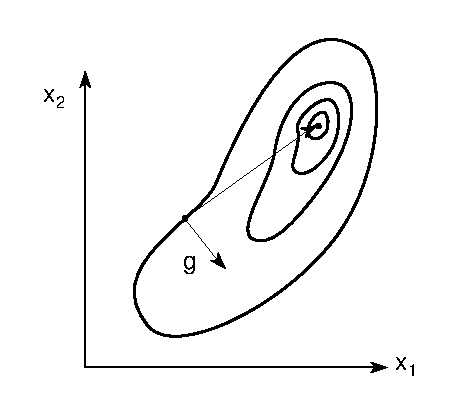
\epsfig{file=mi9.eps}}\end{center}
 
\begin{center}
Fig. 9
\end{center}
\end{figure}
     It is in fact easy to draw contours for a reasonably well-behaved
 hypothetical function (fig. 9)
 where the direction to the
 minimum is just perpendicular to the gradient.
 
\section{Newton's method}
 
     It is clear that since a general quadratic function is determined
by specifying its value, first derivatives, and second derivatives at a
point, it can be minimized in one step if and only if all this information
(or its equivalent) is taken into account.  Let us write a
quadratic function as
 $$F({\underline{x}})~=~F({\underline{x}}_0)~+~{\underline{g}}^T 
({\underline{x}}~-~{\underline{x}}_0)~+~{1\over 2}~({\underline{x}}~-~{\underline{x}}_0)^T~\UTG
   ({\underline{x}}~-~{\underline{x}}_0)~,$$
 where the gradient ${\underline{g}}$ is evaluated at ${\underline{x}}_0$ and the second derivative
matirx $\UTG$is a constant.  Then the minimum is given directly by
 
                     $${\underline{x}}_m~=~{\underline{x}}_0~-~\UTG\!\!^{-1}{\underline{g}}~=~
{\underline{x}}_0~-~\UTV{\underline{g}}~,$$
 where the inverse of the second derivative matrix is the {\em covariance
matrix} $\UTV$.
 
     This is then the many-dimensional equivalent of quadratic
interpolation
discussed earlier, and it is subject to the same sort of difficulties
when applied as an iterative technique to general non-quadratic functions.
But let us first point out its good features:
 
  i) the step size is no longer arbitrary, but is prescribed precisely by
     the method;
 
 ii) the step directions are no longer necessarily along the gradient
     vector but take account of parameter correlations (narrow valleys
     or ridges) through the mixed second derivative terms.
 
     In practice, however, the method is unstable, essentially for the
reasons given in Section 2.4.  In particular, it diverges whenever the
matrix $\UTG$ (or $\UTV$) is not positive-definite (see next section).  In its
unmodified form  the method is used only when the minimum is known to
be very close or when the function is known to be positive quadratic (for
linear least squares).  However, it is clearly a powerful technique
and is worth studying in some detail since all the most successful
algorithms are based on {\em Newton-like steps}, as discussed below.
 
\section{Positive-definite quadratic forms}
 
     We pause here briefly to consider the properties of quadratic forms
useful for understanding the more powerful gradient methods.  In one
dimension the description is simple;  a general quadratic form can be
written
  $$F(x)~=~a~+~gx~+~{1\over 2}~Gx^2~, $$
 where $g = \partial F/\partial x$ at $x$ = 0, and $G = \partial^2 F/\partial x^2$ also at $x$ = 0.
This function
has a minimum if and only if $G \ge$ 0.  If $G$ = 0, the minimum is at infinity,
The minimum (if it exists) is at $x = -g/G$.  When using a quadratic
approximation to minimize a general non-linear function, it makes sense to
take a step to $x = -g/G$ only if $G > 0$ since otherwise we step to
a predicted maximum or to infinity.  A possible remedy if $G < 0$ is to
take a
step $x = -g$;  that is, to set $G$ arbitrarily equal to unity so that the
step will at least be in the right direction although it will now have
arbitrary length.  Consideration of fig. 10 shows that this is
the only thing we can do unless more information is available, since the
quadratic part of the function is not {\em convex} or {\em positive-definite} at
the point $x_0$.
 
\begin{figure}
\begin{minipage}[b]{11cm}
\begin{center}\mbox{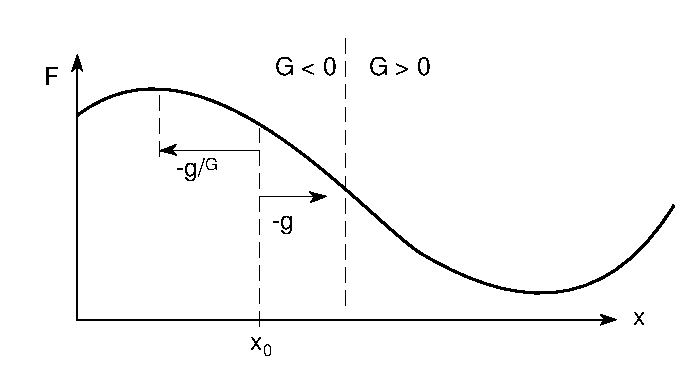
\epsfig{file=mi10.eps,width=108mm}}\\
Fig. 10
\end{center}
\end{minipage} \hfill
\begin{minipage}[b]{49mm}
\begin{center}\mbox{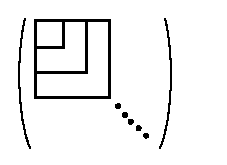
\epsfig{file=mi11.eps,width=48mm}}\\[5mm]
Fig. 11
\end{center}
\end{minipage}
\end{figure}
      These arguments may now be extended to many dimensions where $g$
becomes the gradient vector ${\underline{g}}$, and $G$ becomes the second derivative matrix
$\UTG$. Then the Newton step to ${\underline{x}} = -\UTG\!\!^{-1}{\underline{g}}$ makes sense 
only if $\UTG$
 (hence $\UTG\!\!^{-1})$ is a positive-definite matrix, since only then does the quadratic form
 $$F({\underline{x}})~=~a~+~{\underline{g}}^T \cdot {\underline{x}}~+~{1\over 2}~{\underline{x}}^T
\UTV {\underline{x}}$$
have a minimum.  If $\UTG$ is singular, the predicted minimum (or maximum)
is not unique.
 
     Unfortunately there is no simple way of telling, in general, if a
matrix is positive-definite by inspecting individual components, but we
can at least state some of the many useful properties of such matrices.
Two necessary (but not sufficient) conditions for a (square, symmetric)
matrix to be positive-definite are:
 
  i) the diagonal elements must be positive (this is in fact sufficient
     for a 1 $\times$~1 matrix);
 
 ii) the off-diagonal elements must obey $G^2_{ij} < G_{ii}G{jj}~.$
 
[Properties (i) and (ii) together are sufficient for a 2 $\times$ 2 matrix.]
While the above conditions are easy to check, they are not in general
sufficient.  Some necessary {\em and} sufficient conditions are the following:
 
 iii) All the eigenvalues of the matrix are positive. This is generally
      a rather difficult calculation and is usually approximate.
 
 iv) The determinants of all the upper left square submatrices (formed
     as indicated in the diagram in fig. 11) are
     positive.  This is probably the easiest method.
 
  v) The scalar ${\underline{e}}^T \UTG{\underline{e}}$ is positive for all vectors
${\underline{e}}$  This is usually
     taken as the definition of a positive-definite matrix, and explains
     why a positive-definite matrix yields a quadratic form with a
     minimum:  the function increases in all directions from ${\underline{e}}~=~0$.
 
 vi) The inverse $\UTG\!\!^{-1} = \UTV$ is positive-definite.
 
     Now suppose that $\UTG\!\!^{-1}$ is calculated for a Newton  step and turns out
to be non-positive-definite.  In analogy to the one dimensional case we
would simply take $\UTG = \UTI$, the unit matrix, and the Newton step would
become a steepest-descent step of arbitrary length, which is probably
not so bad an idea and is in fact often done.  But we can do better by
trying to make a positive-definite matrix which is as `close' as possible
to the unacceptable $\UTG$. This is done as follows:
 The matrix $(\UTG + \lambda \UTI)^{-1}$ is
used instead of $\UTG\!\!^{-1}$, where $\lambda$ is greater
     than the largest negative eigenvalue of $\UTG\!.$  This requires a fair
     amount of calculation and so is not very convenient, but it is
     quite appealing since it amounts to taking a step which is intermediate between a Newton step
and a steepest-descent step (for
     large values of  $\lambda$ the step becomes short and in the direction of
     the gradient).
 
 If we are willing to calculate eigenvectors as well as eigenvalues, the
     non-positive-definiteness can be turned into an advantage, since the eigenvector
corresponding to a negative eigenvalue
     indicates a direction (or directions) in which the negative first
     derivative is {\em increasing} in magnitude rather than decreasing.  This
     suggests an especially fruitful direction for a
single-parameter-variation step which should not only lead to a good
decrease of the
     function value but should also lead more quickly to a region of
     positive-definiteness.
 
     Minimization methods based on variations of Newton's method as
suggested by the above considerations are usually called quasi-Newton
methods.  Many such algorithms have been published and some are quite
successful, but the field is still open for new ideas.
 
     The principal drawback of such techniques is the repeated evaluation
 and inversion of the second-derivative matrix.  The calculation of
the second derivatives usually requires a rather long time, proportional
to $n^2$, and the matrix inversion, although usually faster, increases with
$n$ like $n^3$.
 
     One of the most interesting results concerning quadratic forms is
the basis of a collection of related techniques described in the next
sections, which do not require explicit repeated evaluations of $\UTG$.
 
 
\section{Conjugate directions}
\label{sec:conjdir2}
 
     The vectors ${\underline{d}}_i$ and ${\underline{d}}_j$ are said to be {\em conjugate} with
respect to a positive-definite symmetric matrix $\UTA$ if
 
 $${\underline{d}}^T_i \UTA{\underline{d}}_j~=~0\qquad {\rm for}\qquad i \neq j~.$$
 
If $\UTA$ is the unit matrix $\UTI$, the conjugate vectors $\UTd$ would be orthogonal,
so conjugacy can be thought of as a generalization of orthogonality. A
set of $n$ conjugate vectors span an $n$-dimensional space, and any point
in the space can therefore be expressed as a linear combination of $n$
conjugate vectors.
 
     Although the matrix $\UTA$ does not uniquely define a set of conjugate
vectors, such a set can always be constructed by a procedure similar to
the Gram-Schmidt orthogonalization method.  Let us start for example
with an arbitrary vector ${\underline{d}}_1$.  Then the vector
 
 $${\underline{d}}_2~=~\UTA{\underline{d}}_1~-~{{\underline{d}}^T_1
\UTA\UTA{\underline{d}}_1\over {\underline{d}}^T_1 \UTA{\underline{d}}_1}~{\underline{d}}_1$$
can be seen to be conjugate to ${\underline{d}}_1$ since the product ${\underline{d}}^T_1 \UTA
{\underline{d}}_2$ vanishes
identically.  The process can then be continued in the same way to
construct a ${\underline{d}}_3$ which will be conjugate to both ${\underline{d}}_1$ and 
${\underline{d}}_2$,
and so forth up to ${\underline{d}}_n$.
 
     Such vectors become interesting for minimization problems when they
are conjugate with respect to the hessian (second derivative) matrix $\UTG$.
In this case a theorem of Fletcher and Reeves \cite{Flet1} states that a sequence
of linear minimizations in each of the $n$ conjugate directions will
minimize a general quadratic function of $n$ variables.  That this is true
can be seen quite easily as follows.  Let the quadratic function be
 $$F({\underline{x}})~=~F({\underline{0}})~+~{\underline{g}}^T {\underline{x}}~+~{1\over 2}~
{\underline{x}}^T \UTG\!{\underline{x}}$$
 and the $n$ directions $d_i$ be conjugate with respect to $\UTG$:
             $${\underline{d}}_i^T\UTG{\underline{d}}_j~=~0~,\qquad i\neq j~.$$
Then the vectors ${\underline{x}}$ and ${\underline{g}}$ can be expressed as linear combinations
\begin{eqnarray}
{\underline{x}}&=&\sum_{i}~y_i{\underline{d}}_i\nonumber \\
\nonumber\\
{\underline{g}}&=&\sum_{i}~c_i{\underline{d}}_i~,\nonumber
\end{eqnarray}
so that the general quadratic becomes
 $$F({\underline{x}})~=~F({\underline{0}})~+~\left(\sum_i~c_i{\underline{d}}^T_i\right)
\left(\sum_j~ y_j{\underline{d}}_j\right)~+~{1\over 2}~\left(\sum_i~y_i{\underline{d}}^T_i\right)
\UTV~\left(\sum_j~ y_j{\underline{d}}_j\right)~.$$
 Now  if the last term above is regrouped as a double sum, the terms with
 $i\neq j$  drop out because of the conjugacy condition, so that the whole
expression can be simplified as
 \begin{eqnarray}
F({\underline{x}})&=&F({\underline{0}})~+~\sum_i~\sum_j~c_i{\underline{d}}^T_i
{\underline{d}}_j y_j~+~{1\over
2}~\sum_{j}~y^2_j{\underline{d}}^T_j\UTG{\underline{d}}_j\nonumber\\
&=&F({\underline{0}})~+~\sum_j~\left(b_j y_j~+~b^{\prime}_j y^{2}_j\right)\nonumber
\end{eqnarray}
where
 $$b_j~=~\sum_i~c_i{\underline{d}}^T_i{\underline{d}}_j$$
 and
 $$b^{\prime}_j~=~{\underline{d}}^T_j \UTG{\underline{d}}_j$$
 are constants. By expressing the quadratic in terms of $y$ instead of $x$
we have separated it into a sum of independent one-parameter quadratic
functions.  A minimization with respect to $y_i$ (a linear minimization
along the direction ${\underline{d}}_i$) will therefore be independent of the minimizations
along the other conjugate directions, which demonstrates the validity
of the theorem.
 
     The above theorem tells us what is `wrong' with the
single-parameter-va\-ria\-tion method:  we should
be using conjugate directions rather than
simply orthogonal axes.  However, since the construction of conjugate
vectors seems to require knowledge of the hessian $\UTG$, this does not yet
help very much in practice, for if we knew $\UTG$ (and ${\underline{g}}$) we could minimize
a quadratic immediately by means of Newton's method, and would not need
to use $n$ linear minimizations.
 
     The usefulness of conjugate directions comes from the fact that
there are ways of determining such directions implicitly, without first
evaluating the entire hessian matrix $\UTG$.  Of course, by the time all $n$
conjugate directions are determined, by whatever method, information
equivalent to the matrix $\UTG$ must have been determined.  However, by that
time considerable minimization may already have been performed, as in
the method implied by the following theorem.
 
If ${\underline{x}}_0$ and ${\underline{x}}_1$ are minimum points in two parallel subspaces, then
the direction 
\begin{figure}
\begin{center}\mbox{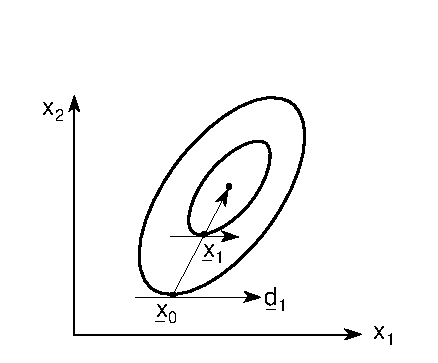
\epsfig{file=mi12.eps}}\end{center}
 
\begin{center}
Fig. 12
\end{center}
\end{figure}
${\underline{x}}_1-{\underline{x}}_0$
is conjugate to any vector which lies in either
 subspace. This can easily be seen in
two dimensions as illustrated
in  fig. 12. Since ${\underline{x}}_0$
 is a minimum along the direction ${\underline{d}}_1$
 the gradient of $F$ at ${\underline{x}}_0$ must be
 orthogonal to ${\underline{d}}_1$:
$${\underline{d}}^T_1({\underline{g}}~+~\UTG
{\underline{x}}_0)~=~0~,$$ 
where ${\underline{g}}$ is the gradient at ${\underline{x}} = {\underline{0}}$.  
Similarly at ${\underline{x}}_1$:
$${\underline{d}}^T_1({\underline{g}}~+~\UTG
{\underline{x}}_1)~=~0~.$$
Subtracting the above equations, the first terms drop out and we have:
 $${\underline{d}}^T_1 \UTG({\underline{x}}_1~-~{\underline{x}}_0)~=~0~,$$
showing that $({\underline{x}}_1~-~{\underline{x}}_0)$ is conjugate to ${\underline{d}}_1$.
 
     Unfortunately, extending this algorithm to three dimensions requires
three additional minimizations in order that the third direction be
conjugate to both of the first two, so that convergence for a general
quadratic in $n$ variables is obtained only after $n$ iterations involving in
all $n(n$ + 1)/2 linear minimizations.  Since this is just the number of
independent elements in the second derivative matrix, we would be better
off for quadratic functions to calculate this matrix directly and avoid
the linear searches.  On the other hand, for non-quadratic functions the
conjugate directions method should be much more stable since it proceeds
by a series of linear searches in independent directions and still
guarantees convergence in a finite number of steps once a quadratic
region is entered.  In addition, this method has the advantage of
requiring neither first nor second derivatives of the function.
(Strictly speaking, then, it should have been discussed in Section 3
rather than in this section.)
 
      A disadvantage of the algorithm described above is that for each
iteration, $n$ minimizations are performed in direction ${\underline{d}}_1$, whilst only
one is performed in direction ${\underline{d}}_n$.  This undesirable asymmetry is largely
avoided in a variation due to Powell \cite{Powe1}.
 
\section{Conjugate gradients}
 
      When the first derivatives of the function are calculated, a somewhat
more elegant method can be used, known as the method of {\em conjugate
gradients} \cite{Flet1}. Suppose that the function and its gradient are evaluated
at two points ${\underline{x}}_0$ and ${\underline{x}}_1$, giving differences:
 \begin{eqnarray}
{\underline{\Delta}}{\underline{x}}&=&{\underline{x}}_1~-~{\underline{x}}_0\nonumber\\
{\underline{\Delta}}{\underline{g}}&=&{\underline{g}}_1~-~{\underline{g}}_0~.\nonumber
\end{eqnarray}
Then if the function were quadratic with hessian $\UTV$ we would have
 $${\underline{\Delta}}{\underline{g}}~=~\UTG~ {\underline{\Delta}}{\underline{x}}~.$$
Any vector ${\underline{d}}_1$ orthogonal to ${\underline{\Delta}}{\underline{g}}$
 would then be conjugate to ${\underline{\Delta}}{\underline{x}}$:
 $${\underline{d}}^T_1~{\underline{\Delta}}{\underline{g}}~=~
{\underline{d}}^T_1~\UTG~{\underline{\Delta}}{\underline{x}}~=~0~,$$
 which immediately suggests a method for obtaining conjugate directions
without knowing $\UTG$, based on the change in gradient along a previous
direction.
 
     In the method of conjugate gradients, successive one-dimensional
minimizations are performed along conjugate directions with each direction being used only once per iteration.  The first direction is taken
as ${\underline{d}}_0 = -{\underline{g}}_0$, the steepest descent vector at ${\underline{x}}_0$. 
Let the minimum along this direction be at ${\underline{x}}_1$ where the gradient is
${\underline{g}}_1$.  Then the next  search direction ${\underline{d}}_1$, which we want to be
conjugate to ${\underline{d}}_0$ must be a linear combination of the only vectors we have at hand,
namely:
 $${\underline{d}}_1~=~-{\underline{g}}_1~+~b{\underline{d}}_0~.$$
The conjugacy condition is
 $${\underline{d}}_1^T\UTG{\underline{d}}_0~=~{\underline{d}}_1^T\UTG({\underline{x}}_1~-~
{\underline{x}}_0)~=~0$$
or
$$(-{\underline{g}}_1^T~+~b{\underline{d}}_0^T)\UTG{\underline{d}}_0~=~
(-{\underline{g}}_1^T~-~b{\underline{g}}_0^T)({\underline{g}}_1~-~{\underline{g}}_0)~=~0~.$$
Since ${\underline{x}}_1$ is a minimum along direction ${\underline{d}}_0 = -{\underline{g}}_0$, the
direction ${\underline{g}}_0$ is orthogonal to the gradient at ${\underline{x}}_1$,
 so that ${\underline{g}}_1^T{\underline{g}}_0 = 0$.  We are then left with
 $$b~=~{{\underline{g}}_1^T{\underline{g}}_1\over {\underline{g}}_0^T{\underline{g}}_0}$$
 so that the new conjugate direction is
 $${\underline{d}}_1~=~-{\underline{g}}_1~+~\left(
{{\underline{g}}_1^T{\underline{g}}_1\over {\underline{g}}_0^T{\underline{g}}_0}\right)~
{\underline{d}}_0~.$$ 
This process can be continued to generate $n$ directions, each one conjugate
to all the others.  It turns out that the same simple formula holds
for all the successive conjugate directions
 $${\underline{d}}_{i+1}~=~-{\underline{g}}_{i+1}~+~\left(
{{\underline{g}}_{i+1}^T{\underline{g}}_{i+1}\over {\underline{g}}_i^T{\underline{g}}_i}\right)~
{\underline{d}}_i~.$$ 
 
\section{Variable metric methods (VMM)}
 
     In analogy with the methods of differential geometry and general
relativity, it is convenient to consider the properties of the function
$F({\underline{x}})$ as being in fact properties of the space of the variables ${\underline{x}}$.
 We have already made some rudimentary use of this idea when we generalized
from the usual orthogonal coordinate axes to a system defined by axes
pointing in conjugate directions.  We now wish to go further and be able
to express the properties of the function $F$ geometrically as the properties 
of the non-Euclidean space of its variables ${\underline{x}}$.
 
     The fundamental invariant in a non-Euclidean space is the squared
distance element
 $$ds^{2}~=~{\underline{d}}{\underline{x}}^T\UTA{\underline{d}}{\underline{x}}~,$$
 where ${\underline{d}}{\underline{x}}$ is a differential coordinate displacement and $\UTA$ is
the {\em covariant
metric tensor} which determines all the properties of the space under
consideration. When $\UTA$ is just the unit matrix $\UTI$, the above formula for
$ds^2$ just expresses the Pythagorean theorem for an $n$-dimensional
Euclidean
space. When off-diagonal elements of $\UTA$ are non-zero and when the
elements are allowed to vary as functions of ${\underline{x}}$, a generalized
non-Euclidean space is generated.
 
     It is easily verified that the second derivative (hessian) matrix $\UTG$
behaves under coordinate transformations like a covariant tensor and
we will identify it with the metric tensor of our space.  The inverse
$\UTV = \UTG\!\!^{-1}$ is a contravariant tensor and becomes the contravariant metric
tensor.  (For a discussion of covariant and contravariant tensors, see
for example chapter 10 of Ref. [9].)  This immediately enables us to
construct two scalar (invariant under coordinate transformations)
quantities:
$$a)\qquad ds^2~=~ {\underline{d}}{\underline{x}}^T\UTG{\underline{d}}{\underline{x}}$$
is the square of the generalized distance between the point ${\underline{x}}$ and the
point ${\underline{x}} + {\underline{d}}{\underline{x}}$.  When $F$ is a chisquare
 function which is minimized to
determine some best parameters ${\underline{x}}$, then the physical meaning of the
generalized distance $ds$ is just the number of `standard deviations'
 ${\underline{x}} + {\underline{d}}{\underline{x}}$ is away from ${\underline{x}}$.  
That is, the use of the metric tensor $\UTV$
enables
us to scale the distance ${\underline{d}}{\underline{x}}$ so that it comes out as a physically (or
statistically) meaningful invariant quantity instead of being expressed
in arbitrary units (or a mixture of arbitrary units!).
\vskip2mm \noindent
And{\phantom{xxxxxxxxxxxxxxxxxxx}} $b)\qquad \rho~=~{\underline{g}}^T\UTV{\underline{g}}$\\
\vskip2mm
\noindent
 is twice the difference between the function value at the point where $\UTV$
and the gradient ${\underline{g}}$ are calculated and the minimum of a quadratic form
with hessian matrix  $\UTG = \UTV\!\!^{-1}$.  That is, $\rho$/2 is the expected (vertical)
distance to the minimum if the function $F$ were quadratic. This provides
us with an important scale-free {\em convergence criterion} for any method
which provides approximations to $\UTV$ and ${\underline{g}}$.
 
     When the function $F$ is quadratic, $\UTG$ is constant everywhere and, in
the sense outlined above, this is equivalent to working in a space with
a constant metric.  For real non-linear functions we expect higher-order
terms to be small but not negligible, so that we can think of working in
a space with a slowly-varying metric tensor. Minimization methods based
on this approach are known as {\em variable metric methods}.  They differ from
the basic Newton-Raphson method in that the matrix $\UTG$ is not
completely
re-evaluated at each iteration, but is assumed to be well approximated by
taking the $\UTG$ of the previous iteration and applying a correction based on
new information from the current iteration.  This correction is known as
the {\em matrix updating formula}, which in general differs from method to
method.
 
     Variable metric methods therefore proceed generally by the following
steps:
 
  i) A starting point ${\underline{x}}_0$ is given, the gradient ${\underline{g}}_0$ at that point is
     calculated, and some approximation to  $\UTG\!\!^{-1}$, say $\UTV\!\!_0$, is constructed.
     The starting $\UTV\!\!_0$ may be only the unit matrix, or it may actually be
     the inverse of the full second derivative matrix.
 
 ii) A step is taken to ${\underline{x}}_1 = {\underline{x}}_0 - \UTV\!\!_0
{\underline{g}}_0$, which would be the
minimum if $F$
     were quadratic and if $\UTV\!\!_0$ were the true covariance matrix.  Since ${\underline{x}}_1$
     is not the position of the minimum in the general case, it is usual
     to perform a linear search along this direction, finding the $\alpha$
     which minimizes $F({\underline{x}}_0 - \alpha\UTV{\underline{g}}_0)$.  In either case let the
new point be
     called ${\underline{x}}_1$ and let the gradient calculated at ${\underline{x}}_1$ 
be ${\underline{g}}_1$.
 
iii) The matrix $\UTV$ is corrected using an updating formula of the form
 $$\UTV\!\!_1~=~\UTV\!\!_0~+~\UTf(\UTV\!\!_0,{\underline{x}}_0,
{\underline{x}}_1,{\underline{g}}_0, {\underline{g}}_1)~.$$
     Then ${\underline{g}}_0$ is replaced by ${\underline{g}}_1,~ {\underline{x}}_0$ by
${\underline{x}}_1$, and $\UTV\!\!_0$ by $\UTV\!\!_1$, and steps (ii)
     and (iii) are repeated until some convergence criteria are satisfied.
 
     The different methods differ chiefly in the choice of updating
function $\UTf$, as described in the following sections, and in the extent to
which linear minimizations are necessary.  Less important variations
involve the starting approximation $\UTV\!\!_0$ and various safeguards against
`unreasonable' steps and non-positive-definiteness as for the Newton
techniques.
 
 
\section{Davidon's rank-two formula}
 
     Probably the first---and perhaps still the best---variable metric
method was developed in 1959 by Davidon and later published in simplified
form in 1963 by Fletcher and Powell \cite{Flet}.  Davidon's updating formula for
the covariance matrix is the following:
 
$$\UTV\!\!_1~=~\UTV\!\!_0~+~{{\underline{\delta}}{\underline{\delta}}^T\over {\underline{\delta}}^T
{\underline{\gamma}}}~-~{~\UTV\!\!_0{\underline{\gamma}}{\underline{\gamma}}^T~\UTV\!\!_0\over
 {\underline{\gamma}}^T\UTV\!\!_0{\underline{\gamma}}}~,$$
where the changes in position and gradient on the last step were
 $${\underline{\delta}}~=~{\underline{x}}_1~-~{\underline{x}}_0$$
and
$${\underline{\gamma}}~=~{\underline{g}}_1~-~{\underline{g}}_0~,$$
 and $\UTV\!\!_0$ was the previous estimate of the covariance matrix.  This is
called a rank-two formula since the correction $\UTV\!\!_1 - \UTV\!\!_0$ is a matrix of
rank two in the space of $\delta$ and $\UTV\!\!_0{\underline{\gamma}}$ as can be seen directly by
inspection of the formula.
 
     One fundamental requirement of an updating formula is that the new
matrix satisfies the relationship
 $$\UTV\!\!_1{\underline{\gamma}}~=~{\underline{\delta}}~,$$
since ${\underline{\gamma}}~=~\UTG{\underline{\delta}}$ for a quadratic with hessian $\UTG$. 
 It is easily seen that Davidon's formula satisfies this requirement:
\begin{eqnarray}
\UTV\!\!_1{\underline{\gamma}}&=&\left[\UTV\!\!_0~+~{\delta\delta^T\over \delta^T\gamma}~-~
{\UTV\!\!_0{\underline{\gamma}}{\underline{\gamma}}^T\UTV\!\!_0\over {\underline{\gamma}}^T 
\UTV\!\!_0{\underline{\gamma}}}\right]~{\underline{\gamma}}\nonumber \\
&=&\UTV\!\!_0{\underline{\gamma}}~+~{{\underline{\delta}}{\underline{\delta}}^T{\underline{\gamma}}
\over {\underline{\delta}}^T{\underline{\gamma}}}~-~
{\UTV\!\!_0{\underline{\gamma}}{\underline{\gamma}}^T\UTV\!\!_0{\underline{\gamma}}\over
{\underline{\gamma}}^T\UTV\!\!_0{\underline{\gamma}}}\nonumber \\
&=&\UTV\!\!_0{\underline{\gamma}}~+~
{\underline{\delta}}~-~\UTV\!\!_0{\underline{\gamma}}~=~
{\underline{\delta}}~.\nonumber
\end{eqnarray}
 
  An unfortunate feature of the Davidon algorithm is the need to
perform at each iteration a linear minimization along the direction
given by a Newton step, $-\UTV{\underline{g}}.$  This linear search step is, however,
necessary in order to assure convergence for general functions. Fletcher
and Powell show \cite{Flet} that if the starting approximation to $\UTV$ is
positive-definite, then
$\UTV$ will remain positive-definite after all updatings, but
they have to use the fact that each iteration is a linear minimization,
that is
$${\underline{g}}^T_1\UTV\!\!_0{\underline{g}}_0~=~0~.$$
 
     It can be shown that this method is quadratically convergent, at
most $n$ iterations ($n$ linear searches and $n$ gradient calculations) being
required for an $n$-dimensional quadratic form.
 
 
\section{The rank-one formula}
 
     In an effort to avoid the linear minimizations required by Davidon's
algorithm, several workers have independently developed an interesting
updating formula of rank one.  In this case Davidon in 1968 was the
first
to publish an algorithm \cite{Davi} based on the formula, and Powell \cite{Powe2} has
summarized the properties of this formula and of algorithms based on it
 
     The rank-one updating is:
$$\UTV\!\!_1~=~\UTV\!\!_0~+~{({\underline{\delta}}~-~\UTV\!\!_0{\underline{\gamma}})
({\underline{\delta}}~-~\UTV\!\!_0{\underline{\gamma}})^T\over
{\underline{\gamma}}^T({\underline{\delta}}~-~\UTV\!\!_0{\underline{\gamma}})}~.$$
It can be shown \cite{Powe2} that this is the only formula of rank two (or less)
for which not only $\UTV\!\!_1{\underline{\gamma}} = \delta$ but:
$$\UTV\!\!_1{\underline{\gamma}}_i~=~{\underline{\delta}}_i~,$$
 where ${\underline{\delta}}_i$ and ${\underline{\gamma}}_i$ are the step
 and gradient changes at {\em any} previous
iteration.  This is known as the {\em hereditary property}, since $\UTV\!\!_1$ can be
said to
inherit the fundamental property $\UTV{\underline{\gamma}} = {\underline{\delta}}$  with respect
to all previous iterations (up to $n$).
 
     The hereditary property assures that after $n$ iterations, $\UTV\!\!_1$ will be
the true covariance matrix if $F$ is quadratic, no matter what steps were
taken (almost), so that if Newton steps are taken, convergence for a
quadratic function is assured after $n$ iterations, without the need for
linear minimizations.
 
     In addition, the rank-one formula is {\em symmetric}, in the sense that
the expression for $\UTV\!\!_1^{-1}$ in terms of $\UTV\!\!_0^{-1}$ is the same as that for
$\UTV\!\!_1$ in terms of $\UTV\!\!_0$ provided ${\underline{\delta}}$ and ${\underline{\gamma}}$ are
interchanged. The meaning of this symmetry property will be discussed in the next section.
 
     But, as nothing is perfect, so the elegance and mathematical beauty
of the rank-one formula hide a number of numerical and practical difficulties which can make it highly unstable when applied to a general
function.  In particular, if the vector ${\underline{\gamma}}$ happens to be orthogonal to the
vector $({\underline{\delta}}- \UTV\!\!_0{\underline{\gamma}})$, the denominator goes to zero in
the updating formula, and an unbounded correction is possible.  Since these vectors may be
orthogonal, even for a quadratic function, the problem of numerical
instability is a serious one.
 
     Moreover, the matrices $\UTV\!\!_1$ do not really converge to the true covariance matrix 
in the usual meaning of the term convergence.  Although
it is true that $\UTV\!\!_1$ will be equal to the true covariance matrix at the
$n^{\rm th}$ step for a quadratic function (barring numerical difficulties), the
intermediate matrices $\UTV$ may vary wildly from step to step, so that on
any particular iteration $\UTV\!\!_1$ may be a rather poor approximation.  This is
especially dangerous when the function is not quadratic, since the large
corrections necessary in later iterations will generally not compensate
properly the fluctuations in early steps.  Also, there is no guarantee
that intermediate matrices will remain positive-definite, and hence no
guarantee of a reduction in the value of $F$ at each step, even for a
quadratic $F$.
 
     All these difficulties can, of course, be overcome by programming
enough safeguards into the algorithm, but this can only be done at the
expense of efficiency and sometimes only by abandoning temporarily the
updating formula itself, which makes it lose some of its appeal.\\ \noindent
Different approaches are possible depending on whether it is considered
important to maintain positive definiteness as in the Davidon
algorithm \cite{Davi}, or important not to abandon the exact rank-one formula
as in Powell's method \cite{Powe2}.
 
 
\section{Fletcher's unified approach to VMM}
 
     The existence of two different updating formulas with very different
properties generated a lot of interest in variable metric methods (VMM)
during the years 1967--1971, since it showed VMM to be very promising
and left many questions unanswered, such as:
 
  i) How can it be that the rank-one and rank-two formulas have such
     different properties?  What is the relationship between them?
 
 ii) Is there a way to combine the best properties of both formulas?
 
iii) Are there other good formulas?  Is it possible to define a class
     of `admissible' formulas?
 
     A certain understanding of the above problems has recently been
made possible by the work of a number of people. In particular, a 
paper by Fletcher \cite{Flet2} presents a unified approach to VMM, which will be
given here.
 
     Recall that the rank-one equation is symmetrical (in a sense defined
in Section 4.9), but as we shall now see, the rank-two formula is not.
Indeed the asymmetry suggests a way to construct a possible third
formula
by taking the `mirror image' of the rank-two formula.  The basic idea is
that a new formula should satisfy the fundamental relationship
 $$\UTV\!\!_1{\underline{\gamma}}~=~{\underline{\delta}}~,$$
 and therefore its inverse should satisfy
 $${\underline{\gamma}}~=~\UTV\!\!_1^{-1}{\underline{\delta}}~.$$
 We can indeed write down the updating formula for $\UTV\!\!_1^{-1}$ which
corresponds to the rank-two formula for $\UTV\!\!_1$:
 $$\UTV\!\!_1^{-1}~=~\left(\UTI~-~{{\underline{\gamma}} {\underline{\delta}}^T\over
{\underline{\delta}}^T{\underline{\gamma}}}\right)
\UTV\!\!_0^{-1}~\left(\UTI~-~{{\underline{\delta}} {\underline{\gamma}}^T\over
{\underline{\delta}}^T{\underline{\gamma}}}\right)~+~
{{\underline{\gamma}}{\underline{\gamma}}^T\over
{\underline{\delta}}^T{\underline{\gamma}}}~.$$
This matrix $\UTV\!\!_1^{-1}$ can now be thought of as a mapping
from  ${\underline{\delta}}~\to~{\underline{\gamma}}$ since ${\underline{\gamma}} = \UTV\!\!_1^{-1}
{\underline{\delta}}$.  If we interchange ${\underline{\gamma}}$ and ${\underline{\delta}}$ 
in the formula, it
will then give a mapping from ${\underline{\gamma}} \to {\underline{\delta}}$, thereby
 producing a new updating formula
where $\UTV\!\!_1{\underline{\gamma}} = {\underline{\delta}}$.  The new {\em dual
 formula} will be just
 $$\UTV\!\!_1~=~\left(\UTI~-~{{\underline{\delta}}{\underline{\gamma}}^T\over
{\underline{\delta}}^T{\underline{\gamma}}}\right)\UTV\!\!_0
\left(\UTI~-~{{\underline{\gamma}}{\underline{\delta}}^T\over
{\underline{\delta}}^T{\underline{\gamma}}}\right)~+~
{{\underline{\delta}}{\underline{\delta}}^T\over {\underline{\delta}}^T{\underline{\gamma}}}~.$$
If we try this trick with the rank-one
formula, we just get the same rank-one formula back again, since it is symmetric in this sense, or
dual to itself.  But with the rank-two formula, the process of inverting
and interchanging yields a new formula, also of rank-two, which is also
a valid updating formula in the sense that it gives rise to a quadratically convergent VMM
algorithm.
 
     Now we go further and consider the class of formulas which includes
both rank-two and dual formulas as special cases.  Let us introduce the
notation
                   $${\phantom{xxxxx}}\UTV\!\!_1~=~\UTT(\UTV\!\!_0)\qquad   {\rm
for~the~rank-two~formula}~,$$ and
                   $$\UTV\!\!_1~=~\UTD(\UTV\!\!_0)\qquad   {\rm for~the~dual~formula}~,$$
 and consider the class of updating expressions as introduced by
Fletcher \cite{Flet2}:
 
$$\UTV_{\phi}~=~(1~-~\phi)\UTT~+~\phi(\UTD)~,$$
 where  $\phi$ is some parameter which determines the exact formula.  [Broyden \cite{Broy},
using a somewhat different notation, has also considered the same class
of formulas.]
 
     It then turns out that the rank-one formula is also in this class,
 with
 $$\phi({\rm rank-one)}~=~{{\underline{\delta}}^T{\underline{\gamma}}\over
({\underline{\delta}}^T{\underline{\gamma}}~-~
{\underline{\gamma}}^T\UTV\!\!_0{\underline{\gamma}})}~.$$
 
     Having now constructed a wide class of updating formulas, which in
fact includes all formulas known to the author, it will prove interesting
to consider their properties as a function of the generating parameter $\phi$.
Probably the most important property, and the only one we will consider
here, is that of {\em monotonic convergence} of $\UTV$ toward the true covariance
matrix for a quadratic function.  [This is called Property 1 in Fletcher's
paper \cite{Flet2} which should be consulted for details of the definition and for
theorems concerning it.]  The use of an updating formula with this
property will guarantee an improvement in the approximation $\UTV$ at each
iteration (for a quadratic function).
 
     Any formula $\UTV_{\phi}$ with $\phi$ in the interval [0,1] possesses the {\em monotonic}
convergence property.  Such a formula is said to belong to the {\em convex
class of formulas}. For any $\UTV_{\phi}$ with  outside the range [0,1], there
exists some quadratic function for which $\UTV$ diverges from the true
covariance matrix.
 
     From what we have already seen about the rank-one formula, it is
not surprising to find that it does not belong to the convex class.
Since  ${\underline{\delta}}^T{\underline{\gamma}} > 0$ for any step which is an improvement, 
and since ${\underline{\gamma}}^T\UTV\!\!_0{\underline{\gamma}} > 0$
if $\UTV\!\!_0$ is positive-definite, it can be seen immediately from inspection
of the equation for $\phi$(rank-one) that it must either be less than zero
or greater than one.
 
     The above considerations lead Fletcher to propose a new algorithm \cite{Flet2}
which is probably the most elegant and powerful of any VMM algorithm. 
Basically, he uses the general updating formula $\UTV_{\phi}$, with the value of $\phi$
chosen according to the following scheme:  If $\phi$(rank-one) $< 0$, set $\phi$ = 0,
corresponding to the usual  rank-two formula.  If $\phi$(rank-one) $> 1$, set
$\phi = 1$, corresponding to the dual formula. In this way, one always uses
a formula in the convex class, and chooses that one which is `closest'
to the rank-one formula.  It seems that the linear searches can then be
eliminated and replaced simply by Newton's steps, unless the function
is highly non-quadratic.  The latter condition can easily be detected by
comparing the actual improvement with the expected improvement at
each iteration.
 
 
\chapter{Specialized Techniques}
 
     All the methods outlined so far in these lectures are of rather
general applicability, the only assumption being---for some methods---a
 predominantly quadratic behaviour in the immediate vicinity of the
minimum. In order to develop more powerful methods than those already
presented, we will have to give up some of this generality and exploit
particular features of the functions to be minimized. In this section
we discuss a few specialized techniques which are still of rather wide
applicability in the sense that most functions of physical interest
fall in one or more of these classes.
 
\section{Chisquare minimization}
 
     Probably the most common application of minimization in scientific
research is in least squares fitting, where the function to be minimized
is the sum of squares of deviations, between measured values and predictions of 
a model containing variable parameters:
$$ 
F({\underline{x}})~=~\sum^{K}_{k=1}~f^2_k ({\underline{x}})~=~\sum^{K}_{k=1}~
\left({Y_k~-~T_k ({\underline{x}})\over \sigma_k}\right)^2~,$$
 where $Y_k$ and $\sigma_k $ are measured values and errors, and $T_k({\underline{x}})$ are the
values predicted by the model, depending on some parameters ${\underline{x}}$.
Minimizing $F$
then yields best values (estimates) of the $n$ parameters ${\underline{x}}$, based on $ K$
measurements ${\underline{Y}}$ with random errors $\sigma$, where $K$ must be greater than or
equal to $n$, and is usually much greater than $n$.
 
     Let us now consider the second derivative matrix for $F({\underline{x}})$, expressed
in terms of the individual $f_k({\underline{x}})$:
 
\begin{eqnarray}
{\partial^2F\over \partial x_i\partial x_j}&=&{\partial\over \partial x_i}~
{\partial\over \partial x_j}~\sum_k~f^2_k\nonumber \\
&=&{\partial\over \partial x_i}~\sum_k~2f_k~{\partial f_k\over \partial x_j}\nonumber \\
&=&\sum_k~2~ {\partial f_k\over \partial x_i}
~{\partial f_k\over \partial x_j}
~+~\sum_k~2f_k~{\partial^2f_k\over \partial x_i \partial x_j}~. \nonumber
\end{eqnarray}
 
In the above r.h.s., it is usual to make the approximation that the
second sum, involving second derivatives, is small compared with the
first term involving products of first derivatives.  This is called
{\em linearization}.  [Note that it is the {\em model}  $T({\underline{x}})$ that is being
linearized, not the function $F({\underline{x}}).$]  In the important special case of {\em linear
least squares}, the second sum is exactly zero, so that $F({\underline{x}})$ is quadratic, and
the whole minimization problem reduces to the inversion of the above
matrix $\partial^2F/\partial x_i \partial x_j$ (i.e. the taking of one Newton step).
 
 
     In the more general case of {\em non-linear least squares}, the
linearization approximation consists in taking
 
$${\partial^2F\over \partial x_i\partial x_j}~\approx~\sum_k~2~{\partial f_k\over \partial x_i}
~{\partial f_k\over \partial x_j}~.$$
 
This has the advantage of being easy to calculate and, moreover, it is
always positive-definite (under rather weak conditions such as the
existence of the derivatives, and provided it is non-singular). In fact
in many cases the use of the above approximation in computing Newton
steps is actually more effective than using the exact second derivative
matrix because of the positive definiteness.  Of course it must be
remembered that the covariance matrix obtained by inverting this
approximate
matrix does not in general converge to the true covariance matrix
even though the minimization  based on it may converge to the true
minimum.
 
\section{Likelihood maximization}
 
     An increasingly important alternative to the least squares method
in data fitting is the method of maximum likelihood.  In this case the
function to be minimized is of the form
 $$F({\underline{x}})~=~-\sum^{k}_{k=1}~\ln~f_k({\underline{x}})~,$$
that is, a sum of logarithms.  Here again, an approximation for the
second derivative matrix can be found which involves only products of
first derivatives:
 
 \begin{eqnarray}
{\partial^2F\over \partial x_i\partial x_j}&=&-~{\partial\over \partial x_i}~{\partial\over \partial
x_j}~\sum_k~\ln~f_k\nonumber\\
&=&-~{\partial\over \partial x_i}~\sum_k~{1\over f_k}~{\partial f_k\over \partial x_j}\nonumber\\
&=&~-~\sum_k~{1\over f^{2}_k}~{\partial f_k\over \partial x_i}{\partial f_k\over \partial
x_j}~-~\sum_k~{1\over f_k}~{\partial^2f_k\over \partial x_i\partial x_j}~.\nonumber
\end{eqnarray}
 
 
 As with least squares, we can neglect the second sum, involving second
derivatives.  In the case of the likelihood function, the second derivatives
of $f$ are never exactly zero over any finite range (exactly linear
maximum likelihood does not exist, essentially because the likelihood
function must be normalized so that its integral over the space of
measurements is independent of the parameters ${\underline{x}}$).  However, the
approximation
 
$${\partial ^2F\over \partial x_i\partial x_j}~\approx~\sum_k~{1\over k^2}~{\partial f_k\over
\partial x_i}~{\partial f_k\over \partial x_j}$$
 has the same advantages as in the non-linear least
squares case, namely speed of calculation and assured positive-definiteness.
 
\chapter{Local and global Minima}
 
\section{The problem of multiple minima}
 
All the methods presented so far have been designed to find a local
minimum, without any consideration of whether or not other local minima
exist, or whether the minimum found is actually the global minimum.
If the function has more than one local minimum, there is not even any
guarantee that these methods will find the minimum closest to the
starting point, let alone the global minimum.  In fact, it is usually
assumed, when using these algorithms, that the function is unimodal
(has one minimum) in the region of interest likely to be explored
during the minimization.
 
     Whenever the function may have more than one local minimum, new
problems arise in addition to the problem  of local minimization. First
of all, the user must decide what he wants to know about the function.
The following four possibilities are the most common and will be
discussed here:
 
  i) it is sufficient to know the location of any one local minimum;
 
 ii) only the global minimum is
of interest;
 
 iii) only one minimum is of interest (the `physical solution'), but it
 need not be the global minimum; or
 
 iv) all local minima, including the global one, must be found and
 catalogued.
 
     The first possibility, (i), is quite rare, but is easy to deal with,
since any local minimization routine is sufficient.
 
     Possibility (ii) is much more common, particularly in system
optimization where the cost must be the smallest possible, not just
small compared with other near-by solutions.  Several methods exist for
finding global minima, of which two will be discussed in the next sections.
 All such methods suffer from the absence of a stopping rule:
even if the global minimum is found there is no way of recognizing it
unless the function is known to be bounded and has reached its lower
bound.
 
     Possibility (iii) often arises in scientific research where the
approximate values of some parameters are known in advance and one seeks
a solution not too far from these values, corresponding to `the right
valley' where the function may have several faraway valleys which may
be deeper.  The usual technique for making sure of staying in the right
valley is first to fix the approximately known parameters at their
assumed values and minimize with respect to all other variables, then
starting from this point minimize in the entire variable space.
 
     Possibility (iv), of having to find and record all local minima,
is the most difficult of all.  It arises, for example, in energy-dependent
phase-shift analyses where all `solutions' are recorded at each energy,
and a continuous set of solutions is sought, one at each energy, which
have a smooth energy dependence. Although the techniques described below
may help in this problem, no exhaustive method is known to the author
except for the prohibitive one of using many starting points equally
spaced on an n-dimensional grid.
 
 
\section{The Gelfand algorithm}
 
      Relatively few minimization methods are specifically designed for
non-local search in many parameters. Probably the most successful of
the {\em ad hoc} stepping methods is that of Gelfand \cite{Gelf}. It is non-local
because it provides a natural way to allow for function increases as
well as decreases in any one step, while tending generally to decrease
the function value.
 
      The procedure is as follows. From the starting point ${\underline{x}}_0$, a local
minimization is begun (for example along the gradient) until the function
differences between steps become small (at the point ${\underline{a}}_0$). Then,
 going back to the starting point,
\begin{figure}
\begin{center}\mbox{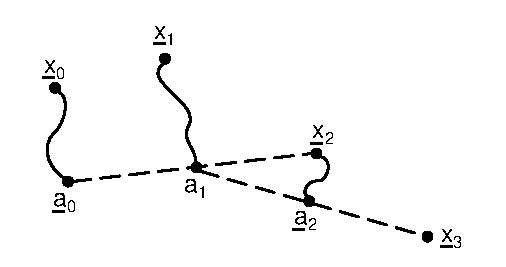
\epsfig{file=mi13.eps}}\end{center}
 
\begin{center}
Fig. 13
\end{center}
\end{figure}
 a `long' random step is taken to the
point ${\underline{x}}_1$, and another rough local minimization is performed to reach the
point ${\underline{a}}_1$(see figure above). Then the so-called `precipitous step' is
taken along a line from ${\underline{a}}_0$ to ${\underline{a}}_1$, some distance past
 ${\underline{a}}_1$ to ${\underline{x}}_2$.
Then from ${\underline{x}}_2$ another rough local
minimization is performed, yielding ${\underline{a}}_2$, and another
precipitous step is taken from ${\underline{a}}_1$ past ${\underline{a}}_2$ to ${\underline{x}}_3$ 
and the search continues in this way.
 
 
      The choice of the `precipitous step' length is important in determining whether the method
will `roll over small ridges, but skirt a high mountain', as its authors say it should. But no
precise way is given, except that `the choice of the length of the precipitous step is carried
out experimentally (by trials) and it constitutes an important
charactistic of the function'.
 
     Moreover, there is no stopping rule, since the method is essentially
searching rather than converging.  In practice one usually stops after
a given length of computer time, but one would also stop if the program
went around in circles repeating itself (which is very possible but not
so easy to detect) or if a predetermined `acceptably small' function
value was attained.  This problem of stopping seems to be common to all
non-local minimization methods.
 
\section{The Goldstein-Price method}
 
     Goldstein and Price \cite{Gold1} have proposed an elegant yet simple method
for seeking other local minima after one local minimum has been found
It is based on a consideration of the analytic (Taylor series) properties
of the function.  Let us assume that the function can be represented as
a Taylor series about a local minimum ${\underline{x}}_1$, where the first derivatives
vanish:
 
$$F({\underline{x}})~=~F({\underline{x}})_1~+~{1\over
2}~({\underline{x}}~-~{\underline{x}}_1)
^T\UTG({\underline{x}}-{\underline{x}}_1)~+~h.t.~.$$
 
Now the higher terms (h.t.), involving third and higher derivatives, are
important since these are the terms that will give rise to other local
minima.  In fact, we seek a way of transforming the function so that only
the higher terms remain.  Such a transformed function is $F_1$ such that:
$$F_1({\underline{x}}_1,{\underline{x}})~=~{2(F({\underline{x}})~-~F({\underline{x}}_1))\over
({\underline{x}}-{\underline{x}}_1)^T\UTG({\underline{x}}-{\underline{x}}_1)}~=~1~+~h.t.~.$$
 By means of this
transformation, we have `removed' the minimum at ${\underline{x}}_1$, and 
the way is cleared to search for other
minima generated by the higher terms of the expansion about ${\underline{x}}_1$.
  The method therefore consists of
seeking a local minimum of the function $F_1$  (It is required to know the
second derivative matrix $\UTG$ at the local minimum ${\underline{x}}_1$.)  Since the
quadratic form $({\underline{x}} - {\underline{x}}_1)^T \UTG({\underline{x}} -
{\underline{x}}_1)$
 is always positive for positive-definite $\UTG$, th
efunction $F_1$ will become negative as soon as an improvement on ${\underline{x}}_1$ is
found.  Then starting from this improved point, the original function $F$
can be minimized locally to yield a new, improved local minimum of $F$.
 
     If the minimum value found for $F_1$ is positive, 
then it may correspond to a new local minimum
of $F$, but not an improvement over ${\underline{x}}_1$.
 
In this case the procedure may be continued from this new point, forming
a new function $F_2$, related to $F_1$ just as $F_1$ was related to $F$. As usual,
no stopping rule is given by the theory.
 
     The method seems to work in practice, although experience with it
is limited and no conditions are known under which it is guaranteed to
work.  It is appealing for reasons of its elegance and simplicity, and
could prove to be an important tool in global minimization.
\newpage
\chapter*{Appendix: Some sample Problems for Minimization Routines}
     We assemble here a collection of test problems  found to be
useful in verifying and comparing different minimization routines.
Many of these are standard functions upon which it has become
conventional to try all new methods, quoting the performance in the
publication of the algorithm.
 
 
\section{Rosenbrock's curved valley}
 
                 $$ F(x,y)~=~100(y~-~x^2)^2~+~(1~-~x)^2$$
\noindent 
start point:{\phantom{xxxxxxxxxxxxxxxxxx}}$ F(-1.2,1.0)~=~24.20$
\vskip2mm
\noindent
minimum:{\phantom{xxxxxxxxxxxxxxxxxxx}}$ F(1.0,1.0)~=~0~.$
\vskip2mm
 
     This narrow, parabolic valley is probably the best known of all test
cases.  The floor of the valley follows approximately the parabola
$y = x^2$ + 1/200, indicated by the dashed line in fig. 14.  In the
cross-hatched area above the dashed line, the covariance matrix is not
positive-definite.  On the dashed line it is singular.  Stepping methods
tend to perform at least as well as gradient methods for this function.\\ \noindent
 [Reference:  Comput. J. {\bf 3}, 175 (1960).]
\begin{figure}[t]
\begin{center}\mbox{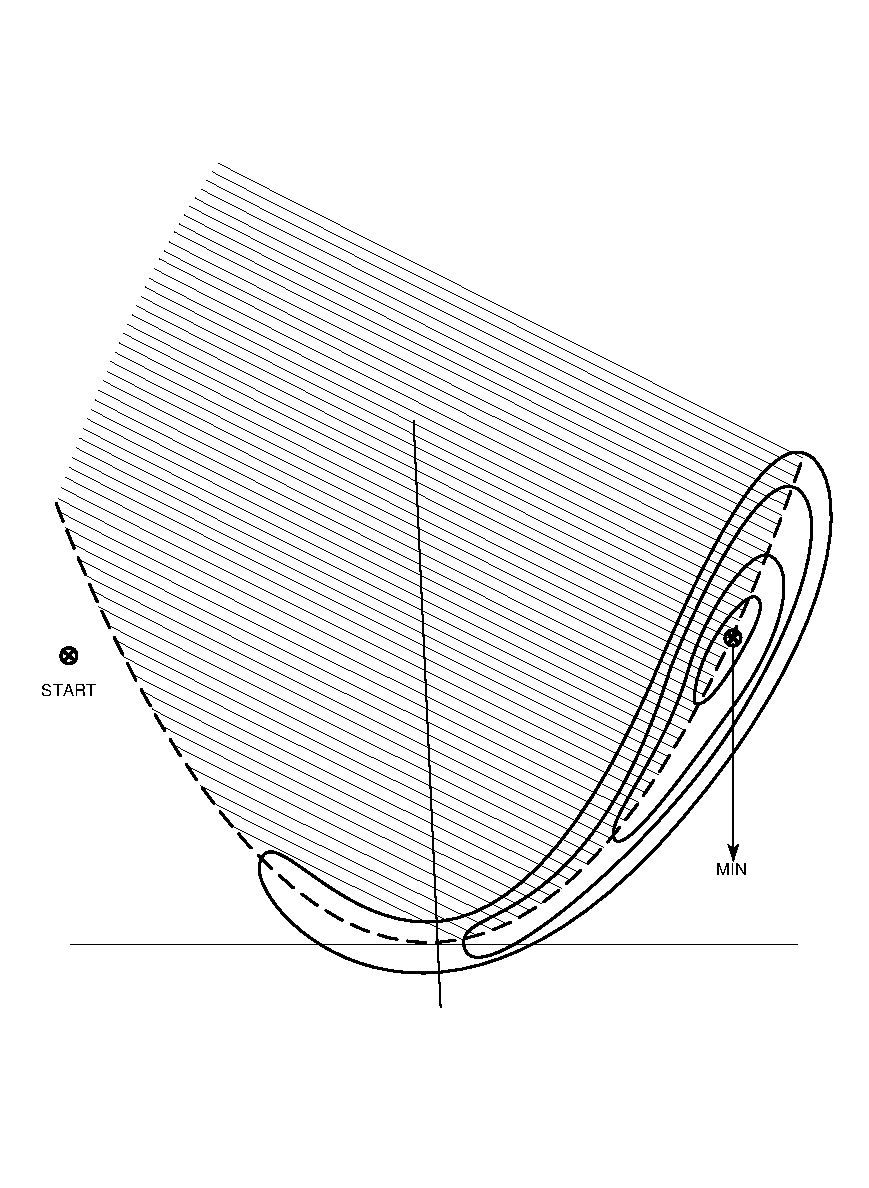
\epsfig{file=mi14.eps,width=10cm}}\\
Fig. 14
\end{center}
\end{figure}
 
 
\section{Wood's function of four parameters}
 
 
\begin{eqnarray}
  F(w,x,y,z)& =& 100(x~-~w^{2})^{2}~+~(w~-~1)^{2}~+~90(z~-~y^{2})^{2}\nonumber\\
              && +~(1~-~y)^{2}~+~10.1[(x~-~1)^{2}~+~(z~-~1)^{2}]~+~19.8(x~-~1)(z~-~1)\nonumber 
\end{eqnarray}
\noindent 
start point:{\phantom{xxxxxxxxxxxxxxxxxx}}$F(-3,-1,-3,-1)~=~19192$
\vskip2mm
\noindent
minimum:{\phantom{xxxxxxxxxxxxxxxxxxx}}$F(1,1,1,1)~=~0~.$
\vskip2mm 
     This is a fourth-degree polynomial which is reasonably well-behaved
near the minimum, but in order to get there one must cross a rather flat,
four-dimensional `plateau' which often causes minimization algorithm to
get `stuck' far from the minimum.  As such it is a particularly good
test of convergence criteria and simulates quite well a feature of many
physical problems in many variables where no good starting
approximation is known.\\ \noindent
[Reference:  Unpublished.  See IBM Technical Report No. 320--2949.]
 
 
\section{Powell's quartic function}
 
 
     $$F(w,x,y,z)~=~(w~+~10x)^2~+~5(y~-~Z)^2~+~(x~-~2y)^4~+~10(w~-~z)^4$$
\noindent 
start point:{\phantom{xxxxxxxxxxxxxxxxxx}}$F(3,-1,0,1)~=~215$
\vskip2mm
\noindent
minimum:{\phantom{xxxxxxxxxxxxxxxxxxx}}$ F(0,0,0,0)~=~0$ .
 \vskip2mm
     This function is difficult because its matrix of second derivatives
becomes singular at the minimum.  Near the minimum the function is given
by $(w~+~10x)^2~+~5(y~-~5)^2$ which does not determine the minimum uniquely.\\ \noindent
 [Reference:  Comput. J. {\bf 5}, 147 (1962).]
 
\section{Fletcher and Powell's helical valley}
 
 
$$F(x,y,z)~=~100\{[z~-~10\Psi(x,y)]^2~+~(\sqrt{x^2~+~y^2}~-~1)^2\}~+~z^2$$
\vskip2mm
\noindent
where 
\begin{tabular}{llll}             
$ 2\pi\Psi(x,y)$ &=& arctan $(y/x)$ &for $x > $0\\
                       &= &$\pi$ + arctan $(y/x)$& for $x < 0$
\end{tabular}
\vskip2mm
\noindent 
start point:{\phantom{xxxxxxxxxxxxxxxxxx}}$F(-1,0,0)~=~2500$
\vskip2mm
\noindent
minimum:{\phantom{xxxxxxxxxxxxxxxxxxx}}$F(1,0,0)~=~0~.$
\vskip2mm 
$F$ is defined only for $-0.25 < \Psi < 0.75$.
 
     This is a curved valley problem, similar to Rosenbrock's, but in
three dimensions.\\ \noindent
[Reference:  Comput. J. {\bf 6}, 163 (1963).]
 
 
\section{Goldstein and Price function with four minima}
 
 \begin{eqnarray}
     F(x,y)&=&(1~+~(x~+~y~+~1)^2 * (19-14x~+~3x^2~-~14y~+~6xy~+~3y^2))\nonumber\\
             &&*~(30~+~(2x~-~3y)^2 * (18-32x~+~12x^2~+~48y~-~36xy~+~27y^2))\nonumber
\end{eqnarray}
\vskip2mm
\noindent
local minima:{\phantom{xxxxxxxxxxxxxxxxxx}}$F$ (1.2, 0.8)~~~~\,= 840\\
{\phantom{xxxxxxxxxxxxxxxxxxxxxxxxxxxxx}}$F$ (1.8,0.2)~~~~~~= 84\\
{\phantom{xxxxxxxxxxxxxxxxxxxxxxxxxxxxx}}$F$ $(-0.6,-0.4)$~= 30\\
global minimum: {\phantom{xxxxxxxxxxxxxx}}$F$ $(0,-1.0)$~~~~~~= 3~.
 
\vskip2mm
 
     This is an eighth-order polynomial in two variables which is well
behaved near each minimum, but has four local minima and is of course
non-positive-definite in many regions.  The saddle point between the two
lowest minima occurs at $F(-0.4,-0.6)$ = 35, making this an interesting
start point.\\ \noindent
 [Reference:  Math. Comp. {\bf 25}, 571 (1971).]
 
 
 \section{Goldstein and Price function with many minima}
 
 
$$F(x,y)~=~\exp \left\{{1\over 2}~(x^2~+~y^2~-~25)^2\right\}~+~\sin^4 (4x~-~3y)~+~{1\over 2}~
(2x~+~y~-~10)^2$$  
 \noindent
 global minimum:{\phantom{xxxxxxxxxxxxxxxxxx}}$F  (3,4)~=~1~.$\vskip2mm \noindent
      This function has `many' local minima.\\ \noindent
[Reference:  Math. Comp. {\bf 25}, 571 (1971).]
 
 
\section{Quadratic function in four parameters}
 
 
 
        $$F(x,y,z,w)~=~{1\over 70}~(21x^2~+~20y^2~+~19z^2~-~14xz~-~20yz)~+~w^2$$
\noindent 
minimum:{\phantom{xxxxxxxxxxxxxxxxxxx}}$ F(0,0,0,0)~=~0$                          
\vskip1cm
\noindent
 covariance~matrix:
 
\hskip10cm
\vskip-2.2cm
\begin{eqnarray*}
\left(\begin{array}{cccc}4&1&2&0\\
1&5&3&0\\
2&3&6&0\\
0&0&0&1
\end{array}
\right)
\end{eqnarray*}
 
     Except for the reasonably strong parameter correlations, this function
poses no special problem to any minimization routine.  But the
author has found it useful in debugging programs based on quadratically
convergent methods, since these programs should minimize the function
exactly in one iteration.  It is also used to check the calculation of
the covariance matrix.
 
     A variation consists of adding $|x|^3~-~1$ whenever $|x| >$ 1, and
similarly with the other variables.  This introduces in a reasonably
smooth way terms which alter the quadratic behaviour far from the
minimum
while leaving it unchanged inside the unit cube, thus providing a test
for those methods which are supposed to converge to the correct
covariance matrix by updating.
 
\section{Chebyquad}
 
 
$$F(\vec{x})~=~\sum^{n}_{i=1}~\left\{\int^1_0~T_i(x^{\prime})~dx^{\prime}~-~{1\over
n}~\sum^{n}_{j=1}~T_i (x_j)\right\}^{2}$$
where $T_i(x)$ are shifted Chebyshev polynomials of degree i;\vskip2mm
\noindent 
start point:{\phantom{xxxxxxxxxxxxxxxxxx}}$x_j~=~j/(n + 1)~.$
\vskip2mm
     This function is designed to have a variable and possibly large
number of parameters, and to resemble functions encountered in actual
practice rather than being contrived to be especially difficult.  Each
term of $F$ represents the squared difference between the true integral
of a polynomial of degree $i$ and the integral estimated by Chebyshev
(equal-weight) quadrature on $n$ points:
 $$\int^{1}_{0}~P(x)~dx~\approx~{1\over n}~\sum^{n}_{j=1}~P(x_j)~.$$
 
The starting values correspond to equally spaced points $x_j$ which is not
too far away from the solution.  Fletcher gives a complete Algol-coded,
procedure for this function in the reference quoted below.\\ \noindent
 [Reference:  Comput. J. {\bf 8}, 33 (1965).]
 
\section{Trigonometric functions of Fletcher and Powell}
$$F(\vec{x})~=~\sum^{n}_{i=1}~\left\{E_i~-~\sum^{n}_{j=1}~(A_{ij}~
\sin~x_j~+~B_{ij}~\cos~x_j)\right\}^{2}~,$$
where
 
 $$E_i~=~\sum^{n}_{j=1}~(A_{ij}~
\sin~x_{0j}~+~B_{ij}~\cos~x_{0j})~.$$
 
$B_{ij} $ and $A_{ij}$ are random matrices composed of integers between -100 and
100;  for $j$ = 1, ..., $n$:  $x_{0j}$ are any random numbers, $-\pi < x_{0j} < \pi;$\vskip2mm
\noindent 
start point:{\phantom{xxxxxxxxxxxxxxxxxx}}$x_j~=~x_{0j}~+~0.1\delta_j, -\pi < \delta j < \pi$
\vskip2mm
\noindent
minimum:{\phantom{xxxxxxxxxxxxxxxxxxx}}$F(\vec{x}~=~\vec{x}_0)~=~0~. $
\vskip2mm 
     This is a set of functions of any number of variables $n$, where the
minimum is always known in advance, but where the problem can be changed
by choosing different (random) values of the constants $A_{ij}, B_{ij}$, and $x_{0j}$. 
The difficulty can be varied by choosing larger starting deviations  $\delta_j$. 
In practice, most methods find the `right' minimum, corresponding to
$\vec{x}~=~\vec{x}_0$, but there are usually many subsidiary minima.\\ \noindent
 [Reference:  Comput. J. {\bf 6} 163 (1963).]

%%\part{The Interpretation of Errors}
%	$Id: minerror.tex,v 1.4 1998/08/19 11:48:33 goossens Exp goossens $	
%%%%%%%%%%%%%%%%%%%%%%%%%%%%%%%%%%%%%%%%%%%%%%%%%%%%%%%%%%%%%%%%%%%
%                                                                 %
%   MINUIT User Guide -- LaTeX Source                             %
%                                                                 %
%   Part 2: Chapter on error interpretation                       %
%                                                                 %
%   The following external EPS files are referenced:              %
%      minoserr.eps,minosco1.eps,minosco2.eps,minosco3.eps        %
%                                                                 %
%   Editor: Michel Goossens / CN-AS                               %
%   Last Mod.: 26 Jan. 1993 18:00 mg                              %
%                                                                 %
%%%%%%%%%%%%%%%%%%%%%%%%%%%%%%%%%%%%%%%%%%%%%%%%%%%%%%%%%%%%%%%%%%%
 
\chapter{Interpretation of the errors on Minuit parameters}
 
It often happens that the solution of a minimization problem using
Minuit is itself straightforward, but the calculation or
interpretation of the resulting parameter uncertainties is
considerably more complicated. The purpose of this chapter is to
clarify the most commonly encountered difficulties in parameter error
determination. These difficulties may arise in connection with any
fitting program, are discussed here with Minuit terminology.
 
The most common causes of misinterpretation may be grouped into 
three categories:
 
\begin{OL}
\item Proper normalization of the user-supplied chi-square or
  likelihood function, and appropriate \Cind[SET ERRordef]{ERROR DEF}.
\item Non-linearities in the problem formulation, leading to different
  errors being calculated by different techniques, such as
  \Cind[MIGrad]{MIGRAD}, \Cind[HESse]{HESSE} and \Cind[MINos]{MINOS}.
\item Multiparameter error definition and interpretation.
\end{OL}
 
All these topics are discussed in some detail in Eadie et
al.\cite{bib-EADIE}, which may be consulted for further details.
 
\section{Function normalization and ERROR DEF}
 
In order to provide for full generality in the user-defined function
value, the user is allowed to define a normalization factor known
internally as \texttt{UP} and defined by the Minuit user on an
\Cind[SET ERRordef]{ERROR DEF} command card.  The default value is
one. The Minuit error on a parameter is defined as the change of
parameter which would produce a change of the function value equal to
\texttt{UP}.  This is the most general way to define the error,
although in statistics it is more usual to define it in terms of the
second derivative of the $\chi^2$ function -- with respect to the
parameter in question. In the simplest linear case (when the function
is exactly parabolic at the minimum), the value \texttt{UP=1.0}
corresponds to defining the error as the inverse of the second
derivative at the minimum. The fact that Minuit defines the error in
terms of a function change does not mean that it always calculates
such a function change. Indeed it sometimes (\Cind[HESse]{HESSE})
calculates the second derivative matrix and inverts it, assuming a
parabolic behaviour. This distinction is discussed in section
\ref{sec:errornonlin}.
 
The purpose of defining errors by function changes is threefold: 

\begin{OL}
\item to preserve its meaning in the non-parabolic case (see section
  \ref{sec:errornonlin});
\item to allow generality when the user-defined function is not a chi-
  square or likelihood, but has some other origin;
\item to allow calculation not only of ``one-standard deviation''
  errors, but also two or more standard deviations, or more general
  'confidence regions', especially in the multiparameter case (see
  section \ref{sec:errormultipar}).
\end{OL}
 
\subsection{Chi-square normalization}
 
If the user's function value $F$ is supposed to be a chisquare, it must 
of course be properly normalized. That is, the ``weights'' must in fact 
correspond to the one-standard-deviation errors on the observations. 
The most general expression for the chi-square $\chi$ is of 
the form (see \cite{bib-EADIE}, p.163):
 
\[ \chi^2 = \sum_{i,j} (x_i - y_i(a)) V_{ij} (x_j - y_j(a)) \]
 
where $x$ is the vector of observations, $y(a)$ is the vector of fitted 
values (or theoretical expressions for them) containing the variable 
fit parameters $a$, and $V$ is the inverse of the error matrix of the 
\index{covariance matrix}
observations $x$, also known as the covariance matrix of the 
observations.
 
Fortunately, in most real cases the observations $x$ are statistically 
independent of each other (e.g., the contents of the bins of a 
histogram, or measurements of points on a trajectory), so the 
matrix $V$ is diagonal only. The expression for $\chi^2$ then simplifies to 
the more familiar form:
 
\[ \chi^2 = \sum_{i} \frac{(x_i - y_i(a))^2}{e_i^2} \]
 
where $e^2$ is the inverse of the diagonal element of $V$, the square of 
the error on the corresponding observation $x$. In the case where the $x$
are integer numbers of events in an unweighted histogram, for 
example, the $e^2$ are just equal to the x (or to the y, see \cite{bib-EADIE},
pp.170-171).
 
The minimization of $\chi^2$ above is sometimes called {\bf weighted least 
\index{weighted least squares}%
\index{least squares!weighted}%
squares} in which case the inverse quantities $1/e^2$ are called the weights. 
Clearly this is simply a different word for the same thing, 
but in practice the use of these words sometimes means that the 
interpretation of $e^2$ as variances or squared errors is not 
straightforward. The word weight often implies that only the 
relative weights are known (``point two is twice as important as 
point one'') in which case there is apparently an unknown overall 
normalization factor. Unfortunately the parameter errors coming out 
of such a fit will be proportional to this factor, and the user must be 
aware of this in the formulation of his problem.
                                                                                               
The $e^2$ may also be functions of the fit parameters $a$ (see \cite{bib-EADIE},
pp.170-171). Normally this results in somewhat slower convergence 
of the fit since it usually increases the nonlinearity of the fit. (In 
the simplest case it turns a linear problem into a non-linear one.) 
However, the effect on the fitted parameter values and errors should 
be small.
 
If the user's chi-square function is correctly normalized, he should 
\index{standard deviation}
use \texttt{UP=1.0} (the default value) to get the usual 
one standard-deviation errors for the parameters one by one. 
To get two-standard-dev.eviation
errors, use \Cind[SET ERRordef]{ERROR DEF 4.0}, etc., 
since the chisquare dependance on 
parameters is quadratic. For more general confidence regions 
involving more than one parameter, see section \ref{sec:errornonlin}.
 
\subsection{Likelihood normalization}
\index{likelyhood}

If the user function is a negative log-likelihood function, it must 
again be correctly normalized, but the reasons and ensuing problems 
in this case are quite different from the chisquare case. The 
likelihood function takes the form (see \cite{bib-EADIE}, p. 155):
 
\[ F = - \sum_{i} \ln f(x_i,a) \]
 
where each $x$ represents in general a vector of observations, the $a$ 
are the free parameters of the fit, and the function $f$ represents the 
hypothesis to be fitted. This function $f$ must be normalized:
 
\[ \int f(x_i,a) \mathrm{d}x_1 \mathrm{d}x_2 \ldots 
                 \mathrm{d}x_n = \mathrm{constant} \]
 
that is, the integral of $f$ over all observation space $x$ must be 
independent of the fit parameters $a$.
 
The consequence of not normalizing $f$ properly is usually that the fit 
simply will not converge, some parameters running away to infinity. 
Strangely enough, the value of the normalization constant does not 
affect the fitted parameter values or errors, as can be seen by the 
fact that the logarithm makes a multiplicative constant into an 
additive one, which simply shifts the whole log-likelihood curve and 
affects its value, but not the fitted parameter values or errors. In 
fact, the actual value of the likelihood at the minimum is quite 
meaningless (unlike the chi-square value) and even depends on the 
units in which the observation space $x$ is expressed. The meaningful 
quantity is the difference in log-likelihood between two points in 
parameter-space, which is dimensionless.
 
For likelihood fits, the value \texttt{UP=0.5} corresponds to 
one-standard-deviation errors. 
Or, alternatively, $F$ may be defined as $-2\log(\mathrm{likelihood})$, 
in which case differences in $F$ have the same meaning as for chi-square 
and \texttt{UP=1.0} is appropriate. The two different ways of introducing the 
factor of 2 are quite equivalent in Minuit, and although most people 
seem to use \texttt{UP=0.5}, it is perhaps more logical to put the 
factor 2 directly into \Rind{FCN}.
 
\section{Non-linearities: MIGRAD versus HESSE versus MINOS}
\label{sec:errornonlin}

In the theory of statistics, one can show that in the asymptotic
limit, any of several methods of determining parameter errors are
equivalent and will give the same result.  Let us for the moment call
these methods \Cind[MIGrad]{MIGRAD}, \Cind[HESse]{HESSE}, and
\Cind[MINos]{MINOS} (\Cind[SIMplex]{SIMPLEX} is a special case).  It
turns out that the conditlons under which these methods yield exactly
the same errors are either of the following:
 
\begin{OL}
\item The model to be fitted ($y$ or $f$) is exactly a linear function of the 
      fit parameters $a$, or
\item The amount of observed data is infinite.
\end{OL}
 
It may happen that (1) is  satisfied, in whlch case you don't really 
need Minuit, a smaller, simpler, and faster program would do, since 
a linear problem can be solved directly without iterations (see \cite{bib-EADIE},
p. 163-165), for example with CERN library program \texttt{LSQQR}. 
Nevertheless, it may be convenient to use Minuit slnce non-linear 
terms can then be added later if desired, without major changes to 
the method. Condition (2) is of course never satisfied, although in 
practice it often happens that there is enough data to make the 
problem ``almost linear'', that is there is so much data that the 
range of parameters allowed by the data becomes very small, and 
any physical function behaves linearly over a small enough region.
 
The following sections explain the dirrerences between the various 
parameter errors given by Minuit.
 
\subsection{Errors printed by Minuit}
 
The errors printed by Minuit at any given stage represent the best 
symmetric error estimates available at that stage, which may not 
be very good. For example, at the first entry to \Rind{FCN}, the user's step 
slzes are given, and these may bear no resemblance at all to proper 
parameter errors, although they are supposed to be order-of-magnltude estimates. 
After crude minimizers like \Cind[SEEk]{SEEK} or \Cind[SIMplex]{SIMPLEX}, 
a revised error estimate may be given, but this too is only meant to
be an order-or-magnitude estimate, and must certainly not be 
taken seriously as a physical result. Such numbers are mainly for 
the internal use of Minuit, which must after all assume a step size 
for future minimizations and derivative calculations, and uses these 
``errors'' as a first guess to be modified on the basis of experience.
 
\subsection{Errors after MIGRAD (or MINIMIZE)}
 
The minimizing technique currently implemented in \Cind[MIGrad]{MIGRAD} is a 
stable variation (the ``switching'' method) of the 
Davidon-Fletcher-Powell variable-metric algorithm.
This algorithm converges to the correct error matrix as it converges 
to the function minimum. 

This algorithm requires at each step a ``working approximation'' of the
error matrix, and a rather good approximation to the gradient vector at
the current best point. 
The starting approximation to the error matrix may be obtained in different
ways, depending on the status of the error matrix before MIGRAD is called
as well as the value of STRATEGY.  Usually it is found to be advantageous 
to evaluate the error matrix rather carefully at the start point in order
to avoid premature convergence, but in principle even the unit matrix
can be used as a starting approximation.  
Usually the Minuit default is to start by calculating the full error matrix by
calculating all the second derivatives and inverting the matrix.
If the user wants to make sure this is done, he can call HESSE before MIGRAD.

If a unit matrix is taken to start,
then the first step will be in a {\em steepest descent} direction, which is
not bad, but the estimate of EDM, needed to judge convergence, will be poor.
At each successive step, the information gathered from the change of gradient
is used to improve the approximation to the error matrix, without the need
to calculate any second derivatives or invert any matrices.
The algorithm used for this {\em updating} is supposed to be the best known,
but if there are a lot of highly correlated parameters, it may take many steps
before the off-diagonal elements of the error matrix approach the correct values.

In practice, \Cind[MIGrad]{MIGRAD} usually yields good estimates of the 
error matrix, but it is not absolutely reliable for two reasons:
 
\begin{OL}
\item Convergence to the minimum may occur ``too fast'' for \Cind[MIGrad]{MIGRAD} to 
      have a good estimate of the error matrix. In the most flagrant of 
      such cases, \Cind[MIGrad]{MIGRAD} realizes this and automatically introduces an 
      additional call to \Cind[HESse]{HESSE} (described below), informing the user that 
      the covariance matrix is being recalculated. Since, for $n$ variable 
      parameters, there are $n(n+1)/2$ elements in the error matrix, the 
      number of \Rind{FCN} calls from \Cind[MIGrad]{MIGRAD} must be large compared with 
      $n^2$ in order for the \Cind[MIGrad]{MIGRAD} error matrix calculation to be 
      reliable.
\item \Cind[MIGrad]{MIGRAD} gathers information about the error matrix as it 
      proceeds, based on function values calculated away from the 
      minimum and assuming that the error matrix is nearly constant as a 
      function of the parameters, as it would be if the problem were 
      nearly linear. If the problem is highly non-linear, the error matrix 
      will depend strongly on the parameters, \Cind[MIGrad]{MIGRAD} will converge more 
      slowly, and the resulting error matrix will at best represent some 
      average over the last part of the trajectory in parameter-space 
      traversed by \Cind[MIGrad]{MIGRAD}.
\end{OL}
 
If \Cind[MIGrad]{MIGRAD} errors are wrong because of (1),
\Cind[HESse]{HESSE} should be commanded after \Cind[MIGrad]{MIGRAD} 
and will give the correct errors. If \Cind[MIGrad]{MIGRAD} 
errors are wrong because of (2), \Cind[HESse]{HESSE} will help, but only in an 
academic sense, since in this case the error matrix is not the whole 
story and for proper error calculation \Cind[MINos]{MINOS} must be used.
 
As a general rule, anyone seriously interested in the parameter 
errors should always put at least a \Cind[HESse]{HESSE} command after each 
\Cind[MIGrad]{MIGRAD} (or \Cind[MINImize]{MINIMIZE}) command.
 
\subsection{Errors after HESSE}
 
\Cind[HESse]{HESSE} simply calculates the full second-derivative matrix by finite 
differences and inverts it. It therefore calculates the error matrix 
at the point where it happens to be when it is called. If the error 
matrix is not positive-definite, diagnostics are printed, and an 
\index{error matrix}
attempt is made to form a positive-definite approximation. The 
error matrix must be positive-definite at the solution (minimum) 
for any real physical problem. It may well not be positive away from 
the minimum, but most algorithms including the \Cind[MIGrad]{MIGRAD} algorithm 
require a positive-definite ``working matrix''.
 
The error matrix produced by \Cind[HESse]{HESSE} is used to calculate what Minuit 
prints as the parameter errors, which therefore contain the effects 
due to parameter correlations. The extent of the two-by-two 
correlations can be seen from the correlation coefficients printed by 
Minuit, and the global correlations (see \cite{bib-EADIE}, p. 23) are also 
printed. All of these correlation coefficients must be less than one 
in absolute value. If any of them are very close to one or minus one, 
this indicates an illposed problem with more free parameters than 
can be determined by the model and the data.
 
\subsection{Errors by MINOS}
 
\Cind[MINos]{MINOS} is designed to calculate the correct errors in all cases, 
especially when there are non-linearities as described above. The 
theory behind the method is described in \cite{bib-EADIE}, pp. 204-205 
(where ``non-parabolic likelihood'' should of course read 
``non-parabolic log-likelihood'', 
which is equivalent to ``nonparabolic chi-square'').
 
\Cind[MINos]{MINOS} actually follows the function out from the minimum to find 
where it crosses the function value (minimum + \texttt{UP}), instead of using 
the curvature at the minimum and assuming a parabolic shape. This 
method not only yields errors which may be different from those of 
\Cind[HESse]{HESSE}, but in general also different positive and negative errors 
(asymmetric error interval). Indeed the most frequent result for 
most physical problems is that the (symmetric) \Cind[HESse]{HESSE} error lies 
between the positive and negative errors of \Cind[MINos]{MINOS}. The difference 
between these three numbers is one measure of the non-linearity of 
the problem (or rather of its formulation).
 
In practice, \Cind[MINos]{MINOS} errors usually turn out to be close to, or 
somewhat larger than errors derived from the error matrix, although 
in cases of very bad behaviour (very little data or ill-posed model) 
anything can happen. In particular, it is often not
true in \Cind[MINos]{MINOS} that two-standard-deviation errors 
(\texttt{UP=4}) and three-standard-deviation  errors (\texttt{UP=9}) 
are respectively two and three times as big as one-standard-deviation errors, 
as is true by definition for errors derived from the 
error matrix (\Cind[MIGrad]{MIGRAD} or \Cind[HESse]{HESSE}).

\section{Multiparameter errors}
\label{sec:errormultipar}
 
In addition to the difficulties described above, a special class of 
problems arise in interpreting errors when there is more than one 
free parameter. These problems are quite separate from those 
described above and are really much simpler in principle, although in 
practice confusion often arises.
 
\subsection{The Error Matrix}
\index{error matrix}
\index{covariance matrix}
 
The error matrix, also called the covariance matrix, is the inverse of 
the second derivative matrix of the (log-likelihood or chisquare) 
function with respect to its free parameters, usually assumed to be 
evaluated at the best parameter values (the function minimum). The 
diagonal elements of the error matrix are the squares of the 
\index{correlations}%
individual parameter errors, {\bf including the effects of correlations}
with the other parameters.
 
The inverse of the error matrix, the second derivative matrix, has as 
diagonal elements the second partial derivatives with respect to one 
parameter at a time. These diagonal elements are not therefore 
coupled to any other parameters, but when the matrix is inverted, 
the diagonal elements of the inverse contain contributions from all 
the elements of the second derivative matrix, which is ``where the 
correlations come from''.
 
Although a parameter may be either positively or negatively 
correlated with another, the effect of correlations is always to 
increase the errors on the other parameters in the sense that if a 
given free parameter suddenly became exactly known (fixed), that 
would always decrease (or at least not change) the errors on the 
other parameters. In order to see this effect quantitatively, the 
following procedure can be used to ``delete'' one parameter from the 
error matrix, including its effects on the other parameters:
 
\begin{OL}
\item Invert the error matrix, to yield the second-derivative matrix.
\item Remove the row and column of the inverse corresponding to the 
      given parameter.
\item Re-invert the resulting (smaller) matrix.
\end{OL}
 
This reduced error matrix will have its diagonal elements smaller or 
equal to the corresponding elements in the original error matrix, the 
difference representing the effect of knowing or not knowing the 
true value of the parameter that was removed at step two. This 
procedure is exactly that performed by Minuit when a \Cind{FIX} command 
is executed. Note that it is not reversible, since information has 
been lost in the deletion. 
The Minuit commands \Cind[REStore]{RESTORE} and 
\Cind[RELease]{RELEASE} therefore cause the error matrix to be considered lost and 
it must be recalculated entirely.
 
\subsection{MINOS with several free Parameters}

The \Cind[MINos]{MINOS} algorithm is described in some detail in part
1 of this manual.  Here we add some supplementary ``geometrical
interpretation'' for the multidimensional case.
 
Let us consider that there are just two free parameters, and draw 
the contour line connecting all points where the function takes on 
the value $F_{\mathrm{min}} + \mbox{\tt UP}$. 
(The \Cind[CONtour]{CONTOUR} command will do this for you from Minuit). 
For a linear problem, this contour line would be an 
exact ellipse, the shape and orientation of which are described in 
\cite{bib-EADIE}, p.196 (Fig. 9.4). 
For our problem let the contour be as in figure \ref{fig:MINoserror}.
If \Cind[MINos]{MINOS} is requested to find the errors in parameter 
one (the x-axis), it will find the extreme contour points A and B, 
whose x-coordinates, relative to the x-coordinate at the minimum 
(X), will be respectively the negative and positive \Cind[MINos]{MINOS} errors of 
parameter one.
 
\subsection{Probability content of confidence regions}
 
For an $n$-parameter problem \Cind[MINos]{MINOS} performs 
minimizations in $(n-1)$
dimensions in order to find the extreme points of the hypercontour 
of which a two-dimensional example is given in figure 
\ref{fig:MINoserror}, and in this 
way takes account of all the correlations with the other $n-1$
parameters. 
However, the errors which it calculates are still only 
single-parameter errors, in the sense that each parameter error is 
a statement only about the value of that parameter. 
This is 
represented geometrically by saying that the confidence region 
expressed by the \Cind[MINos]{MINOS} error in parameter one is the grey
area of figure \ref{fig:MINosconf1}, 
extending to infinity at both the top and bottom of the figure.
 
%begin{latexonly}
\begin{figure}[ht]
\begin{minipage}{.49\linewidth}
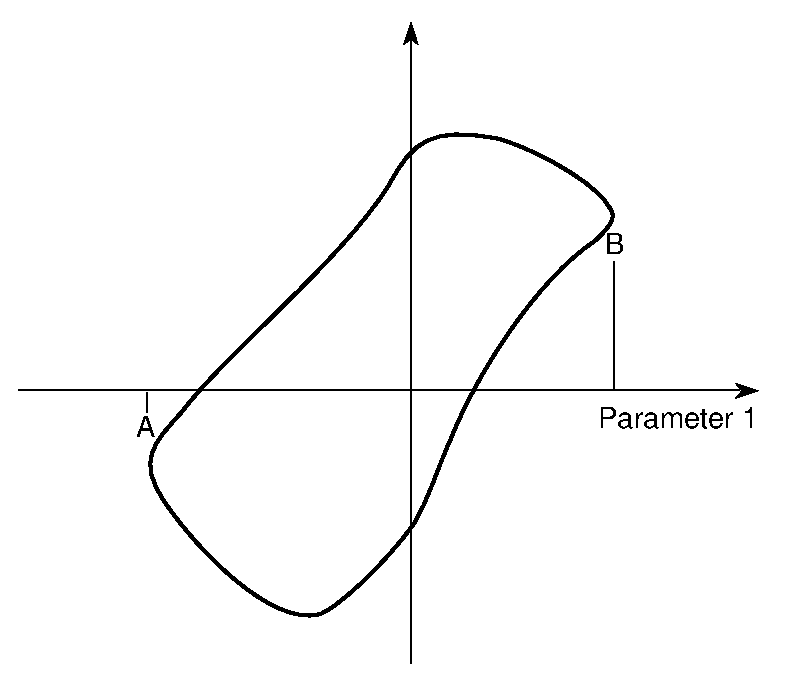
\includegraphics[width=\linewidth]{minoserr.eps}
\caption[MINOS errors for parameter 1]%
        {\Cind[MINos]{MINOS} errors for parameter 1}
\label{fig:MINoserror}
\end{minipage}\hfill
\begin{minipage}{.49\linewidth}
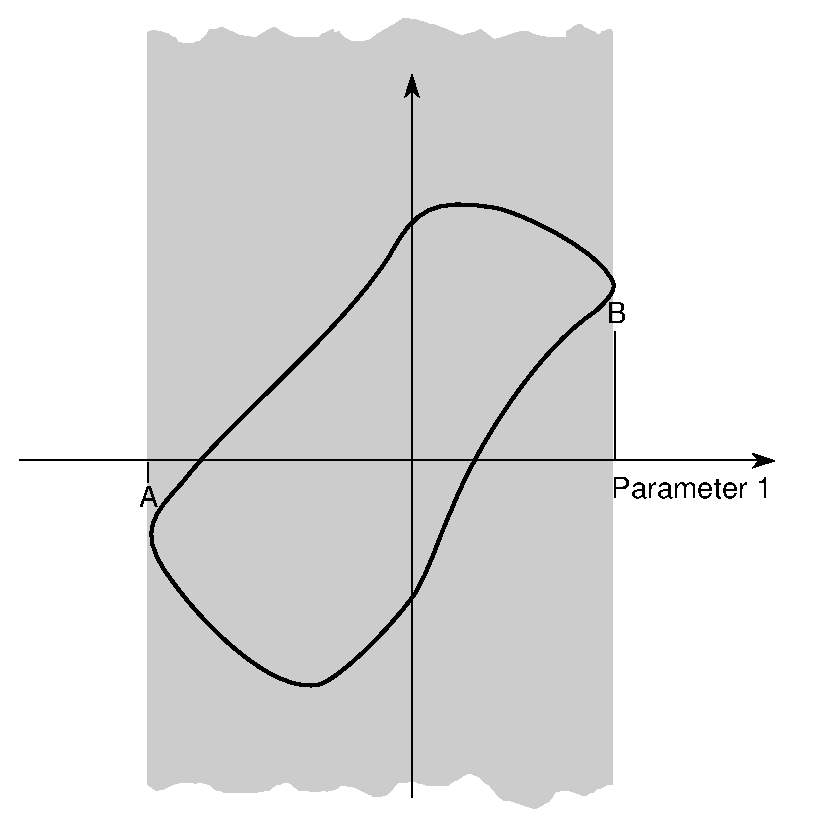
\includegraphics[width=\linewidth]{minosco1.eps}
\caption[MINOS error confidence region for parameter 1]%
        {\Cind[MINos]{MINOS} error confidence region for parameter 1}
\label{fig:MINosconf1}
\end{minipage}
\end{figure}
%end{latexonly}

\begin{htmlonly}
\begin{rawhtml}<P>\end{rawhtml}
\begin{figure}
\begin{makeimage}
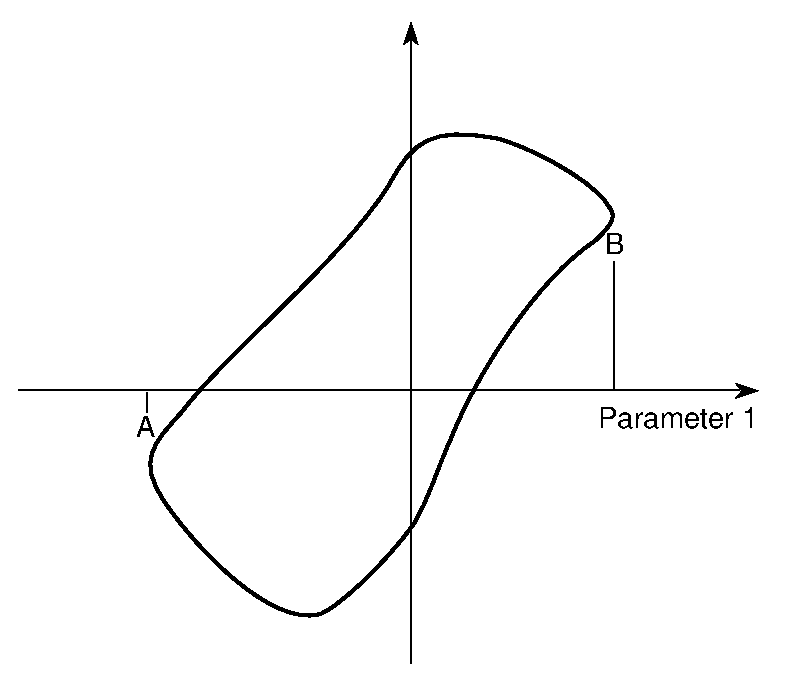
\includegraphics[width=\linewidth]{minoserr.eps}
\end{makeimage}
\caption{MINOS errors for parameter 1}
\label{fig:MINoserror}
\end{figure}

\begin{rawhtml}<P>\end{rawhtml}
\begin{figure}
\begin{makeimage}
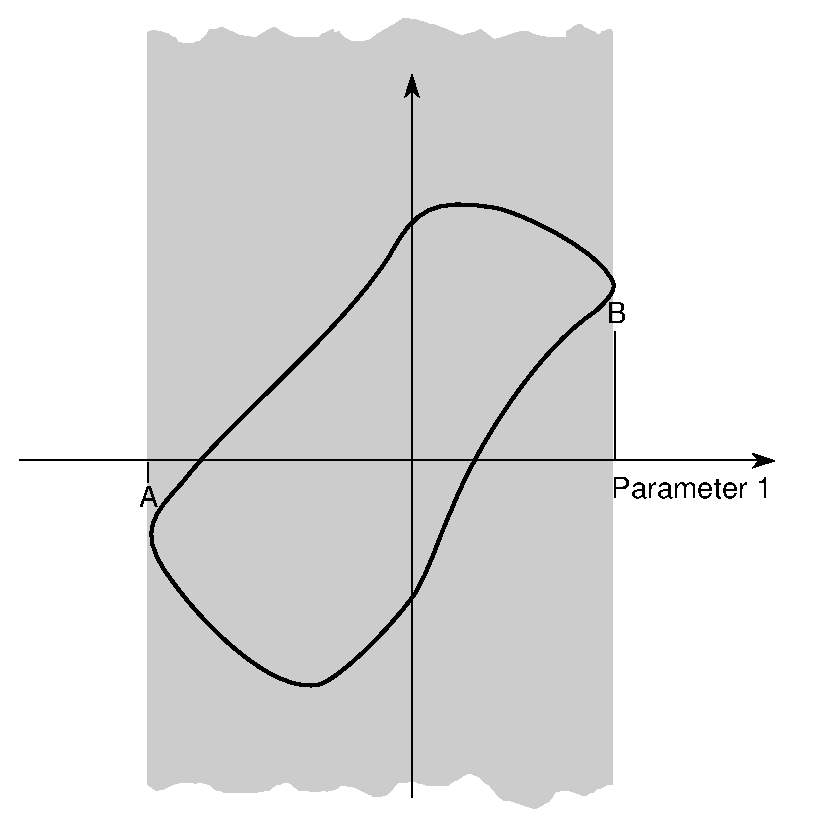
\includegraphics[width=\linewidth]{minosco1.eps}
\end{makeimage}
\caption{MINOS error confidence region for parameter 1}
\label{fig:MINosconf1}
\end{figure}
\begin{rawhtml}<P>\end{rawhtml}
\end{htmlonly}
 
If \texttt{UP} is set to the appropriate one-standard-deviation value, 
then the precise meaning of the confidence region of figure 
\ref{fig:MINosconf1} is:  ``The probability 
that the true value of parameter one lies between A and B is 68.3\%''
(the probability of a normally-distributed parameter lying within 
one std.-dev. of its mean). 
That is, the probability content of the 
grey area in figure \ref{fig:MINosconf1} is 68.3\%. 
No statement is made about 
the simultaneous values of the other parameter(s), since the grey
area covers all values of the other parameter(s).
 
If it is desired to make {\bf simultaneously} statements about the values 
of two or more parameters, the situation becomes considerably more 
complicated and the probabilities get much smaller. 
The first problem is 
that of choosing the shape of the confidence region, since it is no 
longer simply an interval on an axis, but a hypervolume. The easiest 
shape to express is the hyperrectangle given by: 

%begin{latexonly}
\begin{center}
\begin{tabular}{>{\tt}l}
A < param 1 < B \\
C < param 2 < D \\
E < param 3 < F , {\rm etc.}
\end{tabular}
\end{center}
%end{latexonly}
\begin{htmlonly}
\begin{alltt}
A < param 1 < B 
C < param 2 < D 
E < param 3 < F, \textrm{etc.}
\end{tabular}
\end{alltt}
\end{htmlonly}


This confidence region for our two-parameter example is the 
grey area in figure \ref{fig:MINosconf2}. 
However, there are two good reasons 
not to use such a shape:
 
\begin{enumerate}
\item Some regions inside the hyperrectangle (namely the corners) have 
      low likelihoods, lower than some regions just outside the rectangle, 
      so the hyperrectangle is not the optimal shape (does not contain the 
      most likely points).
\item One does not know an easy way to calculate the probability 
      content of these hyperrectangles (see~\cite{bib-EADIE}, p.196-197, 
      especially fig. 9.5a).
\end{enumerate} 

For these reasons one usually chooses regions delimited by contours 
of equal likelihood (hyperellipsoids in the linear case). For our 
two-parameter example, such a confidence region would be the grey
region in figure \ref{fig:MINosconf3}, and the corresponding probability 
statement is: ``The probability that parameter one and parameter two 
simultaneously take on values within the one-standard-deviation likelihood 
contour is 39.3\%''.
 
The probability content of confidence regions like those shaded in 
figure \ref{fig:MINosconf3} becomes very small as the number of parameters 
\texttt{NPAR} increases, for a given value of \texttt{UP}. 
Such probability contents are in 
fact the probabilities of exceeding the value \texttt{UP} for a chisquare 
function of \texttt{NPAR} degrees of freedom, and can therefore be read off 
from tables of chisquare. 
Table \ref{tab:MINosconf} gives the values of \texttt{UP} which 
yield hypercontours enclosing given probability contents for given 
number of parameters.

%begin{latexonly}
\begin{figure}[ht]
\begin{minipage}{.49\linewidth}
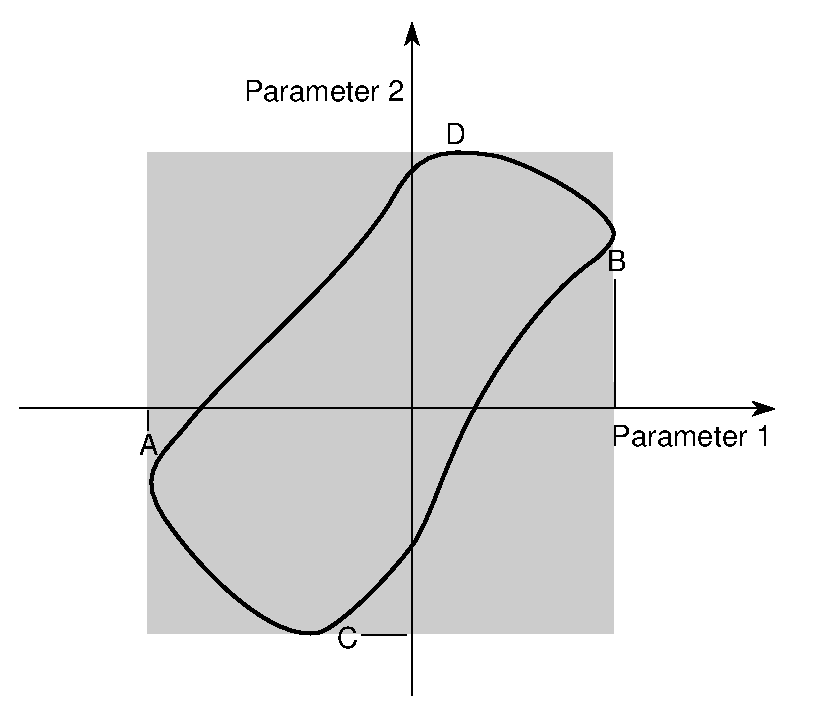
\includegraphics[width=\linewidth]{minosco2.eps}
\caption{Rectangular confidence region for parameters 1 and 2}
\label{fig:MINosconf2}
\end{minipage}\hfill
\begin{minipage}{.49\linewidth}
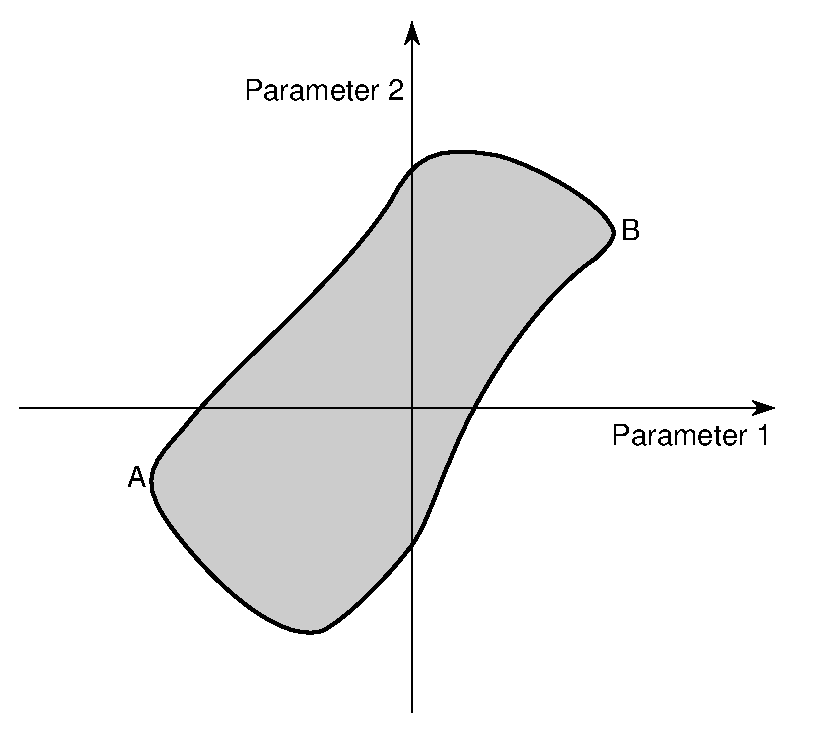
\includegraphics[width=\linewidth]{minosco3.eps}
\caption{Optimal confidence region for parameters 1 and 2}
\label{fig:MINosconf3}
\end{minipage}
\end{figure}
%end{latexonly}

\begin{htmlonly}
\begin{rawhtml}<P>\end{rawhtml}
\begin{figure}
\begin{makeimage}
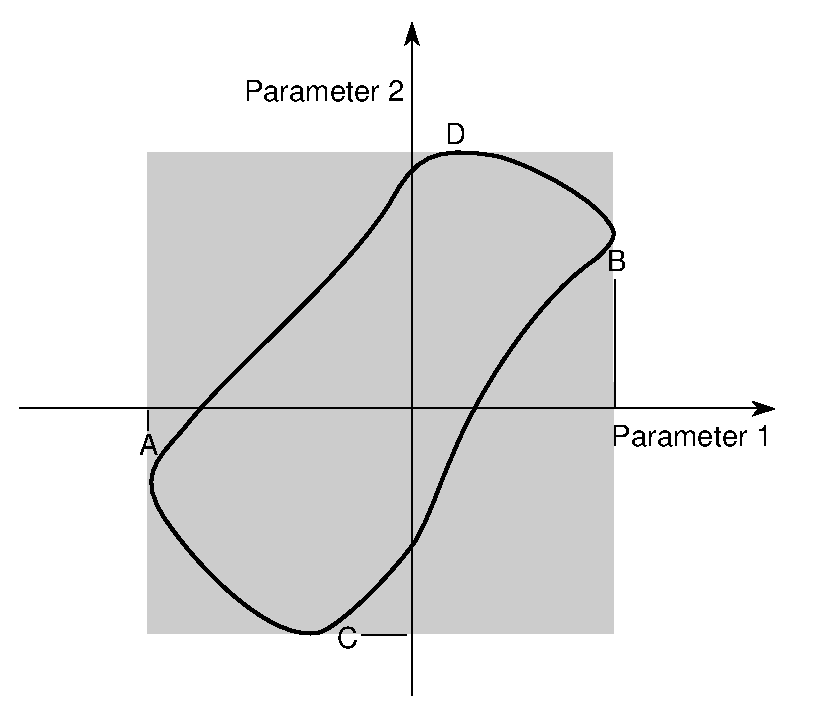
\includegraphics[width=\linewidth]{minosco2.eps}
\end{makeimage}
\caption{Rectangular confidence region for parameters 1 and 2}
\label{fig:MINosconf2}
\end{figure}

\begin{rawhtml}<P>\end{rawhtml}

\begin{figure}
\begin{makeimage}
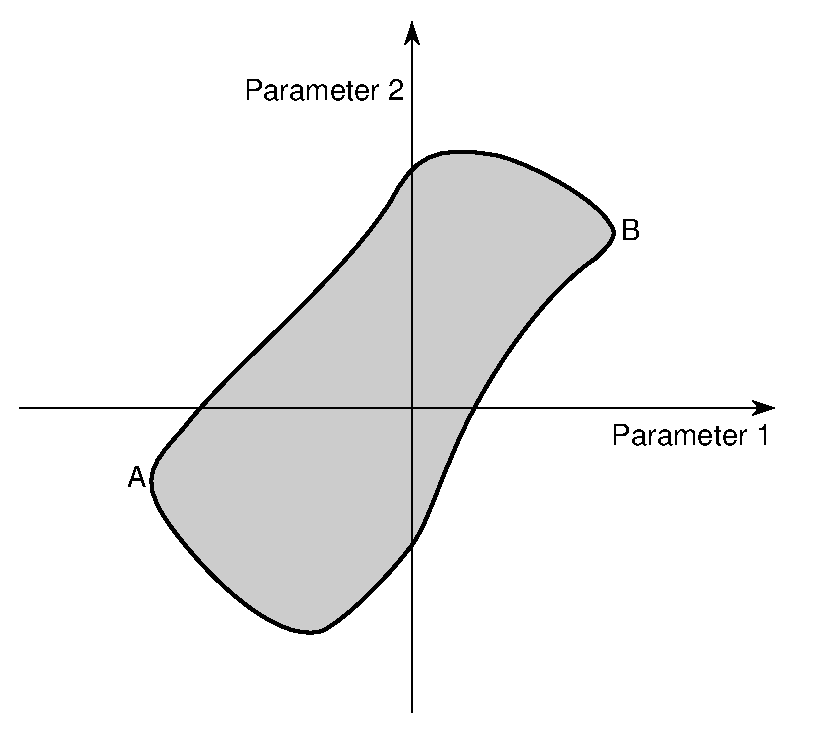
\includegraphics[width=\linewidth]{minosco3.eps}
\end{makeimage}
\caption{Optimal confidence region for parameters 1 and 2}
\label{fig:MINosconf3}
\end{figure}
\begin{rawhtml}<P>\end{rawhtml}
\end{htmlonly}
 
\begin{table}[th]
%begin{latexonly}
\begin{center}
\begin{tabular}{|r<{\quad}*{5}{|>{\quad}r<{\quad}}|} 
\hline
\multicolumn{1}{|r}{\ }
   & \multicolumn{5}{|l|}{\qquad Confidence level 
                              (probability contents desired inside}        \\
\multicolumn{1}{|r}{Number of} 
   & \multicolumn{5}{|l|}{\phantom{\qquad Confidence level (}hypercontour of 
                       $\chi^2 = \chi^2_{\mathrm{min}} + \mbox{\tt UP}$)}  \\
                       \cline{2-6}
\multicolumn{1}{|r|}{Parameters}
          & 50\%   &  70\%  &  90\%  &  95\%  &  99\%  \\
\hline 
1         &  0.46  &  1.07  &  2.70  &  3.84  &  6.63  \\
2         &  1.39  &  2.41  &  4.61  &  5.99  &  9.21  \\
3         &  2.37  &  3.67  &  6.25  &  7.82  & 11.36  \\
4         &  3.36  &  4.88  &  7.78  &  9.49  & 13.28  \\
5         &  4.35  &  6.06  &  9.24  & 11.07  & 15.09  \\
6         &  5.35  &  7.23  & 10.65  & 12.59  & 16.81  \\
7         &  6.35  &  8.38  & 12.02  & 14.07  & 18.49  \\
8         &  7.34  &  9.52  & 13.36  & 15.51  & 20.09  \\
9         &  8.34  & 10.66  & 14.68  & 16.92  & 21.67  \\
10        &  9.34  & 11.78  & 15.99  & 18.31  & 23.21  \\
11        & 10.34  & 12.88  & 17.29  & 19.68  & 24.71  \\
                       \cline{2-6}
& \multicolumn{5}{l|}{\qquad If \protect\Rind{FCN} is $-\log(\mathrm{likelihood})$
                             instead of $\chi^2$, all values of \texttt{UP} }        \\
& \multicolumn{5}{l|}{\qquad should be divided by 2.}                             \\
\hline
\end{tabular}
\end{center}
%end{latexonly}
\begin{htmlonly}
\begin{tabular}{|r|r|r|r|r|r|}
   & \multicolumn{5}{|c|}{Confidence level}\\
\multicolumn{1}{|r}{Nb. parameters}
   & \multicolumn{5}{|c|}{(probability contents desired inside hypercontour
                       $\chi^2 = \chi^2_{\mathrm{min}} + \mathtt{UP}$)}  \\
          & 50\%   &  70\%  &  90\%  &  95\%  &  99\%  \\
1         &  0.46  &  1.07  &  2.70  &  3.84  &  6.63  \\
2         &  1.39  &  2.41  &  4.61  &  5.99  &  9.21  \\
3         &  2.37  &  3.67  &  6.25  &  7.82  & 11.36  \\
4         &  3.36  &  4.88  &  7.78  &  9.49  & 13.28  \\
5         &  4.35  &  6.06  &  9.24  & 11.07  & 15.09  \\
6         &  5.35  &  7.23  & 10.65  & 12.59  & 16.81  \\
7         &  6.35  &  8.38  & 12.02  & 14.07  & 18.49  \\
8         &  7.34  &  9.52  & 13.36  & 15.51  & 20.09  \\
9         &  8.34  & 10.66  & 14.68  & 16.92  & 21.67  \\
10        &  9.34  & 11.78  & 15.99  & 18.31  & 23.21  \\
11        & 10.34  & 12.88  & 17.29  & 19.68  & 24.71  \\
                       \cline{2-6}
& \multicolumn{5}{l|}{For \protect\Rind{FCN} $-\log(\mathrm{likelihood})$
                      instead of $\chi^2$, all values of
                      \texttt{UP} to be divided by 2.}                             
\end{tabular}
\end{htmlonly}
\caption{Table of \texttt{UP} for multi-parameter confidence regions}
\label{tab:MINosconf}
\end{table}

 

%  ==================== Backmaterial ===========================
\begin{thebibliography}{11}

\bibitem{bib-LATEX}
L.~Lamport.
\newblock {\it {\LaTeX} {A Document Preparation System}}.
\newblock Addison-Wesley, 1986.

\bibitem{bib-HBOOK}
R.Brun.
\newblock {\it HBOOK users guide (Version 4.15), {\normalshape Program Library
  Y250}}.
\newblock CERN, 1992.

\bibitem{bib-PAW}
R.Brun, O.Couet, C.Vandoni, and P.Zanarini.
\newblock {\it PAW users guide, {\normalshape Program Library Q121}}.
\newblock CERN, 1991.

\bibitem{bib-MIN81}
F.James.
\newblock {Determining the statistical Significance of experimental Results}.
\newblock Technical Report DD/81/02 and CERN Report 81--03, CERN, 1981.

\bibitem{bib-EADIE}
W.T.Eadie, D.Drijard, F.James, M.Roos, and B.Sadoulet.
\newblock {\it Statistical Methods in Experimental Physics}.
\newblock North-Holland, 1971.

\bibitem{Kowa}
J. Kowalik and M.R. Osborne. 
{\it Methods for unconstrained optimization problems}. 
American Elsevier Publishing Co., Inc., New York, 1968.

\bibitem{Rose}
H.H. Rosenbrock. 
An automatic method for finding the greatest or least value of a function, 
Comput. J.{\bf 3}, 175 (1960).

\bibitem{Hook}
R. Hooke and T.A. Jeeves. 
Direct search solution of numerical an statistical problems.
J. Assoc. Comput. Mach. {\bf 8}, 212 (1961).

\bibitem{Dixo}
L.C.W. Dixon. 
{\it Non-linear optimization}.
English Universities Press, London, 1972.

\bibitem{Neld} 
J.A. Nelder and R. Mead. 
A simplex method for function minimization.
Comput. J. {\bf 7}, 308 (1965).

\bibitem{Stew}
G.W. Stewart. 
A modification of Davidon's method to accept difference approximations 
      of derivatives. 
J. Assoc. Comput. Mach {\bf 14}, 72 (1967).

\bibitem{Flet1} 
R. Fletcher and C.M. Reeves. 
Function minimization by conjugate gradients. 
Comput. J. {\bf 7}, 149 (1964).

\bibitem{Powe1}
M.J.D. Powell. 
An efficient method for finding the minimum of a
        function of several variables without calculating derivatives.
Comput. J. {\bf 7}, 155 (1964).

\bibitem{Land} 
L.D. Landau and E.M. Lifshitz. 
{\it The classical theory of fields}.
Addison-Wesley Publ. Co., Inc., Reading, Mass., 1951.

\bibitem{Flet} 
R. Fletcher and M.J.D. Powell. 
A rapidly converging descent method for minimization. 
Comput. J. {\bf 6}, 163 (1963).

\bibitem{Davi} 
W.C. Davidon. 
Variance algorithm for minimization. 
Comput. J. {\bf 10}, 406 (1968).

\bibitem{Powe2} 
M.J.D. Powell. 
{\it Rank one methods for unconstrained optimization,
        appearing in Integer and Non-linear Programming}. 
J. Adabie, editor. 
North-Holland Publ. Co., Amsterdam, 1970.

\bibitem{Flet2} 
R. Fletcher. 
A new approach to variable metric algorithms.
Comput. J. {\bf 13}, 317 (1970).

\bibitem{Broy} 
C.G. Broyden. 
Quasi-Newton methods and their application to function minimization. 
Math. Comput. {\bf 21}, 368 (1967).

\bibitem{Gelf} 
I.M. Gelfand and f.L. Tsetlin. 
The principle of non-local search in automatic optimization systems. 
Soviet Phys. Dokl. {\bf 6}, 192 (1961).

\bibitem{Gold1} 
A.A. Goldstein and J.F. Price. 
On descent from local minima. 
Math.  Comput . {\bf 25}, 569 (1971).

\bibitem{Flet3} 
R. Fletcher. 
Methods for the solution of optimization problems.
Comput. Phys. Commun. {\bf 3}, 159 (1972).

\bibitem{Powe3} 
M.J.D. Powell. 
A survey of numerical methods for unconstrained optimization. 
SIAM Rev. {\bf 12}, 79 (1970).

\bibitem{Powe4} 
M.J.D. Powell. 
A method for minimizing a sum of squares of non-linear functions 
           without calculating derivatives. 
Comput. J. {\bf 7} 303 (1965).

\bibitem{Gree} 
J. Greenstadt. 
On the relative efficiencies of gradient methods.
Math. Comput. {\bf 21}, 360 (1967) .

\bibitem{Sarg}
R.W.H. Sargent and B.A. Murtaugh. 
Computational experience with quadratically convergent minimization methods. 
Comput. J. {\bf 13} 185 (1970).

\bibitem{Gold2} 
A.A. Goldstein and J.F. Price. 
An effective algorithm for minimization.
Num. Math. {\bf 10}, 184 (1967).

\bibitem{Gill} 
P.E. Gill, W. Murray and M.H. White. 
{\it Practical Optimization}.
Academic Press, 1981.

\end{thebibliography}

%\bibliographystyle{myunsrt} % style for bibliography
%\bibliography{/user/goossens/cnasall/cnasbibl}   % Master BibTeX file for CNAS d

\printindex

\end{document}
